\section{Discrete Forcing Method}
The discrete forcing approach was first introduced in the works of Mohd-Yusof \cite{mohd1997combined} in late nineties. The discrete forcing approach is defining the force in the numerical solution from the known characteristic of the repose. For the case of flow over immersed boundaries, this known characteristic is the flow velocity on the immersed boundary. The general formulation for the discrete forcing method starts with the discretized NS equation

\begin{equation}\label{eq:C3_discreteNSforIndirectForcing}
	\frac{u^{n+1} - u^n}{\Delta t} = RHS^{n+1/2} + f^{n+1/2}
\end{equation}

where $u^{n+1}$ is the velocity at the next time step, $u^n$ is the velocity at the current time step, $\Delta t$ is the time step, and $RHS^{n+1/2}$ contains both the viscous terms and pressure gradient. $f^{n+1/2}$ is the forcing term that needs to be calculated in such a way that yields $u^{n+1} = V$, where $V$ is the known velocity of the immersed boundary. Therefore, the force term is calculated as

\begin{equation}\label{eq:C3_indirectForceing}
	f^{n+1/2} = -RHS^{n+1/2} + \frac{V - u^n}{\Delta t}
\end{equation}

This is valid only if the location of the immersed boundary coincides with the computational nodes. Interpolation from the fluid's computational nodes to the immersed boundary is needed for the cases where the two do not coincide. Depending on how this interpolation is done and where the force terms are calculated, the discrete forcing immersed boundary method is put into two main family based on this.

% -.-.-.-.-.-.-.-.-.-.-.-.-.-.-.-.-.-.-.-.-.-.-.-.-.-.-.-.-.-.-.-.-.-
\subsection{Indirect forcing method}
In the indirect forcing method, the boundary conditions are imposed through a set of forcing terms on nodes near the boundary. These forcing terms are calculated based on the interpolation of a known condition on the immersed boundary from the discretized equations. The forces are applied using delta functions to nodes near the immersed boundary. The interpolation is done as shown in Figure \ref{fig:C3_indiredctForcingMethod}.

\begin{figure}[H]
	\centering
	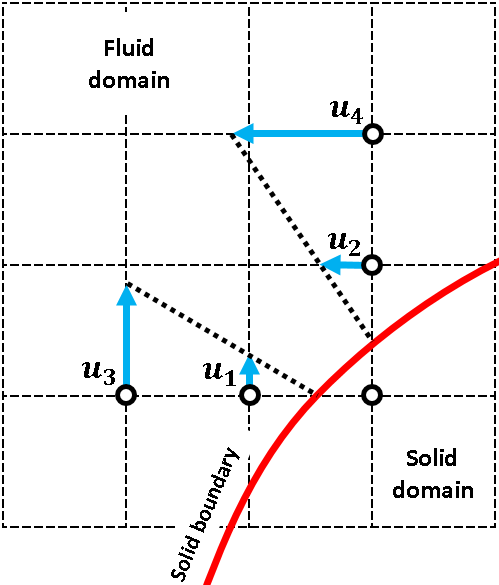
\includegraphics[width=7.00cm]{Chapter_3/figure/indirect_forcing_approach.png}
	\caption{Indirect forcing approach for representing the boundary. The desired velocity values at nodes $1$ and $2$ are interpolated from wall velocity and results from nodes $3$ and $4$.}
	\label{fig:C3_indiredctForcingMethod}
\end{figure}

The force terms are applied on nodes $1$ and $2$ based on the known zero velocity on wall, and a calculated velocity at nodes $3$ and $4$. Linear interpolation is used to calculate the required velocity at nodes $1$ and $2$ so that it results in zero velocity on the immersed boundary. These known velocities are then used in Equation \ref{eq:C3_indirectForceing} to calculate the forcing values. This forcing value is then used in Equation \ref{eq:C3_discreteNSforIndirectForcing} to calculate the velocity field at the next time step.

To investigate the indirect forcing approach, we apply this methodology to the demonstration problem. The investigated three different cases: effect of wall location, effect of node number, and effect of wall velocity. For the first case we selected the wall velocity as $1 m/s$ with $41$ nodes to discretize the domain. The time step of this simulation is selected as $10^{-3}$. The governing equations are discretized using the Euler method in time and second order finite difference method in space as shown in the following equation.

\begin{equation}
	\frac{u(i, n+1) - u(i, n)}{\Delta t} = \frac{u(i - 1, n) - 2u(i, n) + u(i + 1, n)}{(\Delta x)^2} + f(i, n)
\end{equation}

where $u(i, n)$ is the velocity of fluid at location $i$ and time $n$, $\Delta x$ is the nodal distances in sapce, $\Delta t$ is the nodal distance in time, and $f(i,n)$ is the value of forcing function at location $i$ in time $n$. The forcing function is calculated using the linear interpolation based on zero slip condition on the wall. The results for different location of the fixed wall is shown in Figure \ref{fig:C3_indirectForcing_wallLocation} and Table \ref{fig:C3_indirectForcing_wallLocationRSME}. The wall location is selected as $0.178$, $0.351$, $0.612$, $0.842$. As shown here, the wall location with respect to computational nodes does not affect the solution accuracy.

\begin{figure}[H]
	\centering
	\subfigure[$x_{wall} = 0.178$]
	{
	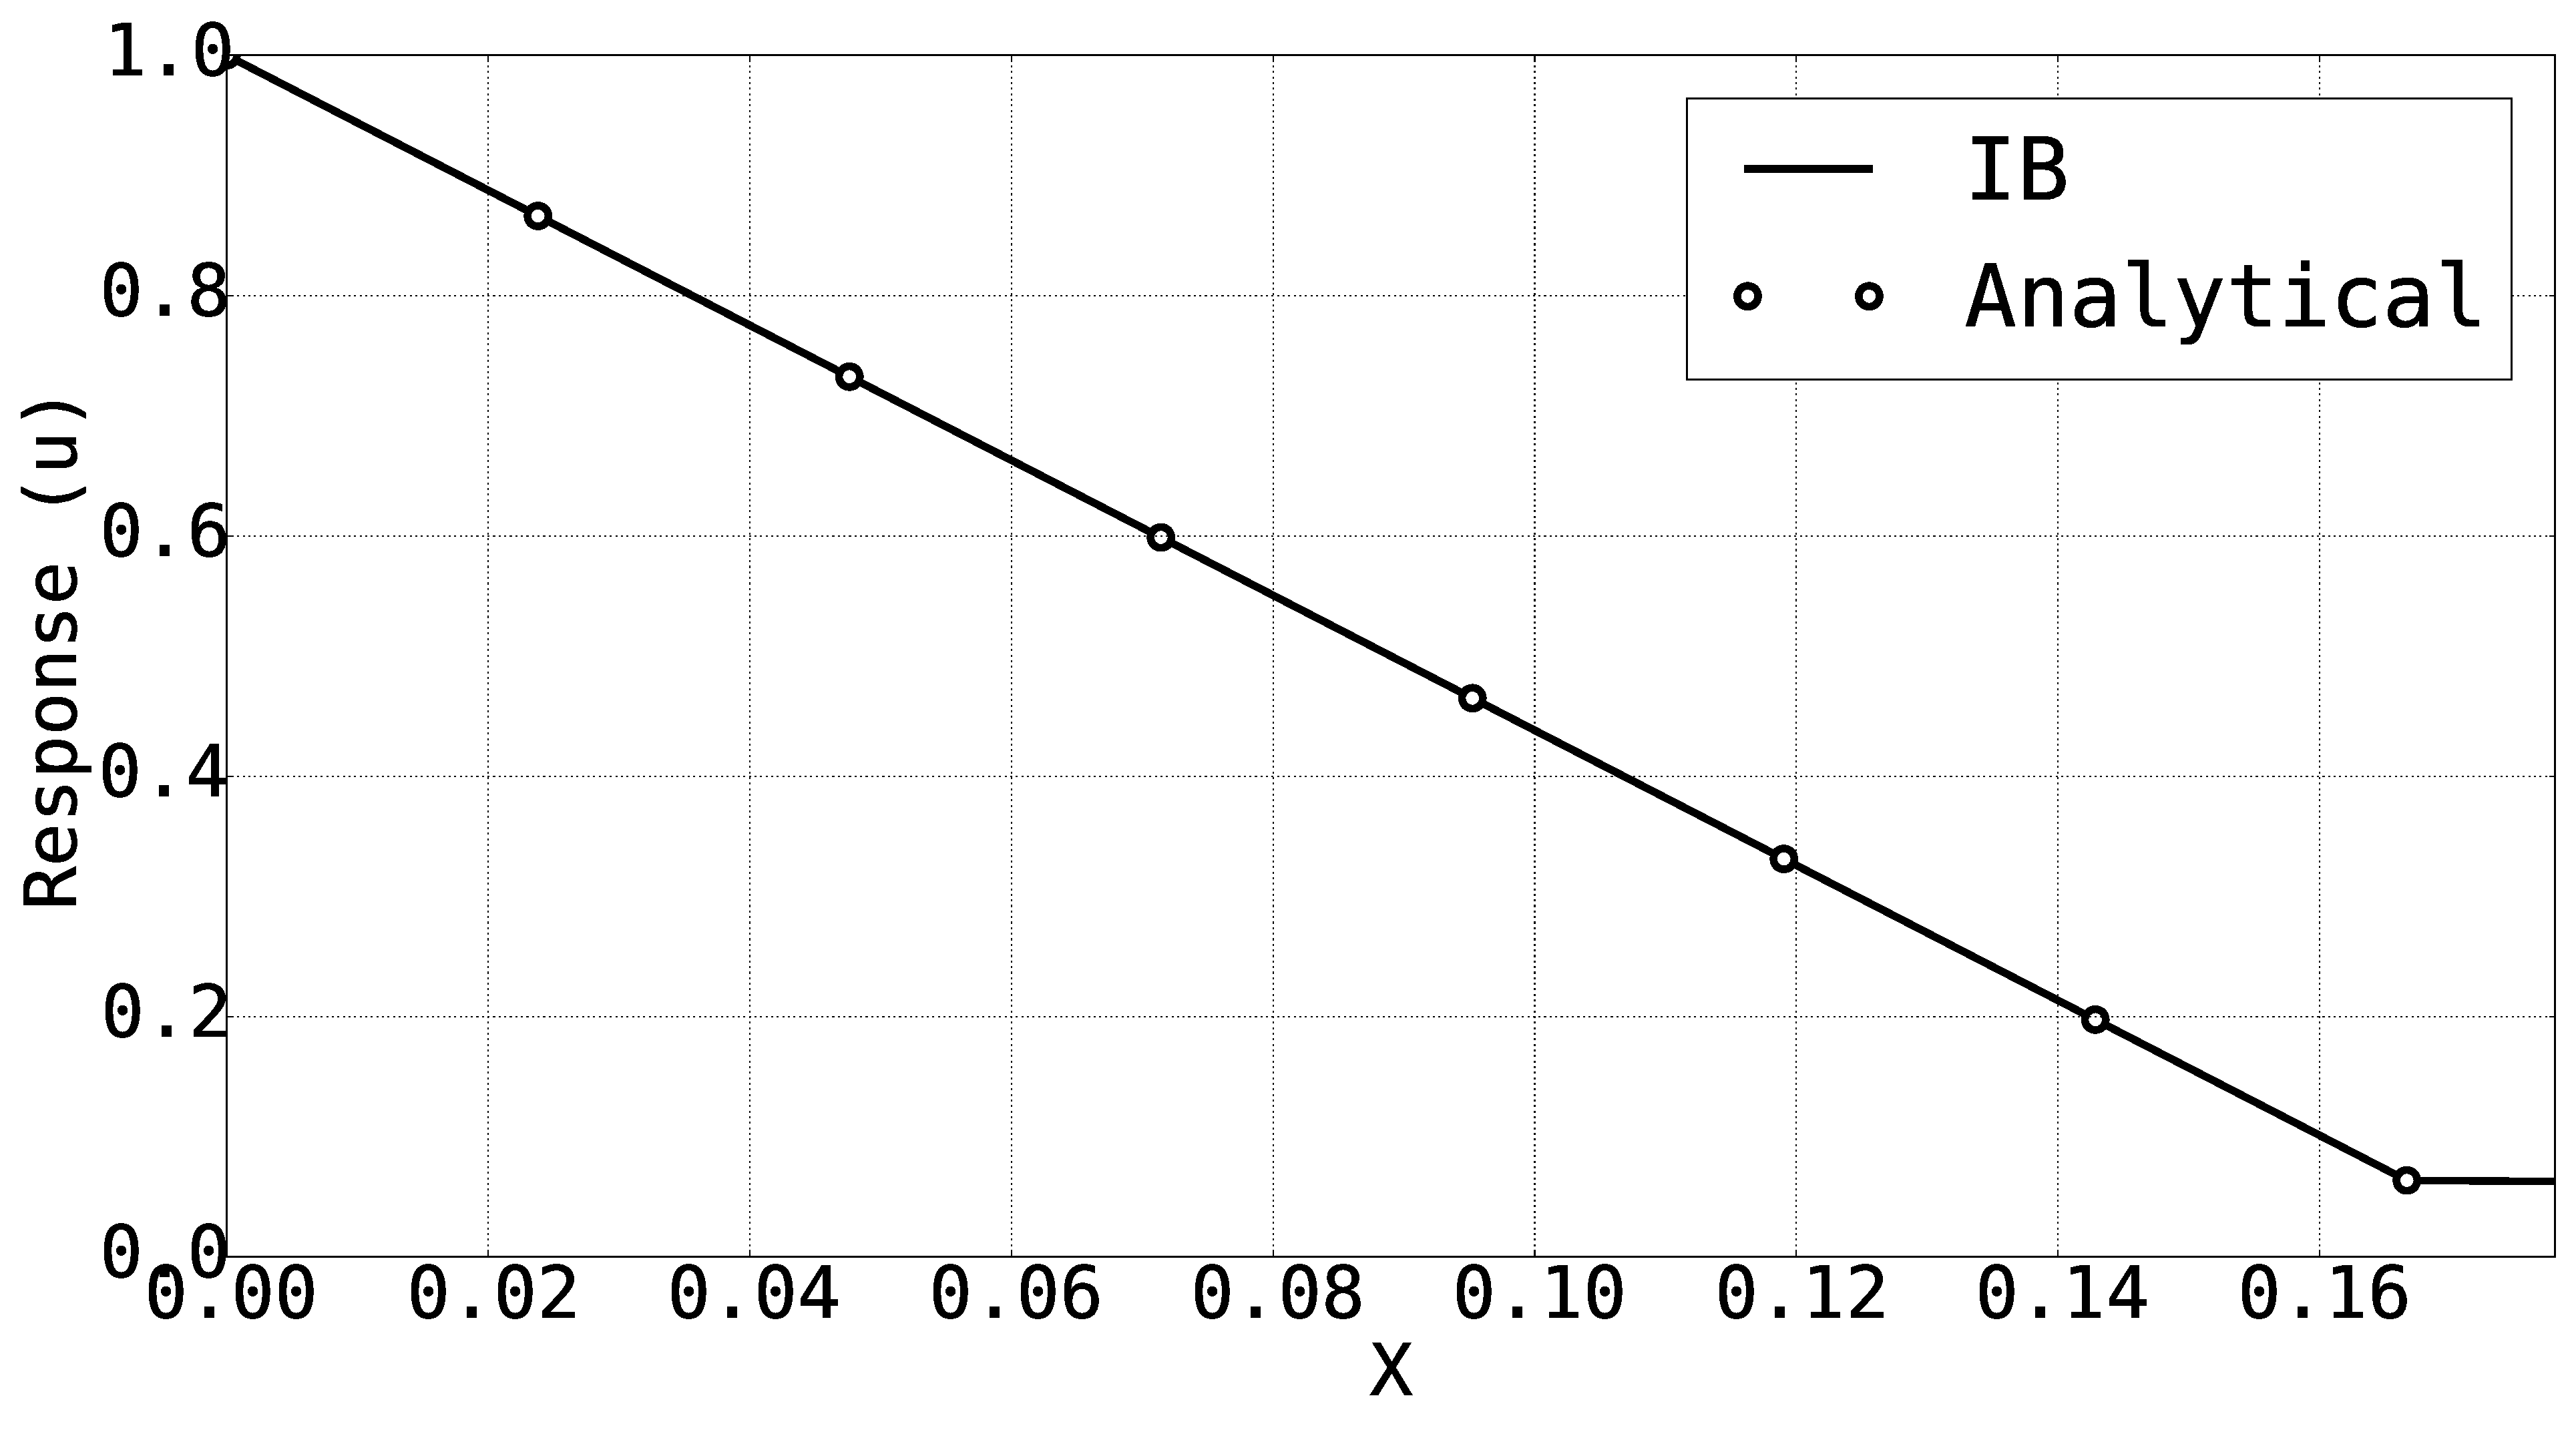
\includegraphics[width=7.0cm]{Chapter_3/figure/indirectForcing_wallLocation_178.eps}
	}
	\quad
	\subfigure[$x_{wall} = 0.351$]
	{
	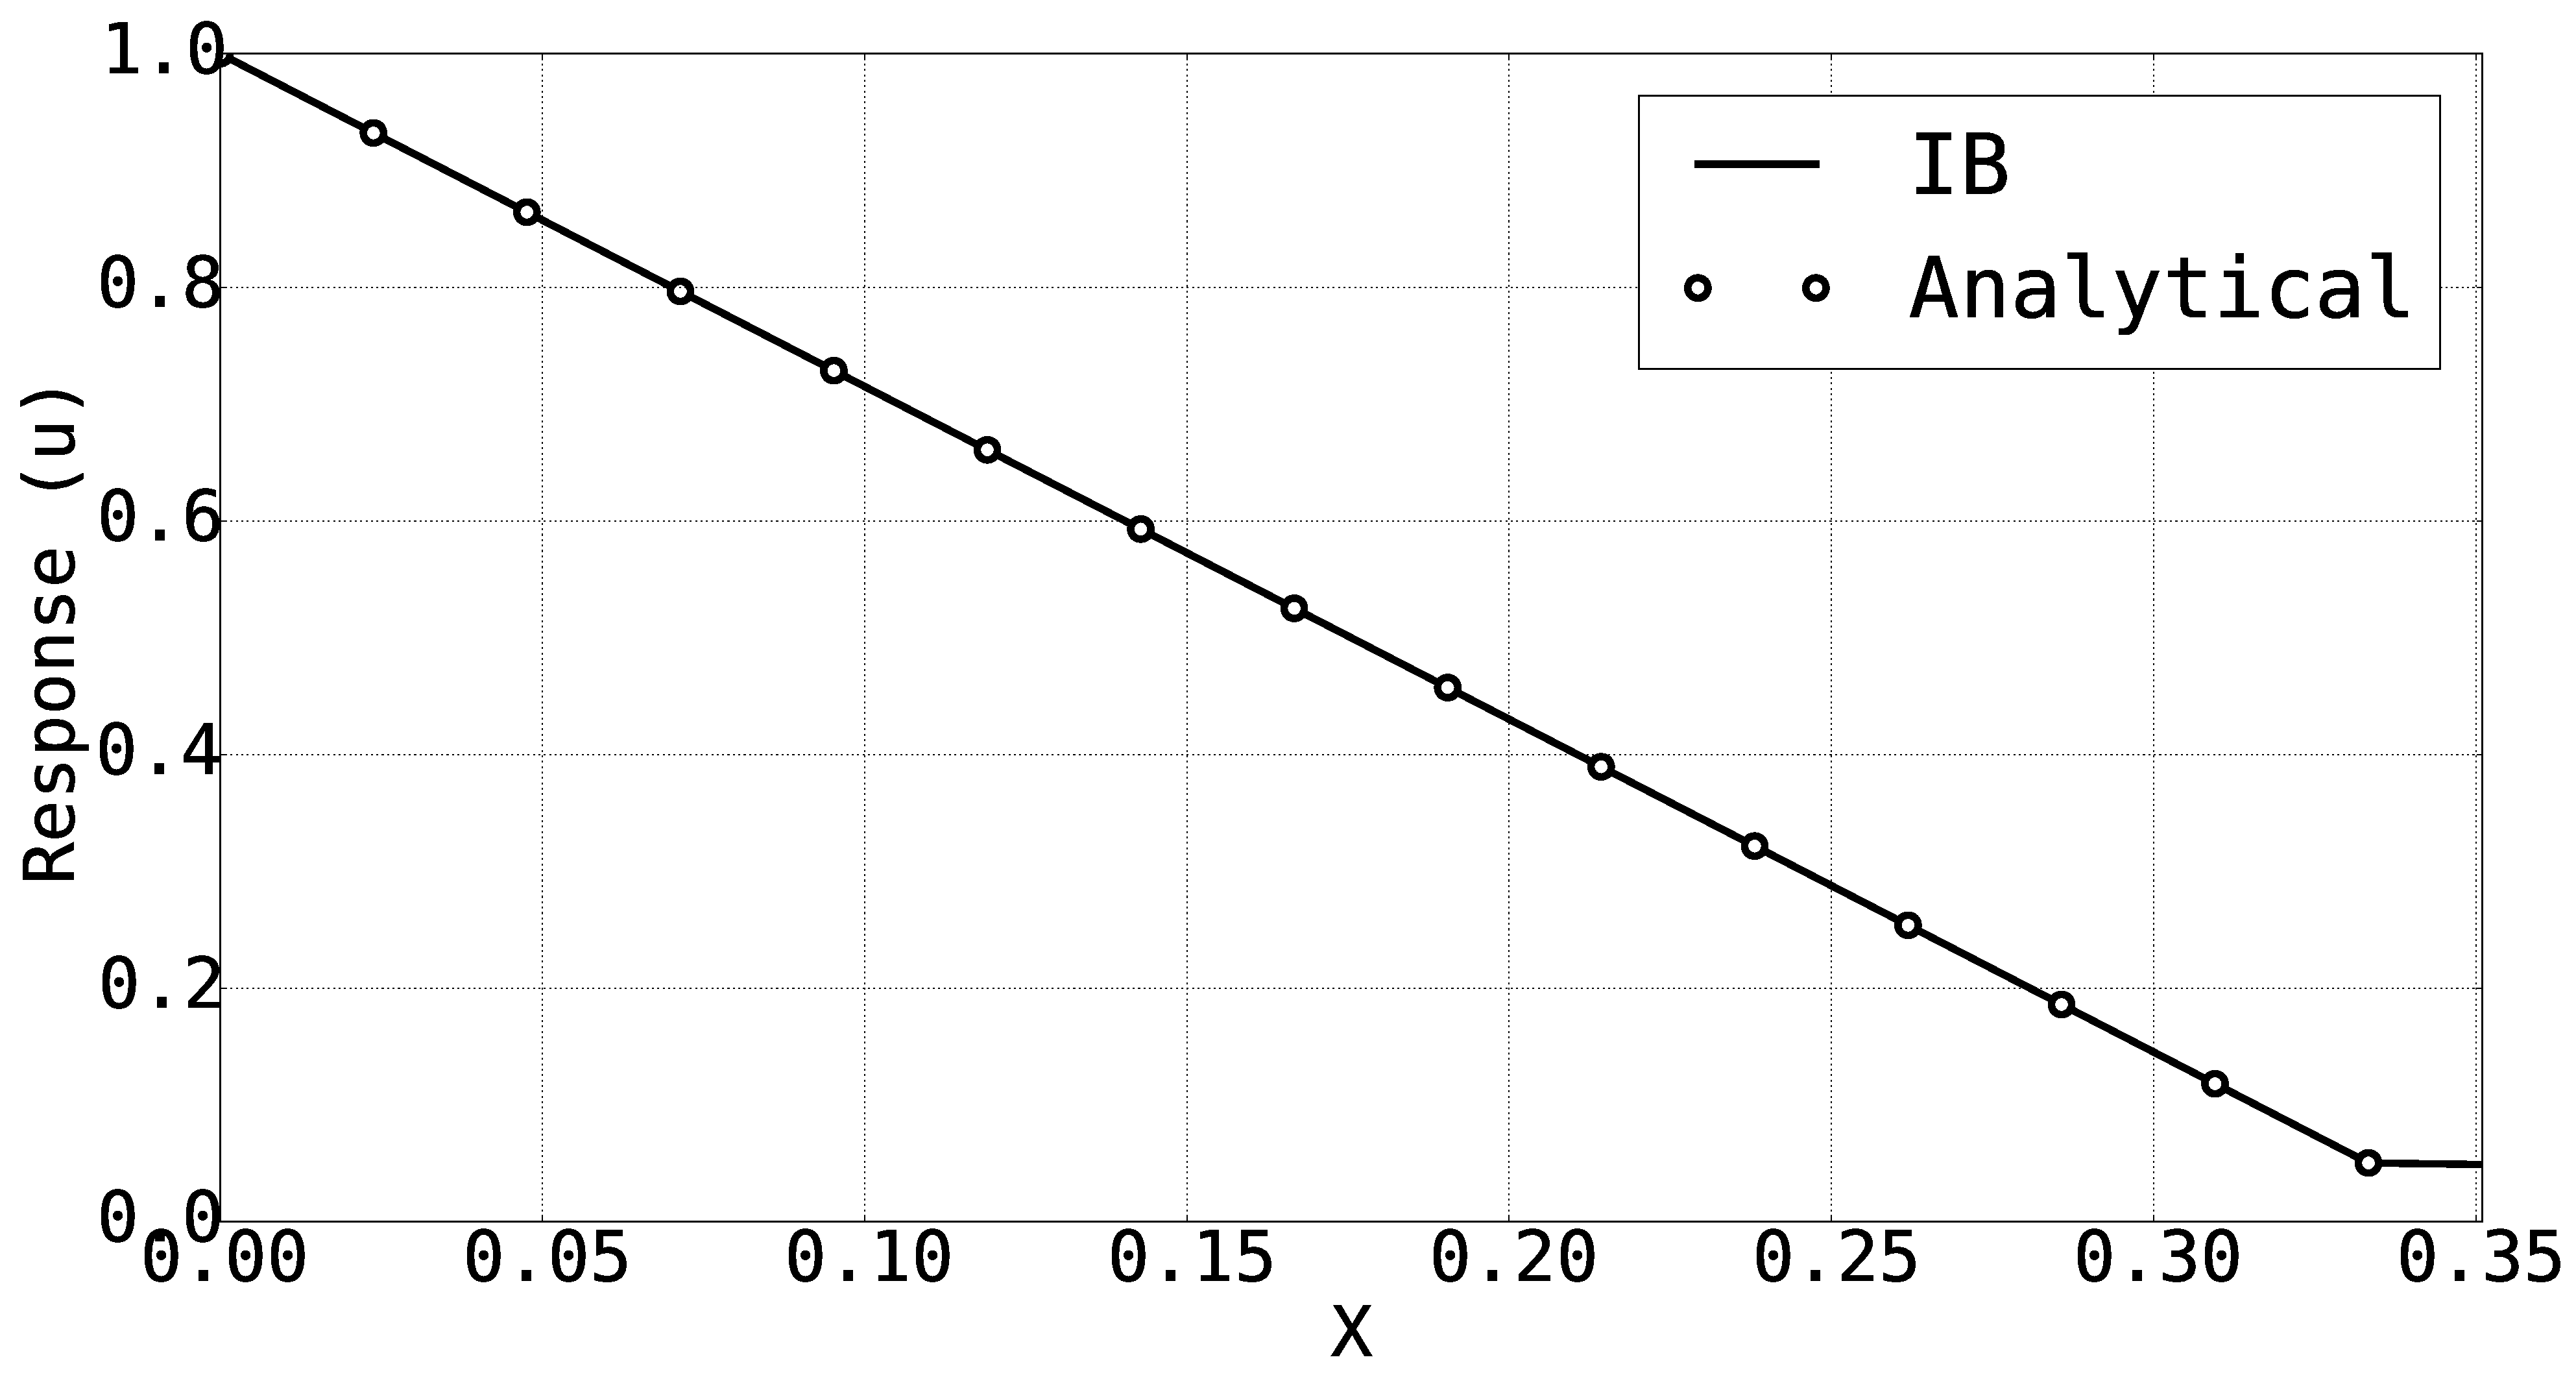
\includegraphics[width=7.0cm]{Chapter_3/figure/indirectForcing_wallLocation_351.eps}
	}
	\\
	\subfigure[$x_{wall} = 0.612$]
	{
	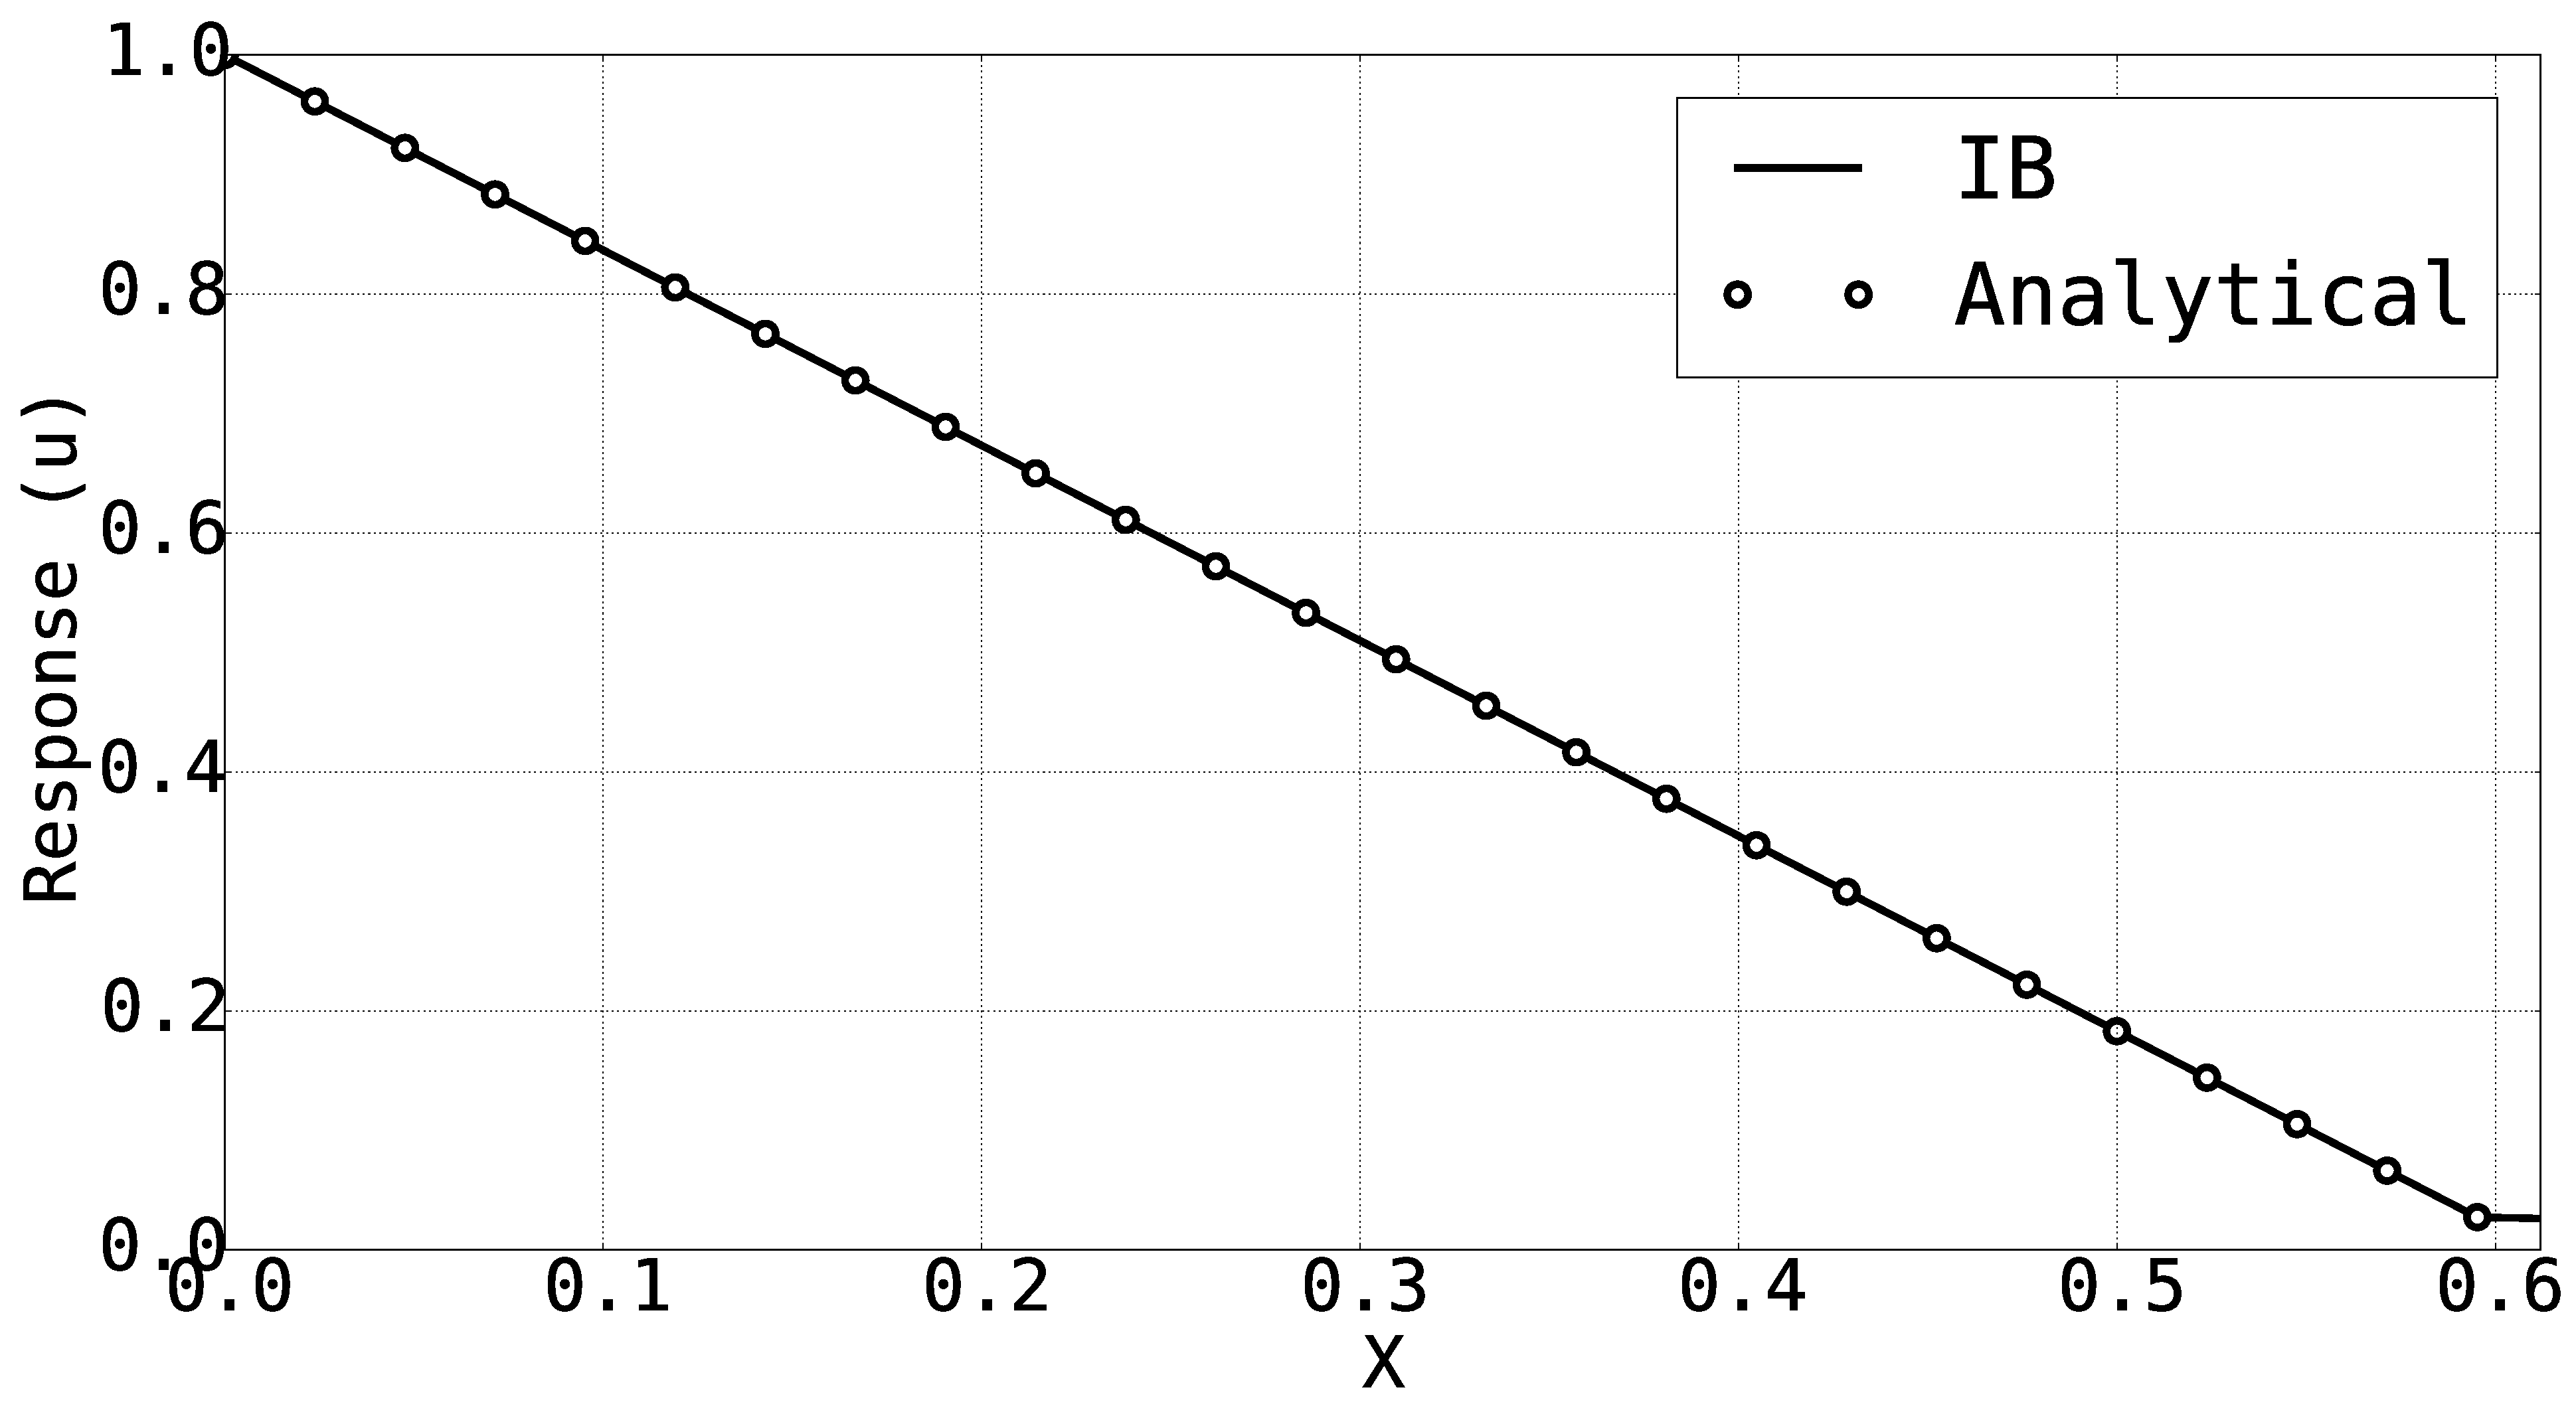
\includegraphics[width=7.0cm]{Chapter_3/figure/indirectForcing_wallLocation_612.eps}
	}
	\quad
	\subfigure[$x_{wall} = 0.842$]
	{
	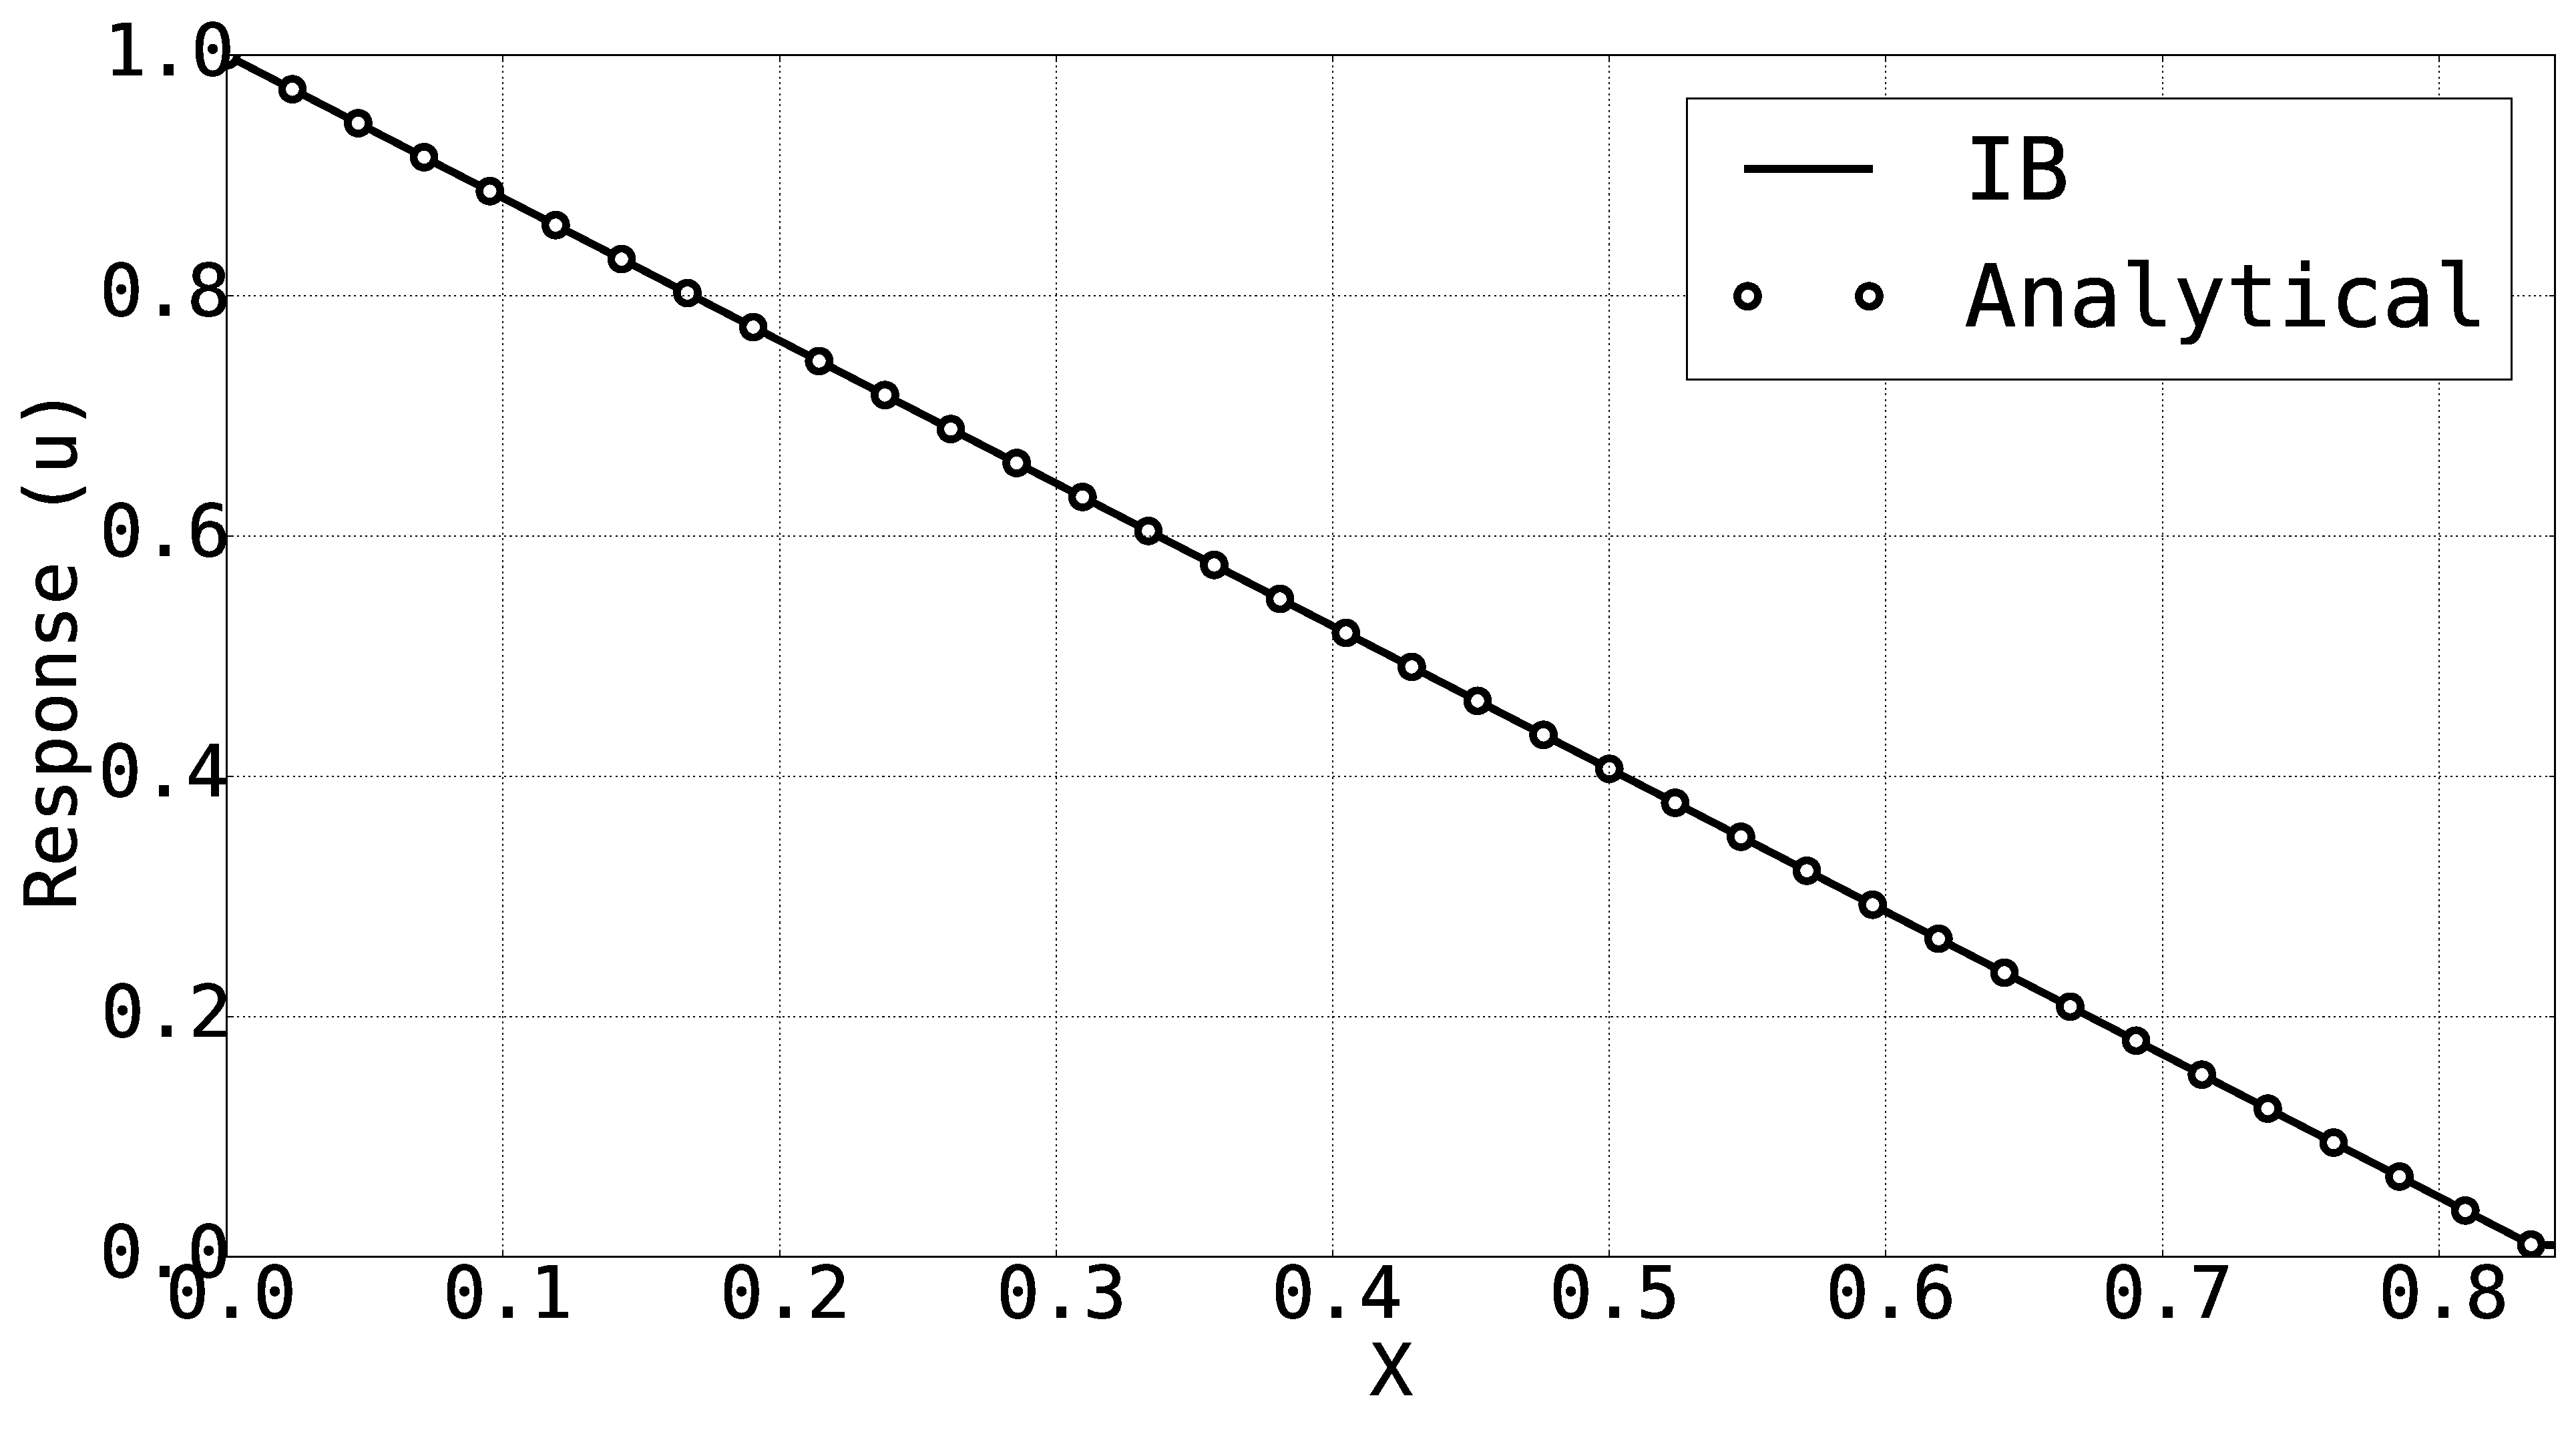
\includegraphics[width=7.0cm]{Chapter_3/figure/indirectForcing_wallLocation_842.eps}
	}
	\caption{Comparison between IB and analytical results for different wall locations.}
	\label{fig:C3_indirectForcing_wallLocation}
\end{figure}

\begin{table}[H]
\centering
\begin{tabular}{c | c}
	 Wall location & RMSE value \\ \hline \hline
	 0.178 & $1.61 \times 10^{-15}$ \\ \hline
	 0.351 & $2.29 \times 10^{-15}$ \\ \hline
	 0.612 & $1.72 \times 10^{-15}$ \\ \hline
	 0.842 & $3.81 \times 10^{-15}$
\end{tabular}
\caption{RMSE value for different wall locations.}
\label{table:C3_indirectForcing_wallLocationRSME}
\end{table}

For the second case, we looked at the effect of node number on the accuracy of the simulation using indirect forcing method. For this case, the wall velocity is fixed at $1 m/s$ and the stationary wall is located at $0.5741$. The number of nodes is chosen as $11$, $41$, $81$, and $161$. As can be seen in Figure \ref{fig:C3_indirectForcing_nodeNumber} and Table \ref{fig:C3_indirectForcing_nodeNumberRSME}, the number of nodes does not affect the accuracy of indirect forcing approach.

\begin{figure}[H]
	\centering
	\subfigure[$x_{wall} = 0.178$]
	{
	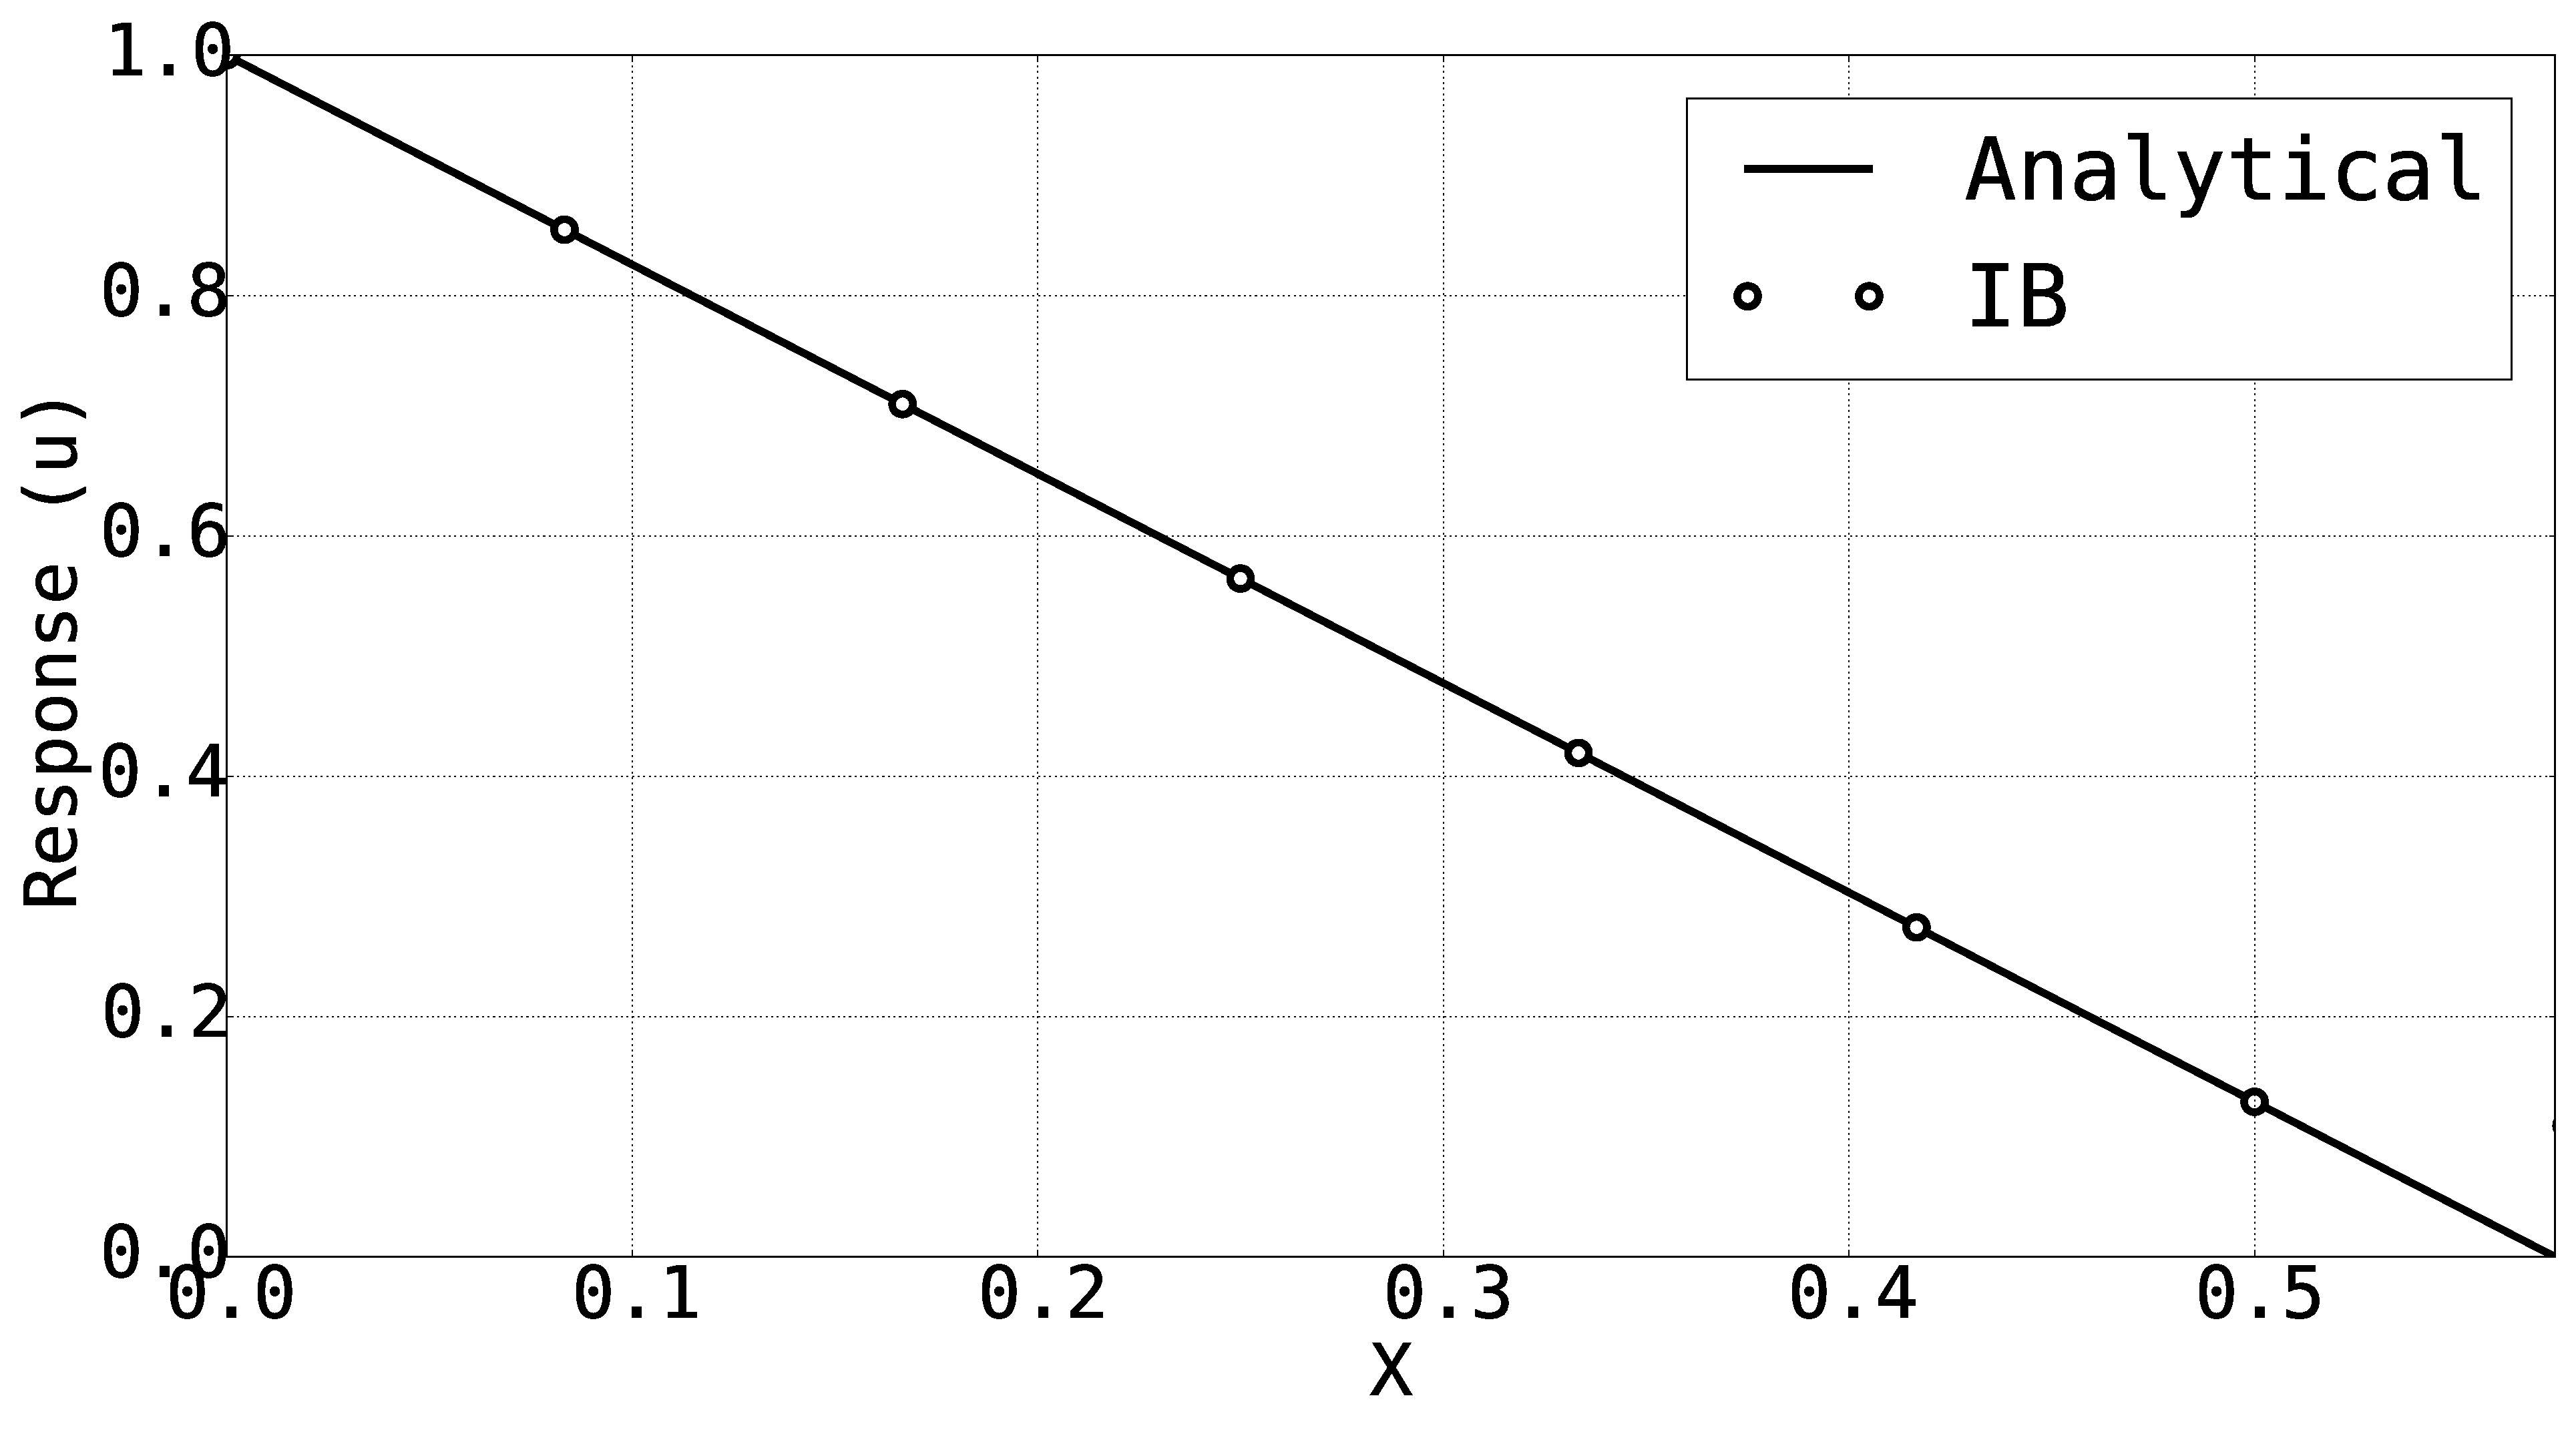
\includegraphics[width=7.0cm]{Chapter_3/figure/indirectForcing_nodeNumber_11.eps}
	}
	\quad
	\subfigure[$x_{wall} = 0.351$]
	{
	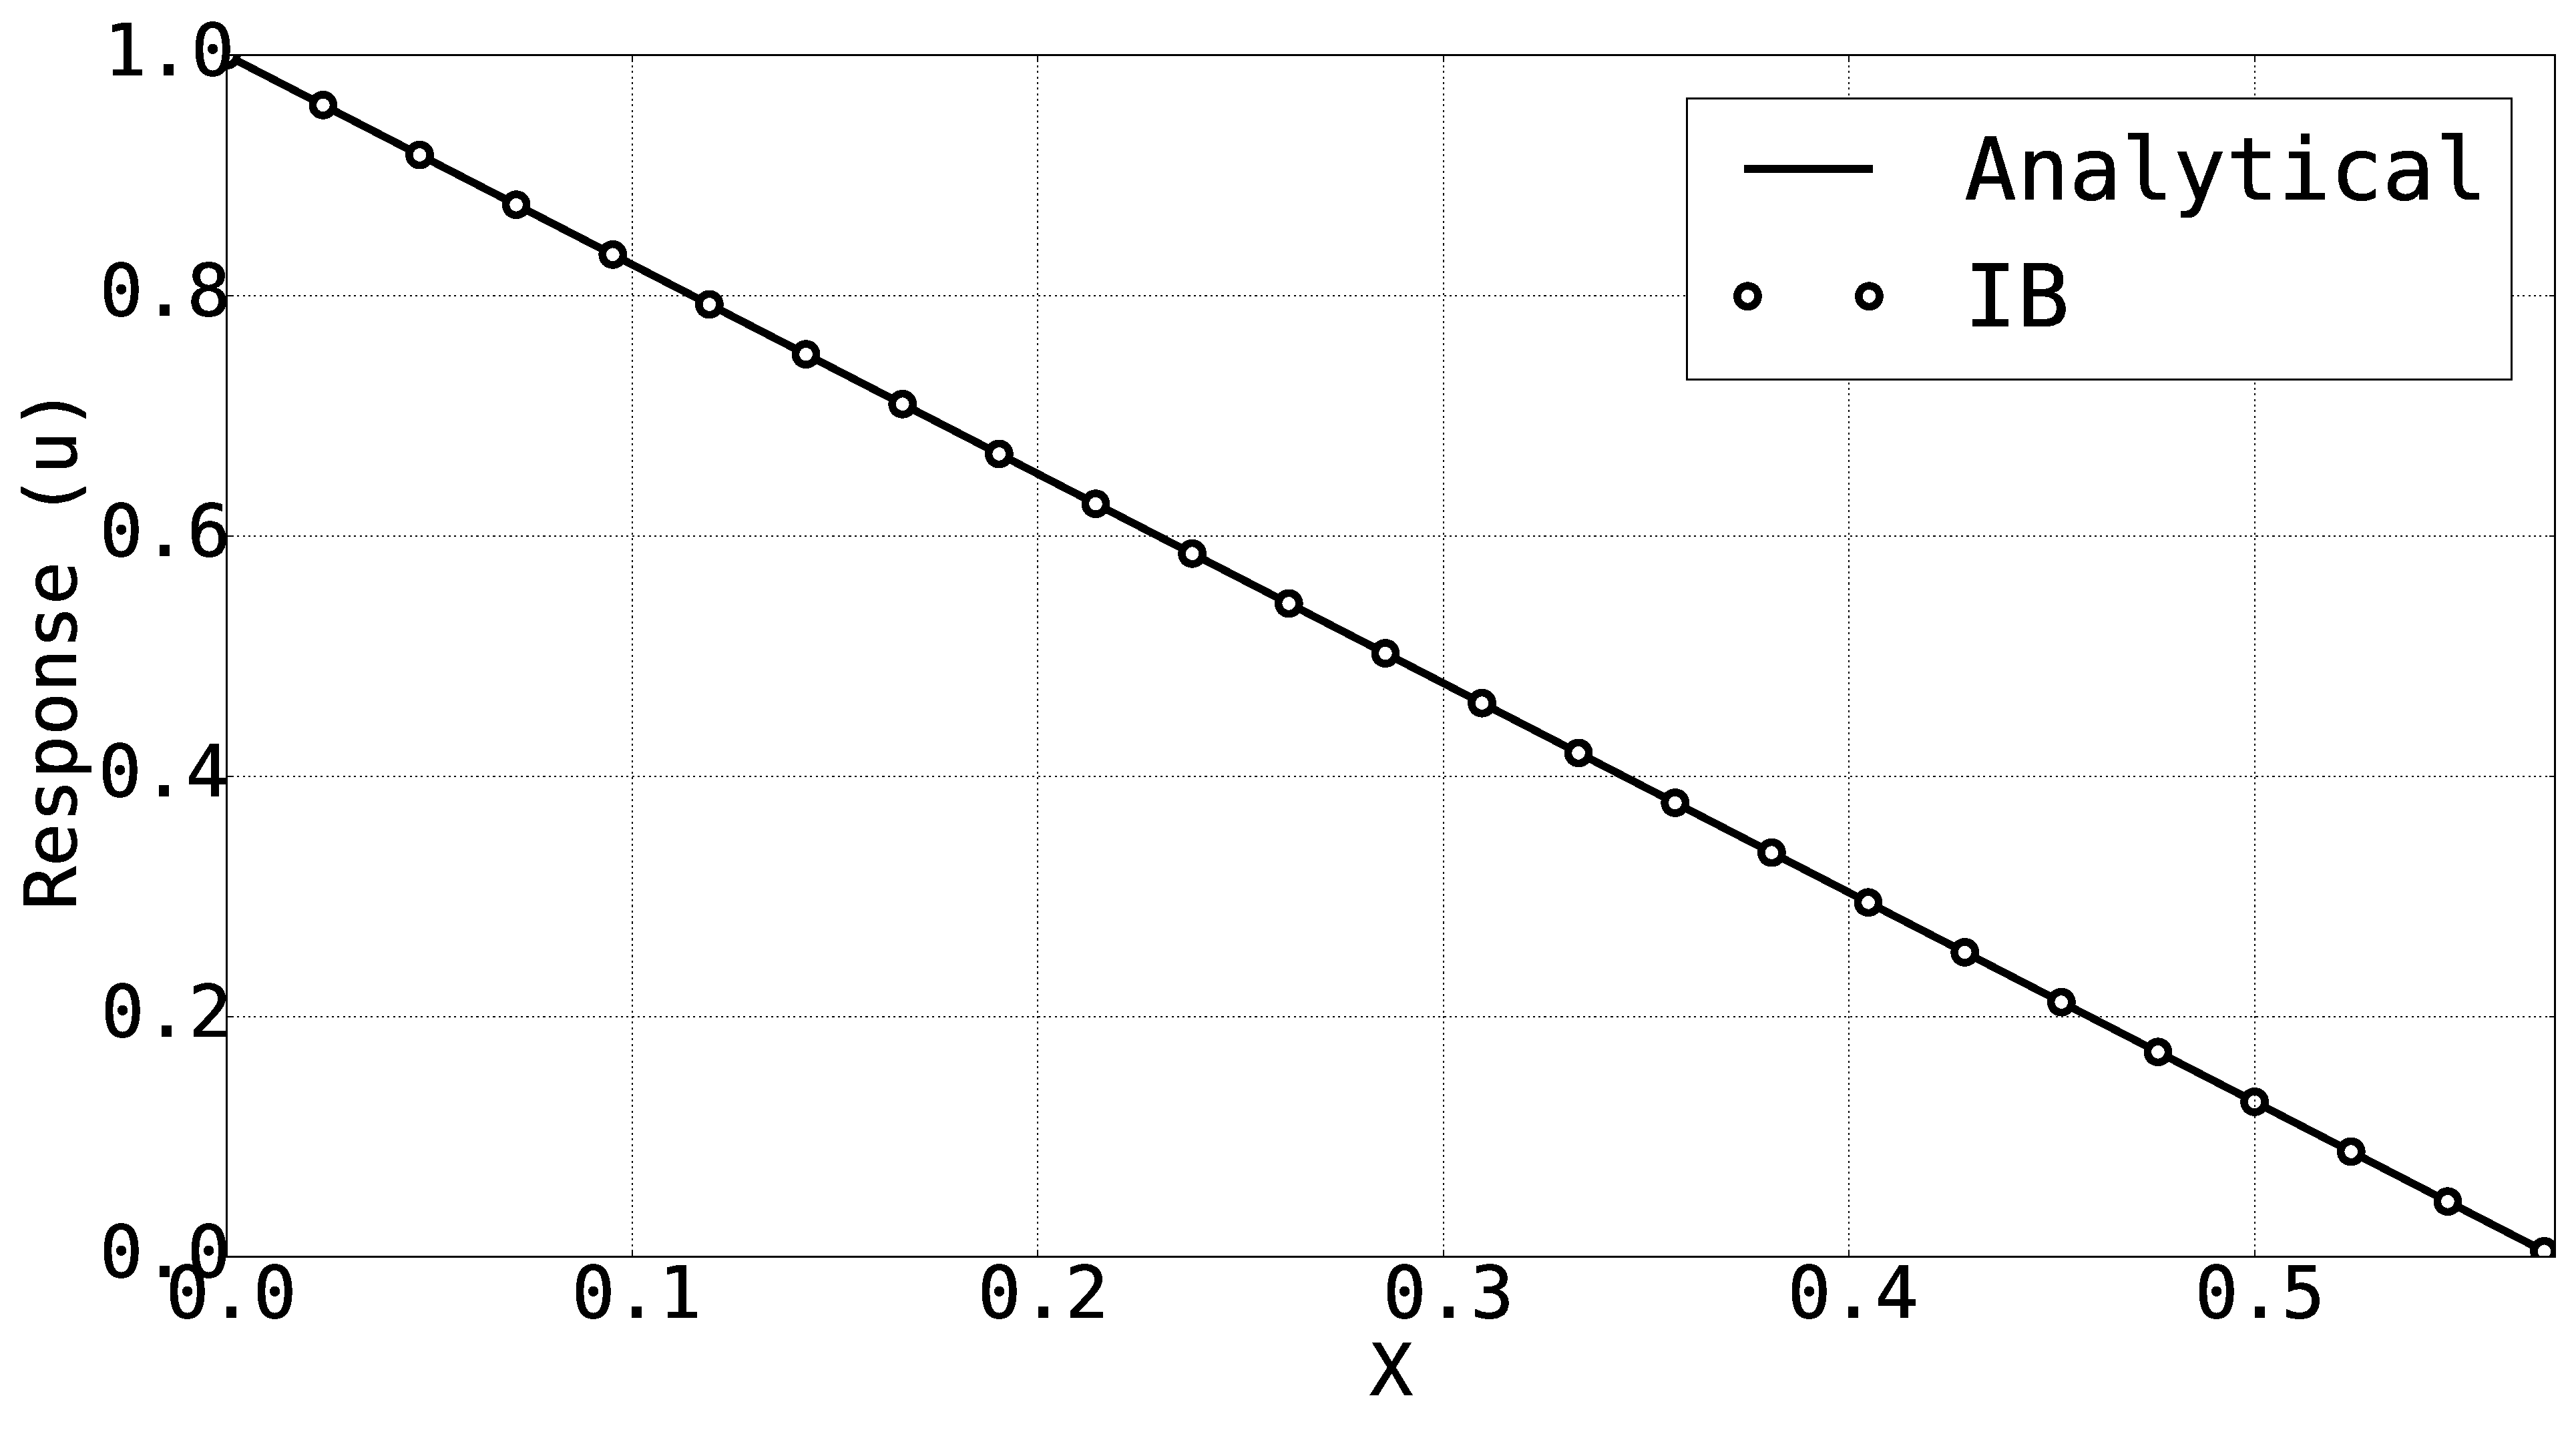
\includegraphics[width=7.0cm]{Chapter_3/figure/indirectForcing_nodeNumber_41.eps}
	}
	\\
	\subfigure[$x_{wall} = 0.612$]
	{
	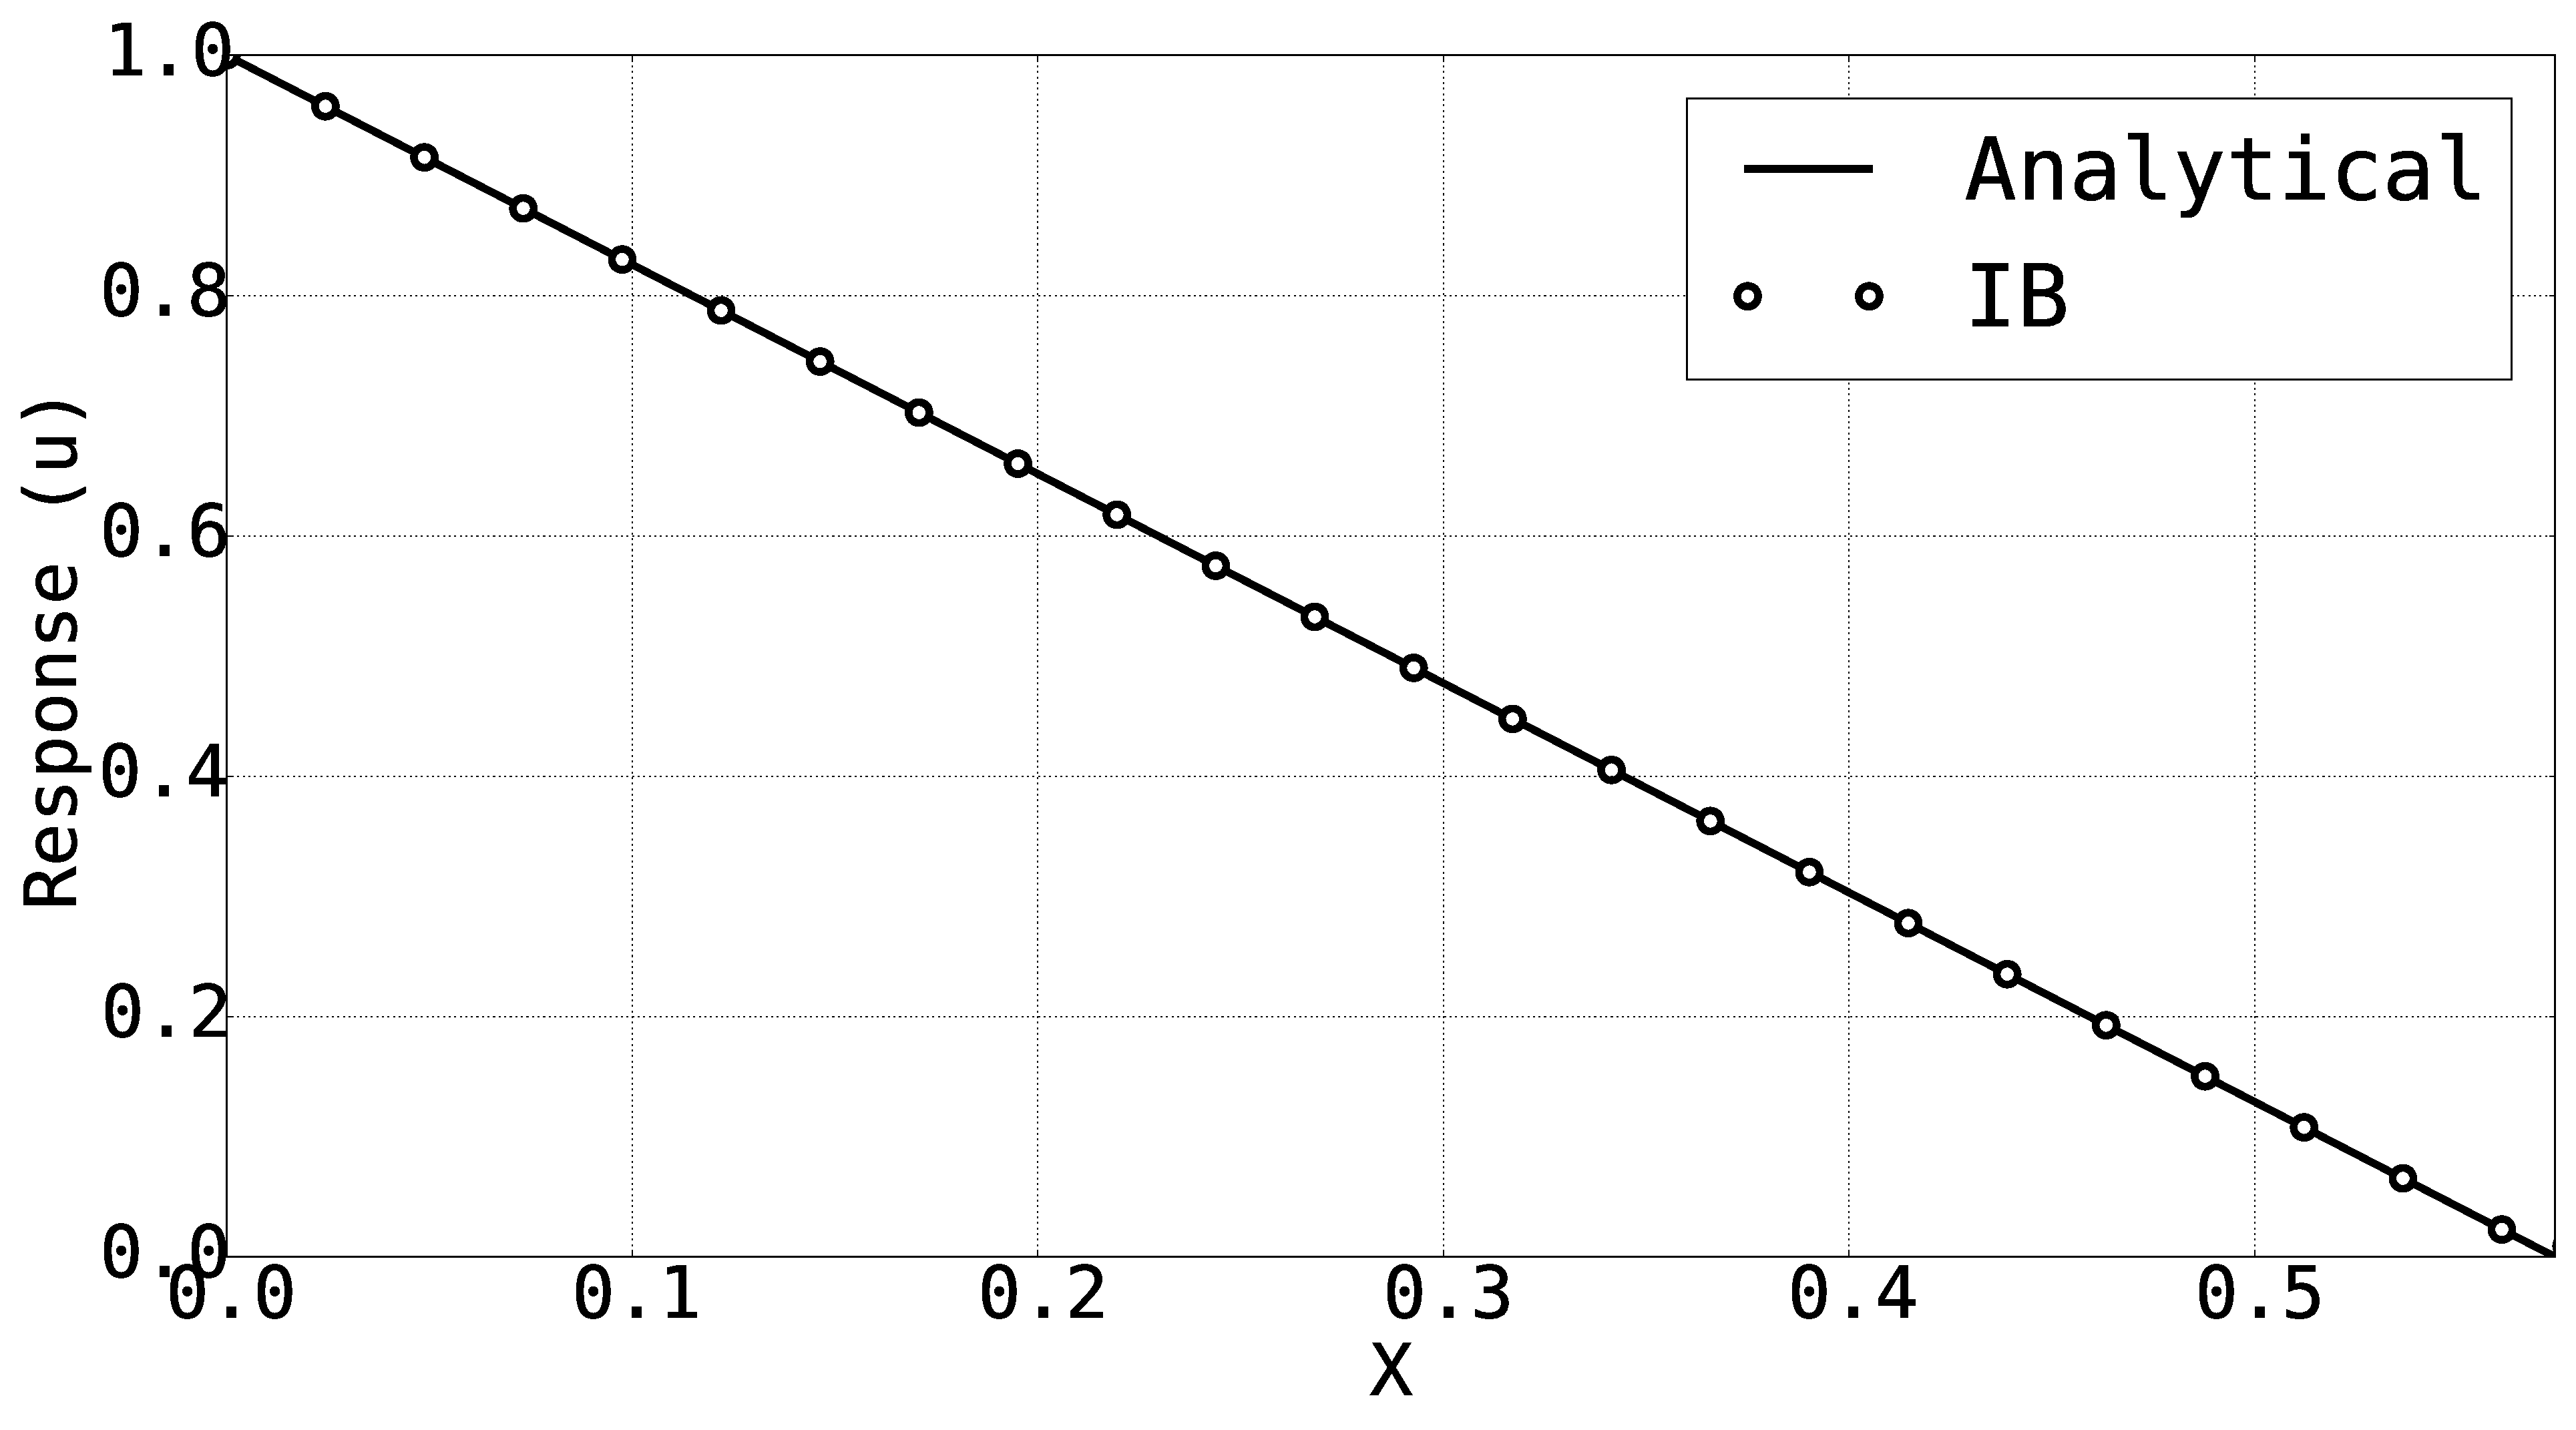
\includegraphics[width=7.0cm]{Chapter_3/figure/indirectForcing_nodeNumber_81.eps}
	}
	\quad
	\subfigure[$x_{wall} = 0.842$]
	{
	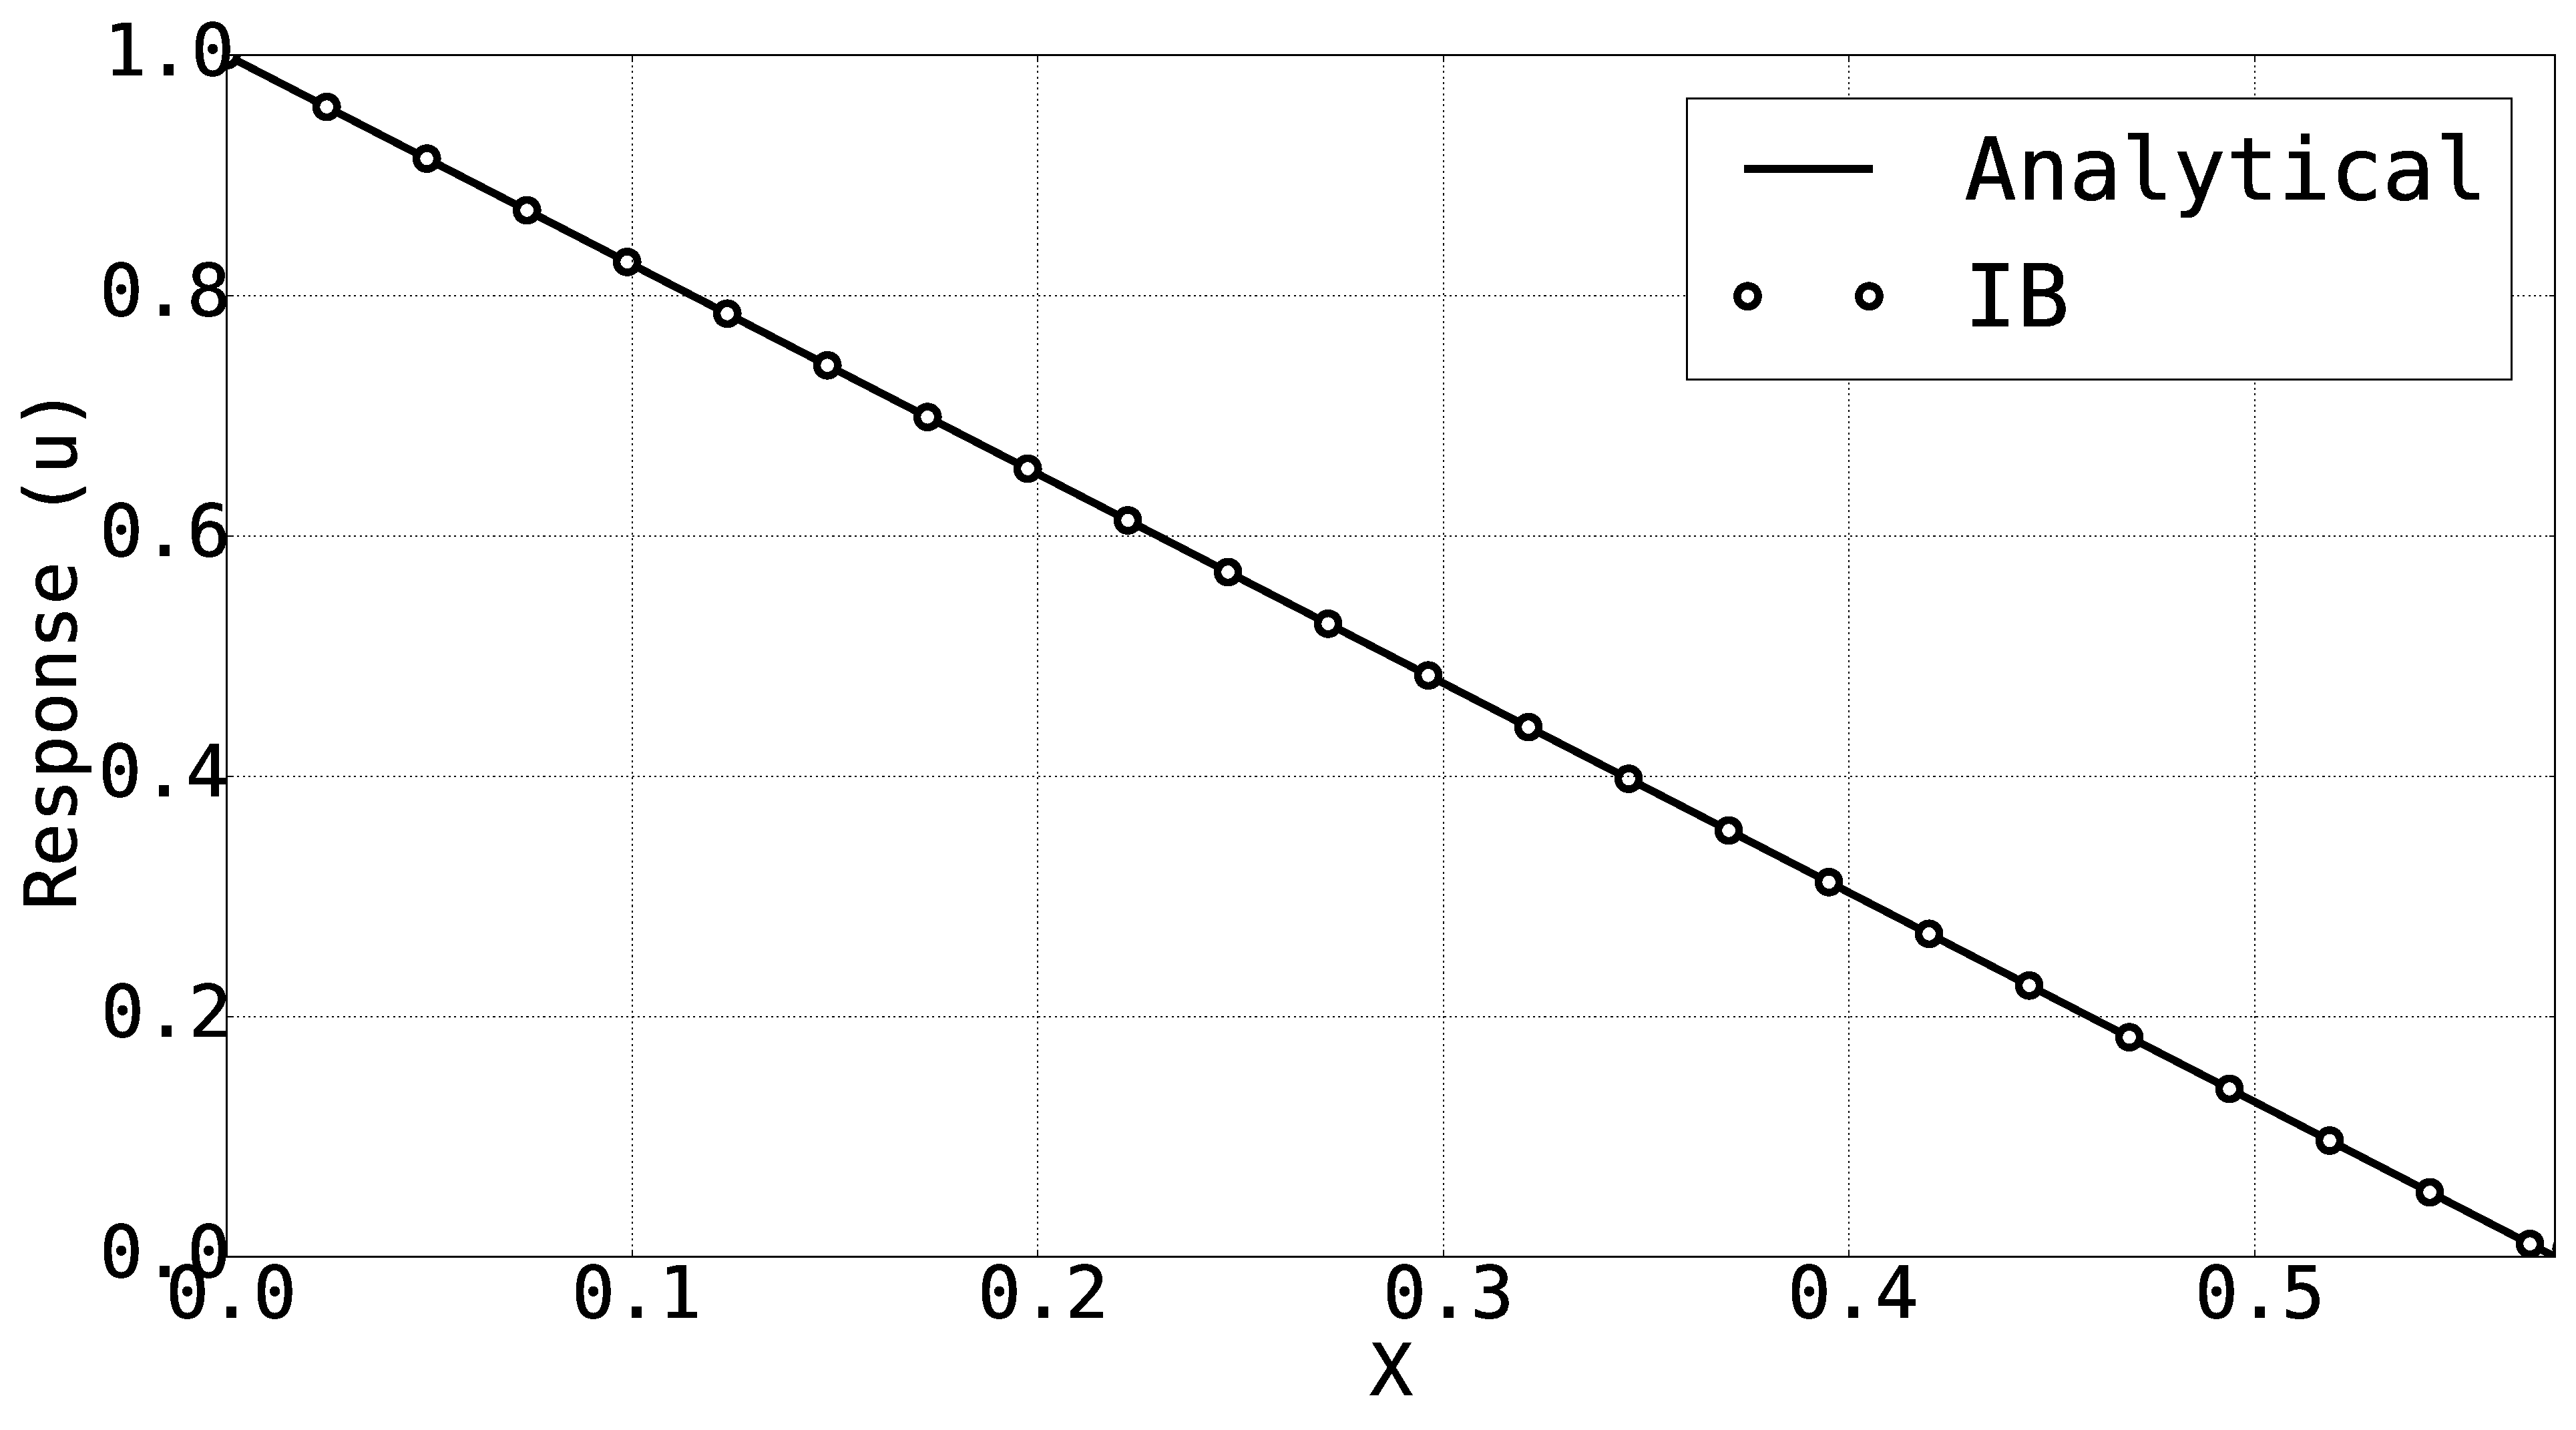
\includegraphics[width=7.0cm]{Chapter_3/figure/indirectForcing_nodeNumber_161.eps}
	}
	\caption{Comparison between IB and analytical results for different node numbers.}
	\label{fig:C3_indirectForcing_nodeNumber}
\end{figure}

\begin{table}[H]
\centering
\begin{tabular}{c | c}
	 Wall location & RMSE value \\ \hline \hline
	 11 & $1.20 \times 10^{-15}$ \\ \hline
	 41 & $1.50 \times 10^{-15}$ \\ \hline
	 81 & $5.64 \times 10^{-15}$ \\ \hline
	 161 & $3.76 \times 10^{-15}$
\end{tabular}
\caption{RMSE value for different node numbers.}
\label{table:C3_indirectForcing_nodeNumberRSME}
\end{table}

For the final case, we looked at the effect of wall velocity on the accuracy of the simulation accuracy. For this case, the node number is fixed at $41$ and the stationary wall is located at $0.5741$. The wall velocity is chosen as $10$, $100$, $1000$, and $10000$. As can be seen in Figure \ref{fig:C3_indirectForcing_wallVelocity} and Table \ref{fig:C3_indirectForcing_wallVelocityRSME}, the wall velocity does not affect the accuracy of indirect forcing approach.

\begin{figure}[H]
	\centering
	\subfigure[$x_{wall} = 0.178$]
	{
	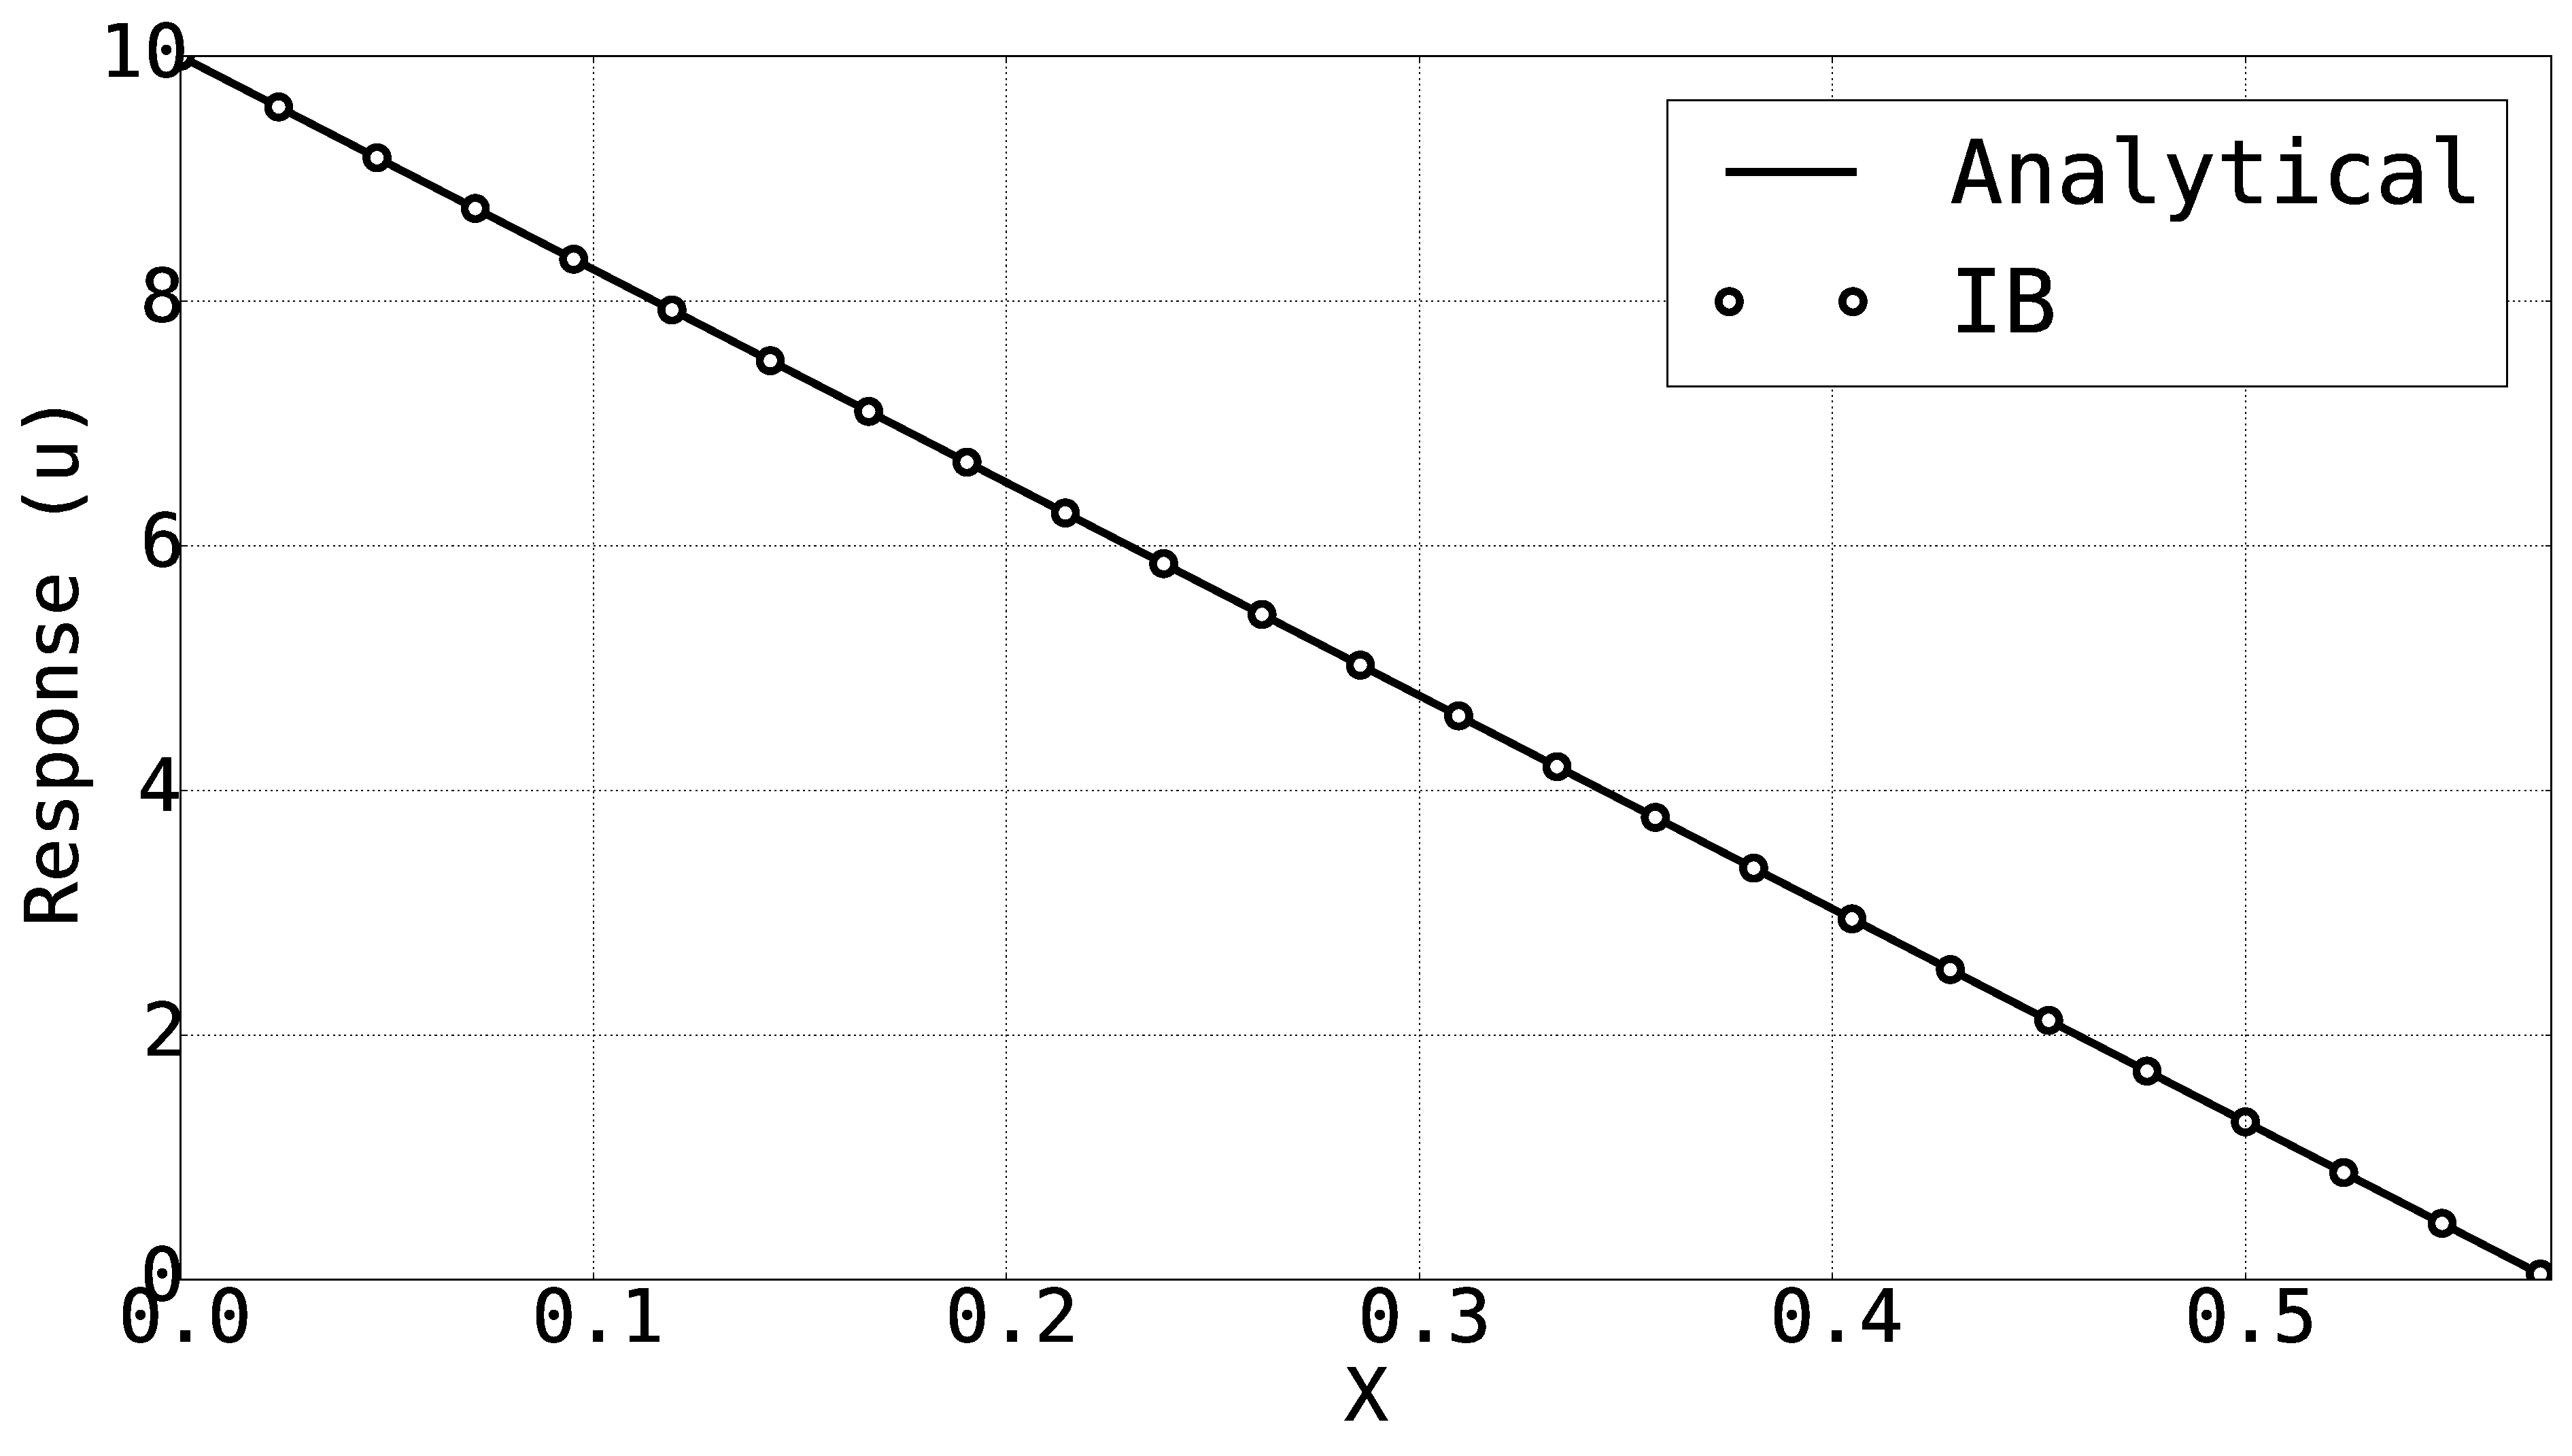
\includegraphics[width=7.0cm]{Chapter_3/figure/indirectForcing_wallVelocity_10.eps}
	}
	\quad
	\subfigure[$x_{wall} = 0.351$]
	{
	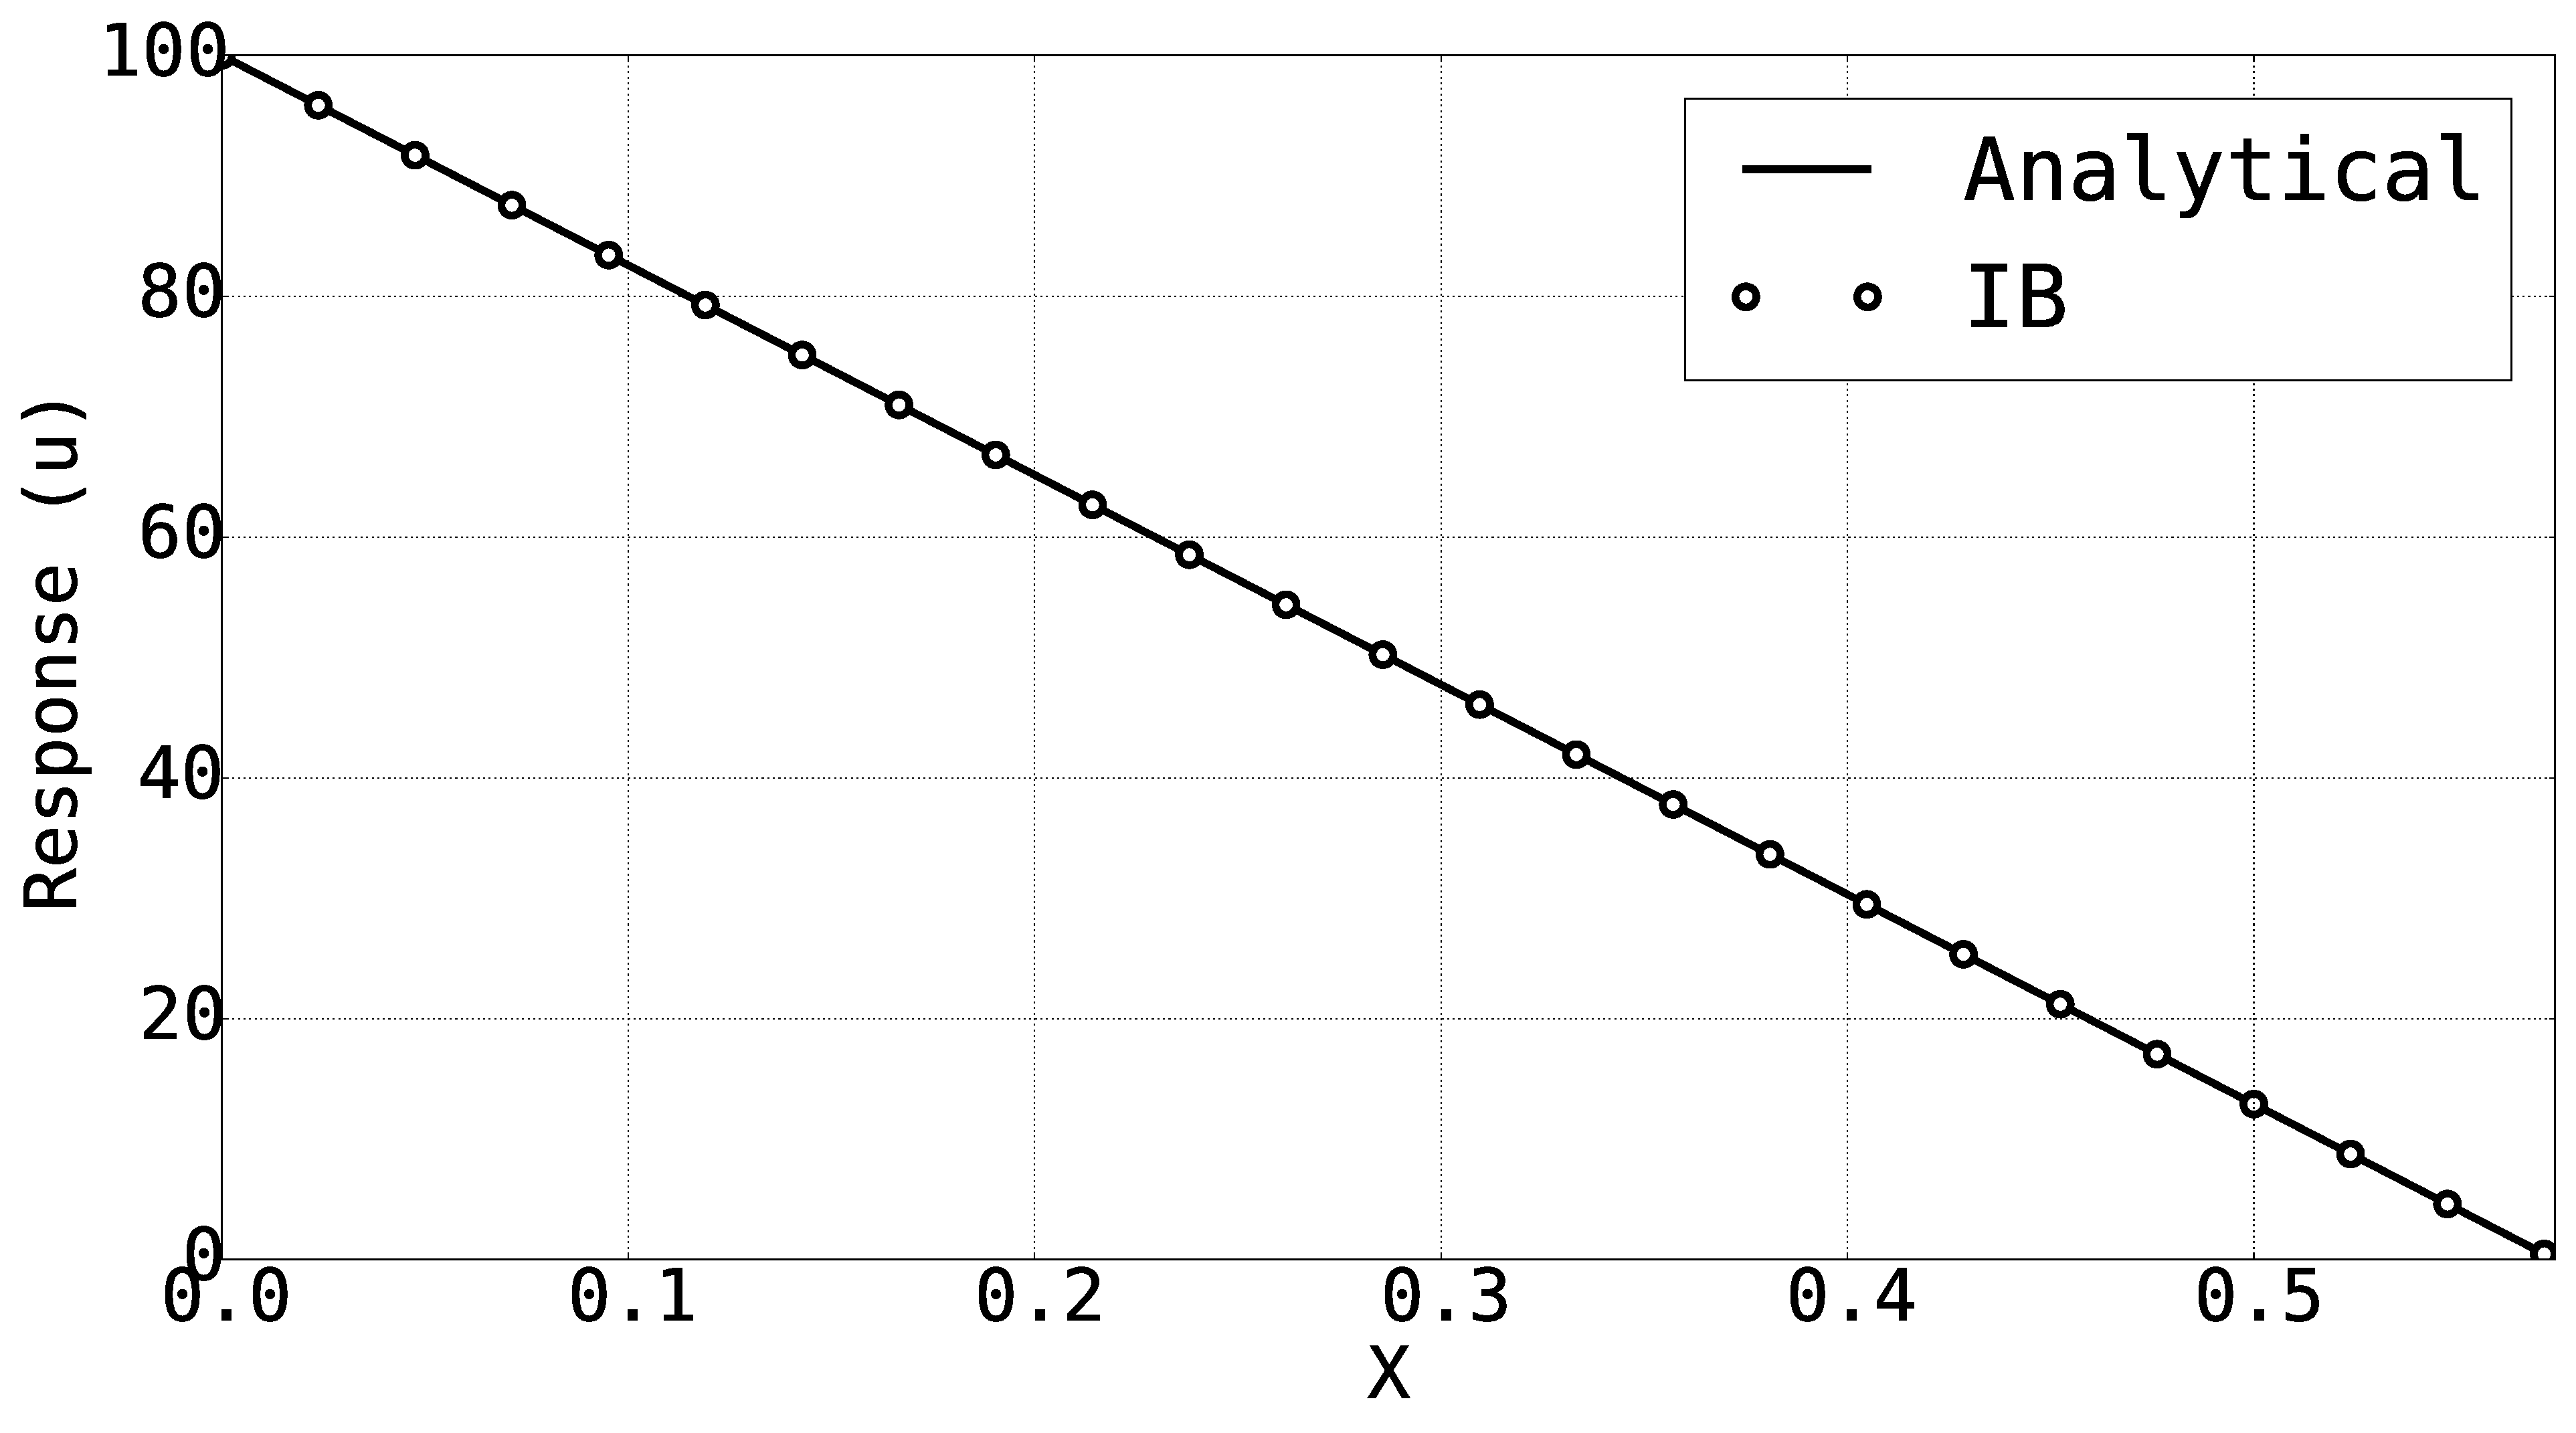
\includegraphics[width=7.0cm]{Chapter_3/figure/indirectForcing_wallVelocity_100.eps}
	}
	\\
	\subfigure[$x_{wall} = 0.612$]
	{
	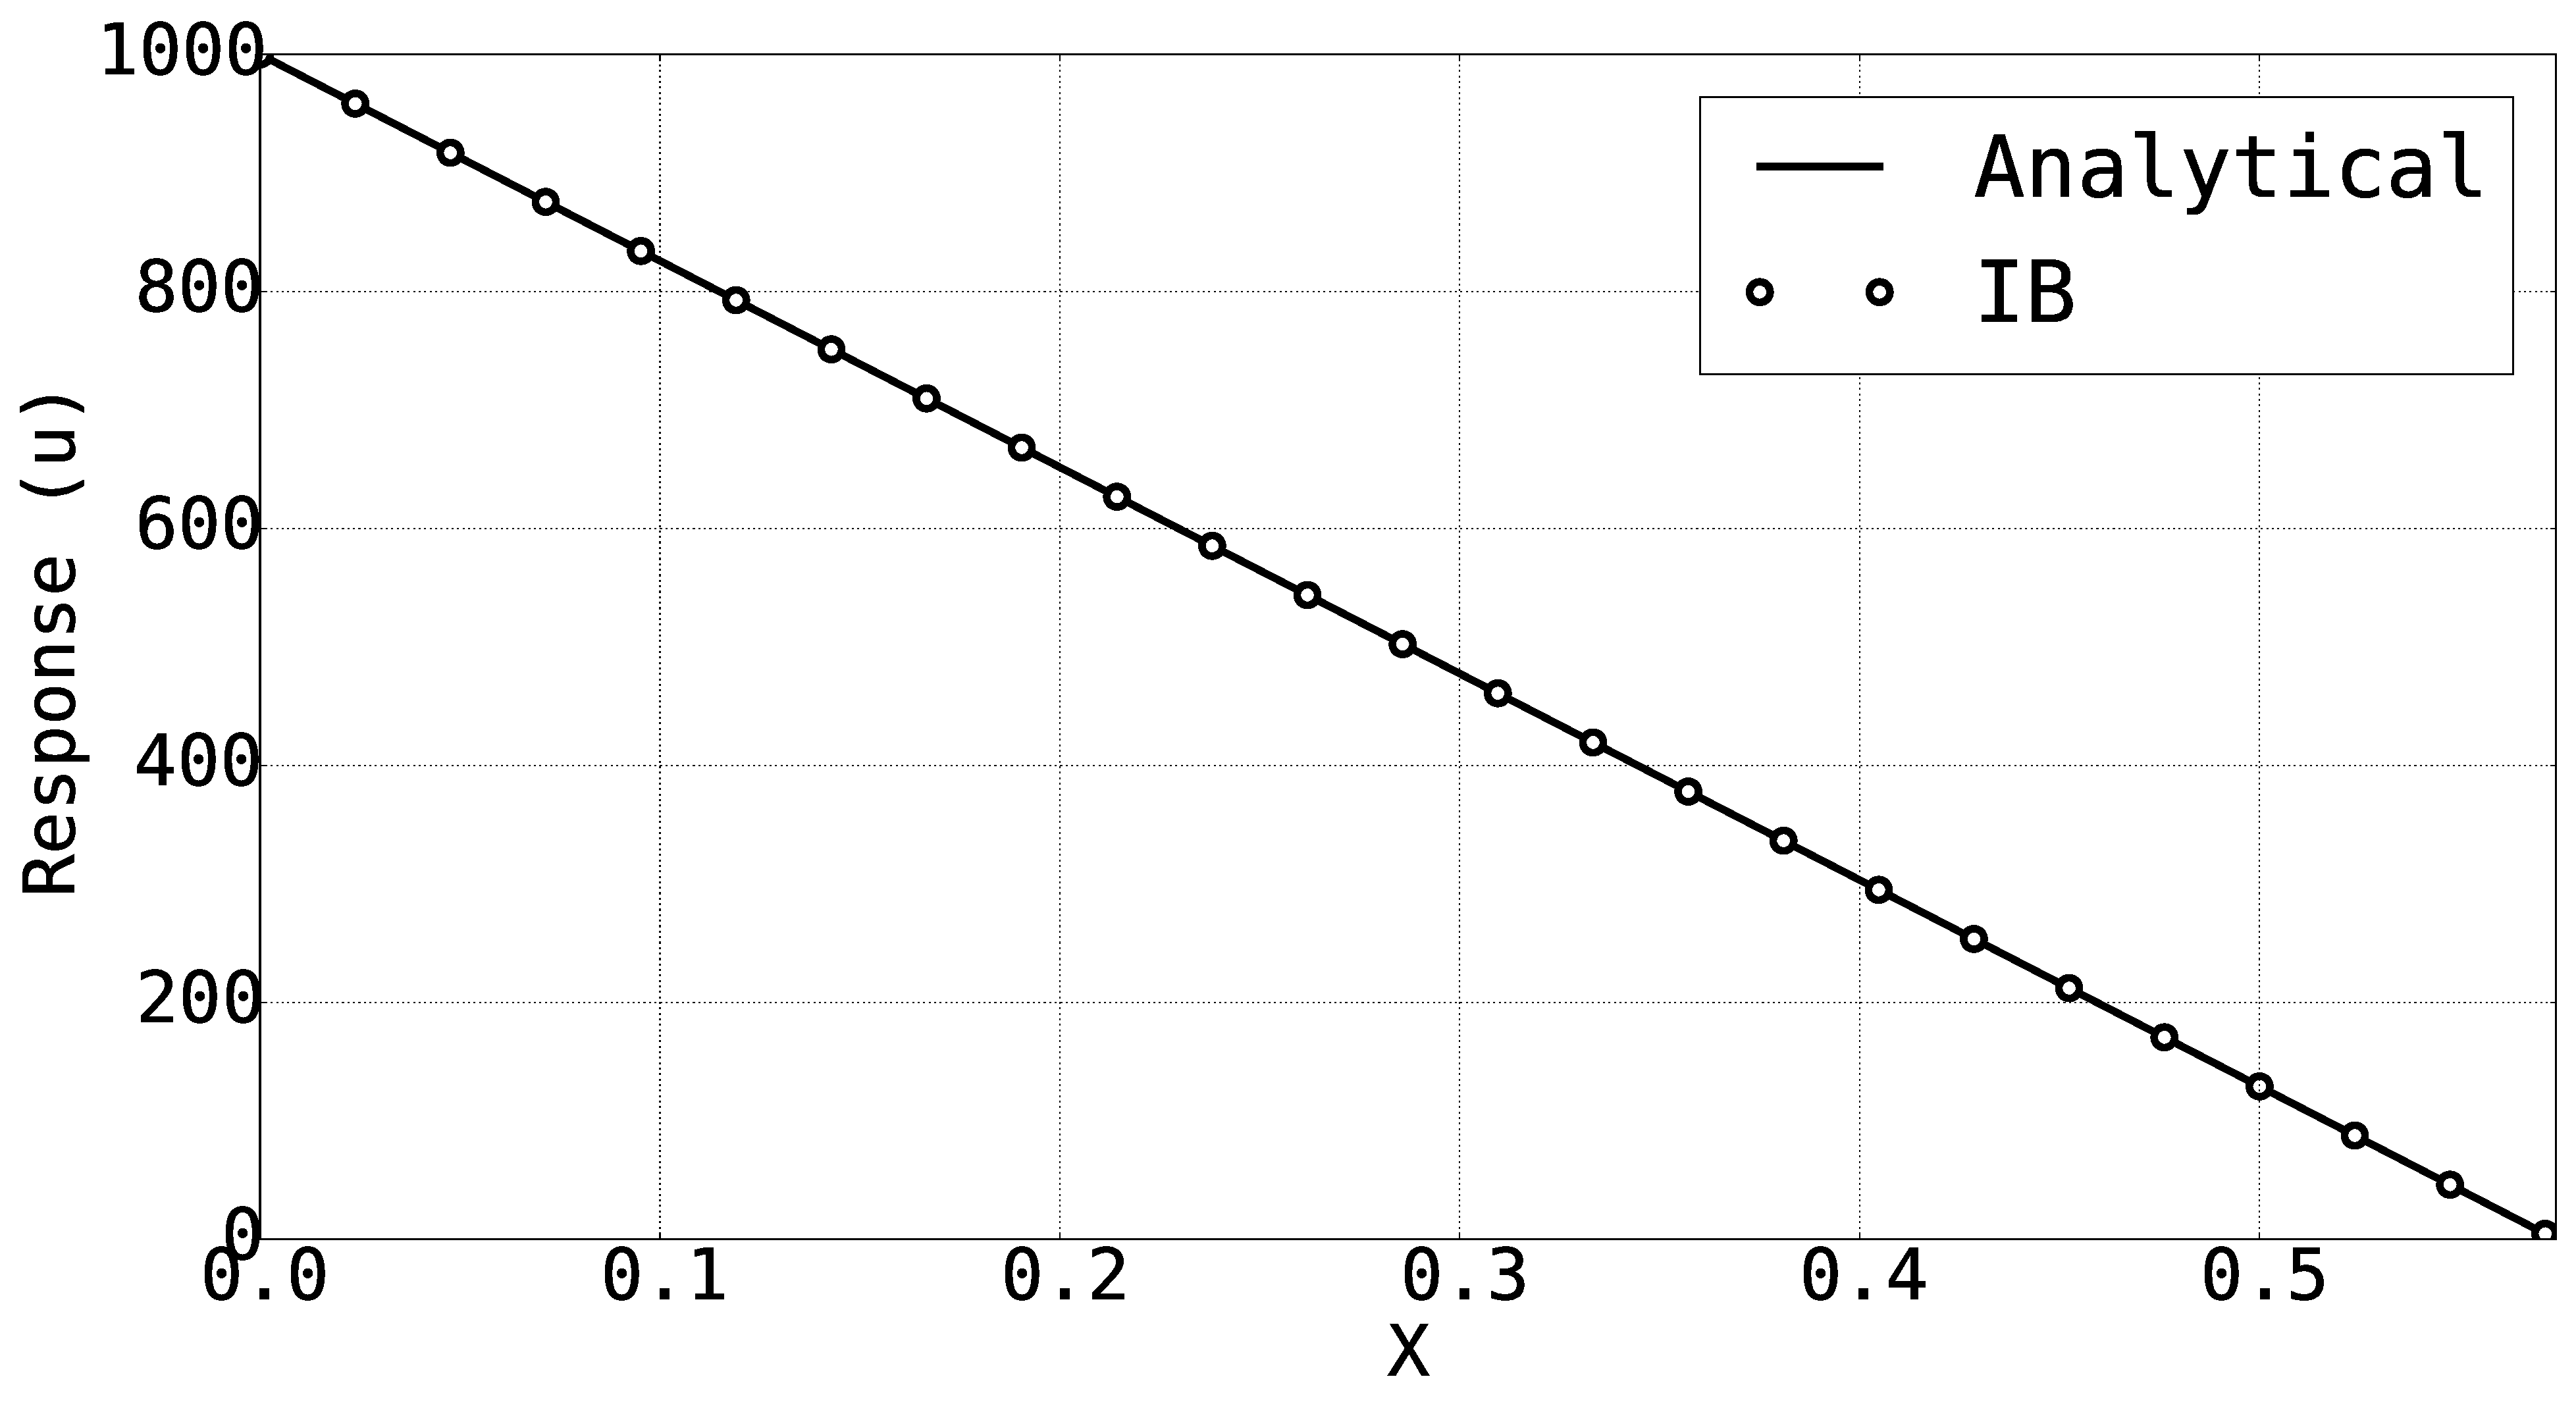
\includegraphics[width=7.0cm]{Chapter_3/figure/indirectForcing_wallVelocity_1000.eps}
	}
	\quad
	\subfigure[$x_{wall} = 0.842$]
	{
	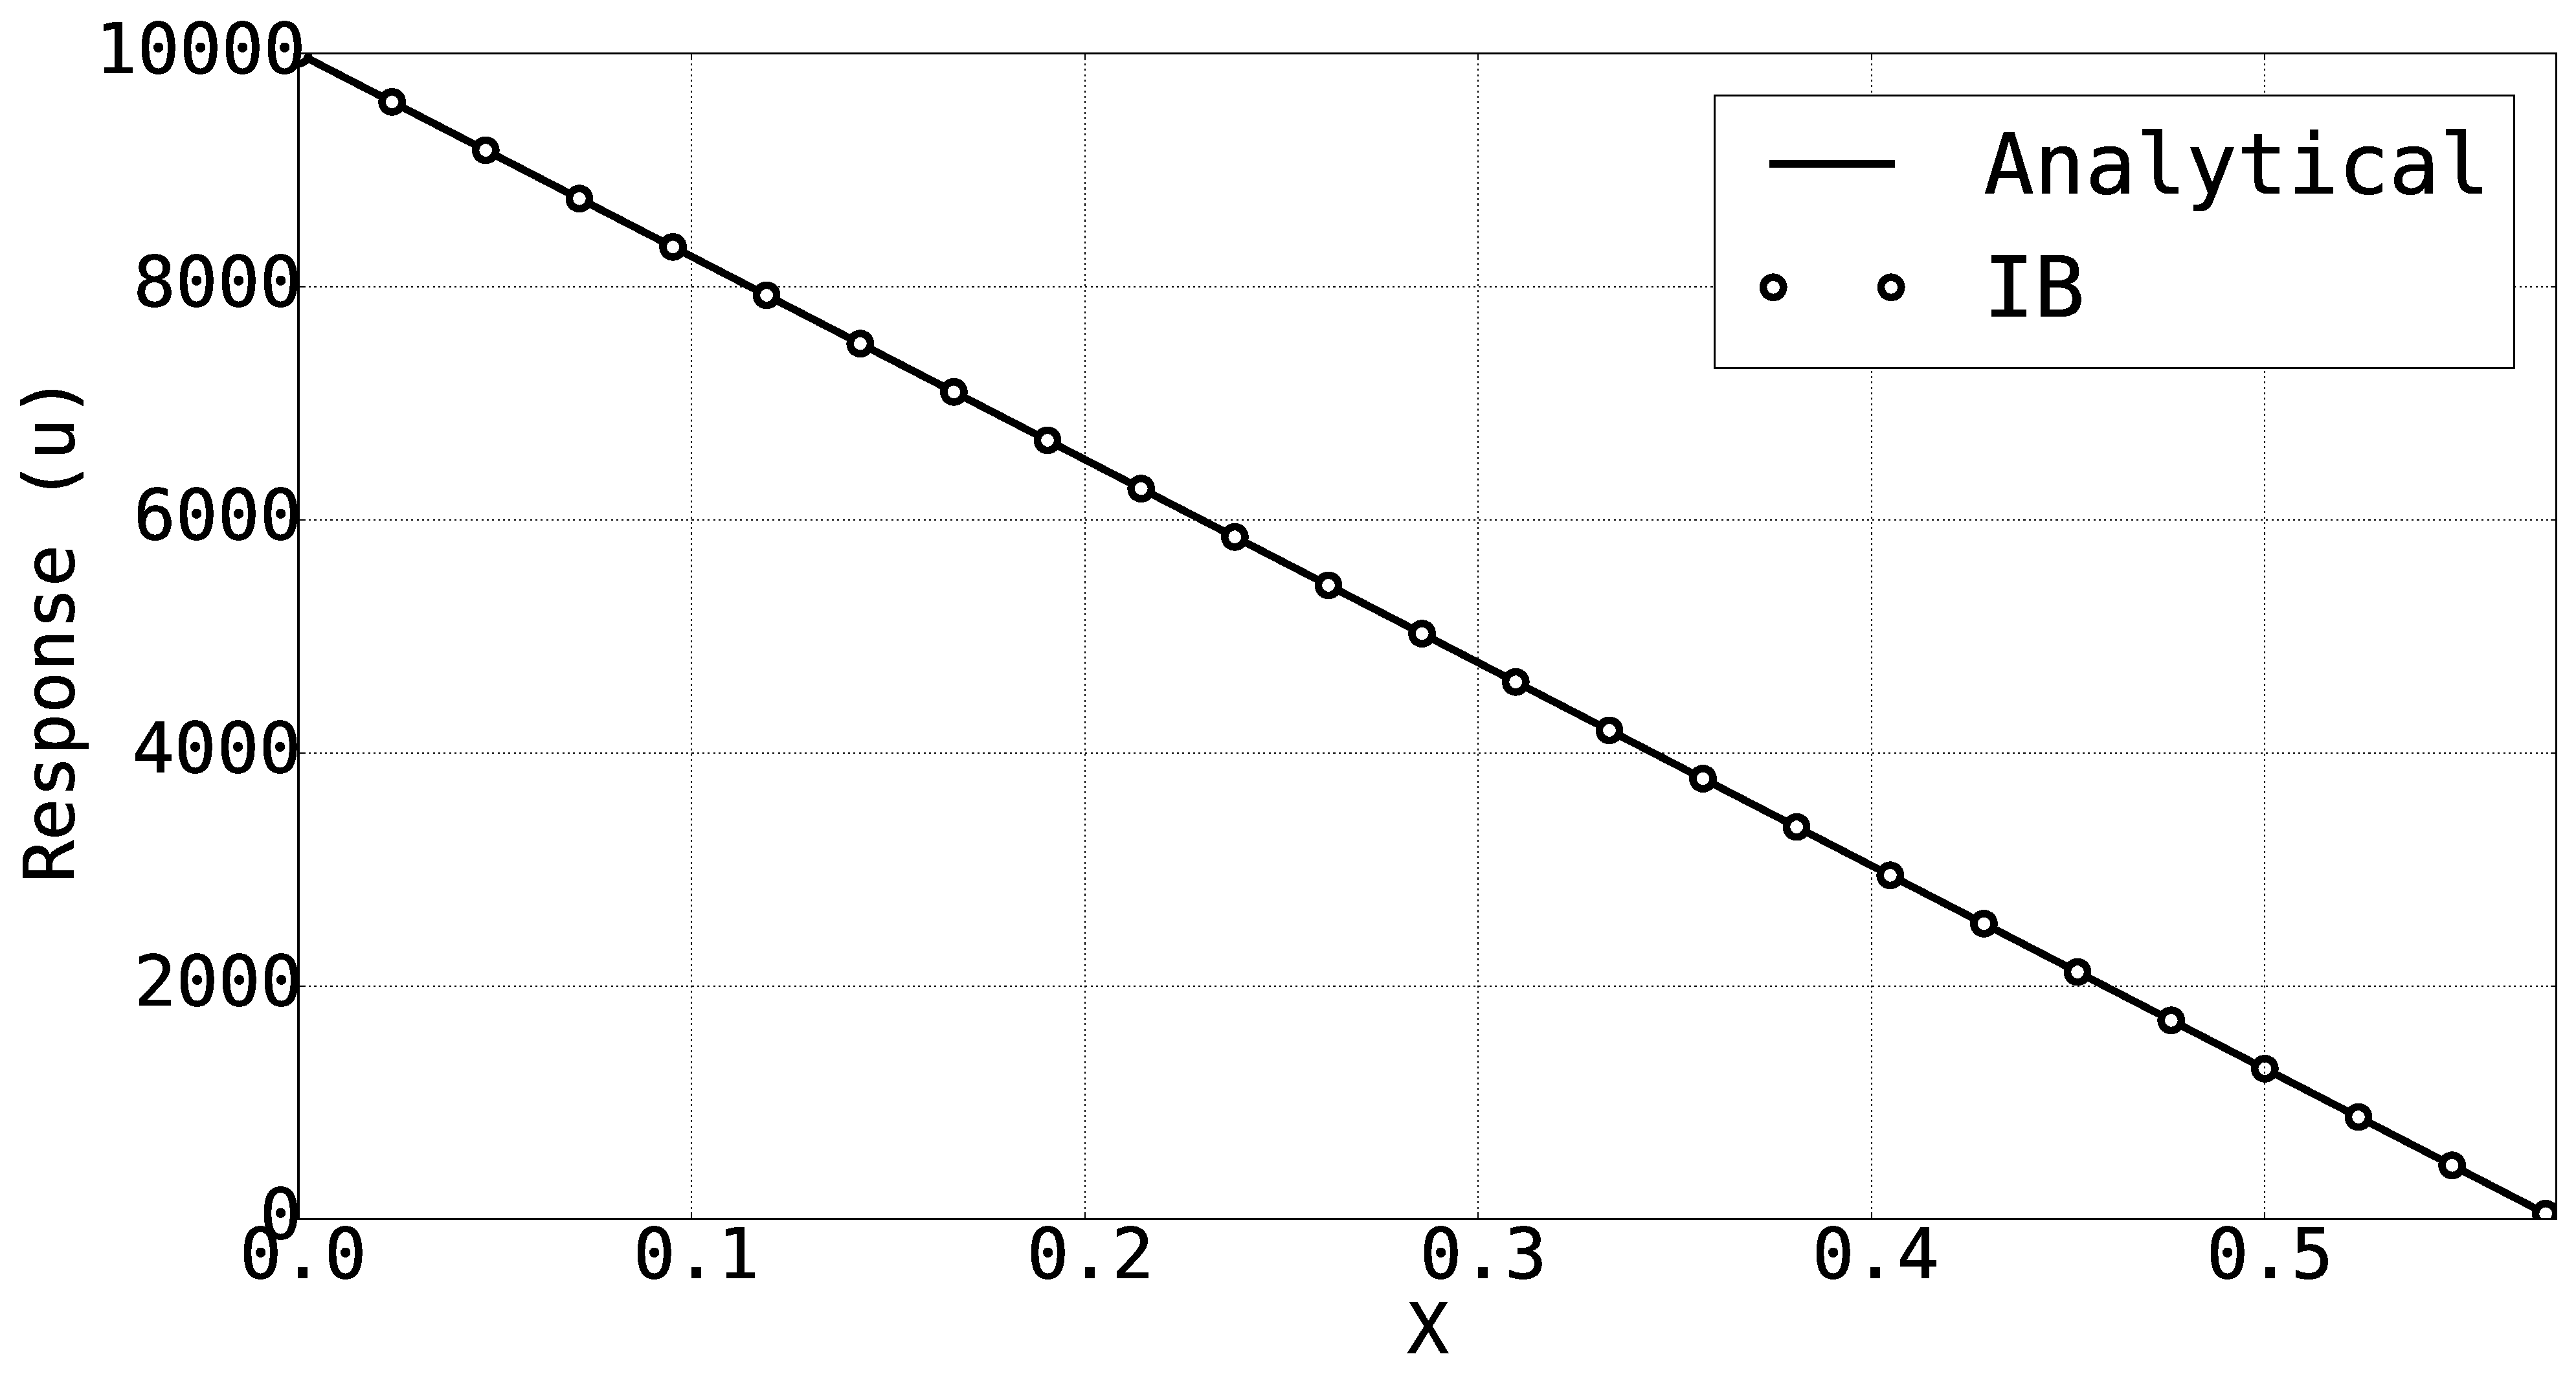
\includegraphics[width=7.0cm]{Chapter_3/figure/indirectForcing_wallVelocity_10000.eps}
	}
	\caption{Comparison between IB and analytical results for different wall velocities.}
	\label{fig:C3_indirectForcing_wallVelocity}
\end{figure}

\begin{table}[H]
\centering
\begin{tabular}{c | c}
	 Wall velocity & RMSE value \\ \hline \hline
	 10 & $1.49 \times 10^{-14}$ \\ \hline
	 100 & $1.52 \times 10^{-14}$ \\ \hline
	 1000 & $1.45 \times 10^{-14}$ \\ \hline
	 10000 & $1.48 \times 10^{-14}$

\end{tabular}
\caption{RMSE value for different wall velocities.}
\label{table:C3_indirectForcing_wallVelocityRSME}
\end{table}

% -.-.-.-.-.-.-.-.-.-.-.-.-.-.-.-.-.-.-.-.-.-.-.-.-.-.-.-.-.-.-.-.-.-
\subsection{Direct forcing method}
In the direct forcing method, the conditions on the immersed boundary are imposed through a set of Ghost cells. These are the cells in the solid region that have at least one neighbour in the fluid domain. For example, the node $\phi$ in Figure \ref{fig:C3_ghostCell} is a ghost cell.

\begin{figure}[H]
	\centering
	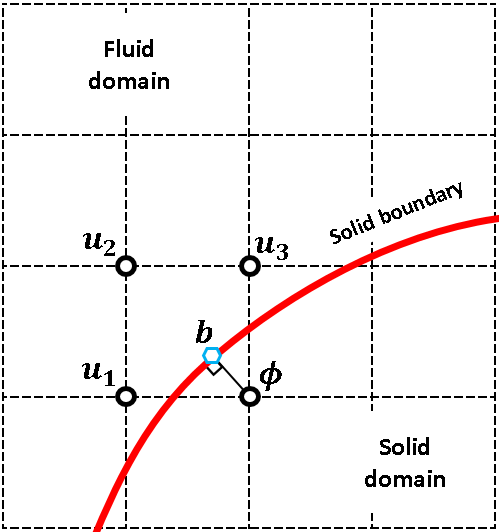
\includegraphics[width=7.00cm]{Chapter_3/figure/discrete_forcing_approach.png}
	\caption{Representation of nodes in the vicinity of an immersed boundary used in the ghost-cell approach.}
	\label{fig:C3_ghostCell}
\end{figure}

For each ghost cell, an interpolation is used to implicitly satisfy the desired value of response on the immersed boundary. The easiest interpolation used is the bilinear interpolation (trilinear in 3D) where the value of $\phi$ can be defined as

\begin{equation}
	\phi = C_1 x_1 x_2 + C_2 x_1 + C_3 x_2 + C_4
\end{equation}

where the four coefficients in above equation is calculated based on the values of flow response at $U_1$, $U_2$, $U_3$ from the solution and the known value at the boundary point $b$. Boundary point $b$, is the normal intercept from the ghost node to the immersed boundary. The linear interpolation is well suited for the laminar flows or for high Reynolds number flows where the gird points are located in the viscous sublayer \cite{iaccarino2003immersed}. For high Reynolds number where higher accuracy is required, higher-order interpolation are used. An example of such interpolations are suggested by Majumdat et al., where they employed a linear interpolation in the tangential direction and quadratic in the normal direction \cite{majumdar2001rans}. 

The ghost cell method, introduce the boundary conditions on the immersed boundary surface directly into the discrete equations. Therefore, the forcing term depends on the discretization process and its practical implementation is not straightforward compared to the continuous forcing approach which is discussed in the next section. The steps for implementing the ghost cell method can be summarized as follows

\begin{enumerate}
	\item Mark computational nodes as fluids, solids, and ghost cells based on their relative location to the boundary
	\item For each of ghost cells, define an interpolation scheme based on the neighbouring nodes
	\item Update the discretized equations for nodes with ghost cell in their boundaries using the interpolation scheme
	\item Solve the resulting equations for the response
	\item Update the interpolation scheme and discrete equations based on the new values
	\item loop until convergence is satisfied
\end{enumerate}

The ghost cell method is applied to the demonstration problem introduced in Section \ref{sec:C3_benchmark_case}. We chose linear interpolation for this problem since the velocities are rather small. looked at the effect of moving wall velocity and the number of nodes on the accuracy of the solution. The IB results are verified using the analytical solution of the problem. We derive the ghost cell method, by discretizing the domain using 6 nodes using central difference method. For demonstration we define the location of wall between nodes $2$ and $3$ as shown in Figure \ref{fig:C3_discretizedGhostCell}. This makes node $3$ the ghost cell for this problem.

\begin{figure}[H]
	\centering
	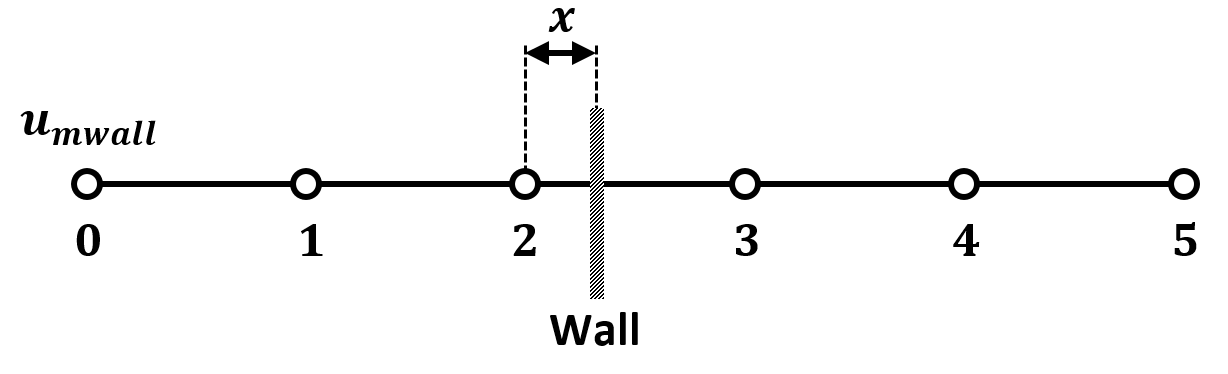
\includegraphics[width=10.00cm]{Chapter_3/figure/ghost_cell_discretization.png}
	\caption{Discretized domain for the ghost cell IB method where the \lq\lq wall\rq\rq\ is represented using hashed box.}
	\label{fig:C3_discretizedGhostCell}
\end{figure}

The solid wall is defined at location $x$ in the local coordinate of the space between nodes $2$ and $3$. By using this coordinate and linear interpolation between nodes $2$ and $3$, the response on the wall is defined as

\begin{equation}
	x u_3 + (1 - x) u_2 = u_{swall}
\end{equation}

where $u_i$ is response at node $i$ and $u_{swall}$ is the predefined velocity at the stationary wall. For this problem, we know that $u_{swall}$ is equal to zero. Therefore, the response at the ghost cell, $u_3$, needs to be equal to the following to ensure zero velocity on the fixed wall.

\begin{equation}\label{eq:C3_ghostCellValue}
	u_3 = -\frac{1 - x}{x} u_2
\end{equation}

The second-order central-difference differential operator for this problem is shown in Equation \eqref{eq:C3_centralDifferenceBefore}. By substituting Equation \eqref{eq:C3_ghostCellValue} in Equation \eqref{eq:C3_centralDifferenceBefore}, we modify the differential operator in a way that it incorporates the effect of solid boundary. This modified operator is shown in Equation \eqref{eq:C3_centralDifferenceAfter}. It should be noted that since the value of $u_3$ is known from Equation \eqref{eq:C3_ghostCellValue}, its corresponding equation is remove from Equation \eqref{eq:C3_centralDifferenceBefore}.

\begin{subequations}
\begin{equation}\label{eq:C3_centralDifferenceBefore}
	L = 
	\begin{bmatrix}
	1 & -2 & 1 & 0 & 0 & 0 \\
	0 & 1 & -2 & 1 & 0 & 0 \\
	0 & 0 & 1 & -2 & 1 & 0 \\
	0 & 0 & 0 & 1 & -2 & 1
	\end{bmatrix} \quad \text{:original operator}
\end{equation}
\begin{equation}\label{eq:C3_centralDifferenceAfter}
	L' = 
	\begin{bmatrix}
	1 & -2 & 1 & 0 & 0 & 0 \\
	0 & 1 & -2-(1-x)/x & 0 & 0 & 0 \\
	0 & 0 & 1+2(1-x)/x & 0 & 1 & 0 \\
	0 & 0 & -(1-x)/x & 0 & -2 & 1
	\end{bmatrix} \quad \text{:modified operator}
\end{equation}
\end{subequations}

The differential operator of Equation \eqref{eq:C3_centralDifferenceAfter} needs to be updated based on the new location of wall. This may cause a different column to become zero. As a results, we need to know the discretization technique used in solving the governing equations in order to implement the ghost method method. This is not usually possible for the commercial packages.

The Euler method is used for time integration of the discrete equations. In the discrete form, this is written as shown in Equation \eqref{eq:C3_euelrMethodBefore}. The time integration is also need to be modified to incorporate the effect of the ghost cell. This is done by incorporating the known value of ghost cell in the time integration as shown in Equation \eqref{eq:C3_euelrMethodAfter}.

\begin{subequations}
\begin{equation}\label{eq:C3_euelrMethodBefore}
	\begin{bmatrix}
	1 & 0 & 0 & 0 \\
	0 & 1 & 0 & 0 \\
	0 & 0 & 1 & 0 \\
	0 & 0 & 0 & 1
	\end{bmatrix}
	\begin{bmatrix}
	u_1^{n+1} \\
	u_2^{n+1} \\
	u_3^{n+1} \\
	u_4^{n+1}
	\end{bmatrix}
	=
	\begin{bmatrix}
	1 & 0 & 0 & 0 \\
	0 & 1 & 0 & 0 \\
	0 & 0 & 1 & 0 \\
	0 & 0 & 0 & 1
	\end{bmatrix}
	\begin{bmatrix}
	u_1^{n} \\
	u_2^{n} \\
	u_3^{n} \\
	u_4^{n}
	\end{bmatrix}
	+ 
	\Delta t L \mathbf{u}^n
\end{equation}
\begin{equation}\label{eq:C3_euelrMethodAfter}
	\begin{bmatrix}
	1 & 0 & 0 & 0 \\
	0 & 1 & 0 & 0 \\
	0 & 0 & 1 & 0 \\
	0 & 0 & 0 & 1
	\end{bmatrix}
	\begin{bmatrix}
	u_1^{n+1} \\
	u_2^{n+1} \\
	u_3^{n+1} \\
	u_4^{n+1}
	\end{bmatrix}
	=
	\begin{bmatrix}
	1 & 0 & 0 & 0 \\
	0 & 1 & 0 & 0 \\
	0 & -(1-x)/x & 0 & 0 \\
	0 & 0 & 0 & 1
	\end{bmatrix}
	\begin{bmatrix}
	u_1^{n} \\
	u_2^{n} \\
	u_3^{n} \\
	u_4^{n}
	\end{bmatrix}
	+ 
	\Delta t L' \mathbf{u}^n
\end{equation}
\end{subequations}

where $L'$ is the modified differential operator of Equation \eqref{eq:C3_centralDifferenceAfter}. It is clear that excessive modification of the discrete solver is required for implementation of the immersed boundary. This discretization method is applied to the benchmark case, where the effect of node number, location of the stationary wall, and the wall velocity on the solution accuracy are investigated.

For the first case, we look at the effect of node number. We choose the length of domain as $1m$ with the wall located at $x_{wall} = 0.6541$. The time step is selected as $0.1$ with the moving wall velocity as $10 m/s$. The node numbers at selected as $11$, $41$, $81$, and $161$ for this purpose. We compared the accuracy of the solution by comparing it to the analytical result. We chose the normalized root mean square error to compared the analytical and IB results. This is defined as follows.

\begin{equation*}
	NRMSE = \dfrac{\sqrt{\dfrac{\sum_{n=1}{N} \left( \hat{y}_n - y \right)^2}{n}}}{y_{max} - y_{min}}
\end{equation*}

where $\hat{y}_t$ is the predicted value, $y$ is the true value, and $n$ is the number data points. Normalizing by $y_{max} - y_{min}$ enables us to compare models with different scales. This is especially useful when compared the results for different wall velocities.

As shown in Figure \ref{fig:C3_ghostCell_nodeNumber} and \ref{table:C3_ghostCell_nodeNumber_RMSE}, the number of nodes does not affect the solution accuracy. It is possible to get good accuracies even with low number of nodes. This is because the boundary condition is exactly satisfied at the wall location due to the ghost cell.

\begin{figure}[H]
	\centering
	\subfigure[N = 11]
	{
	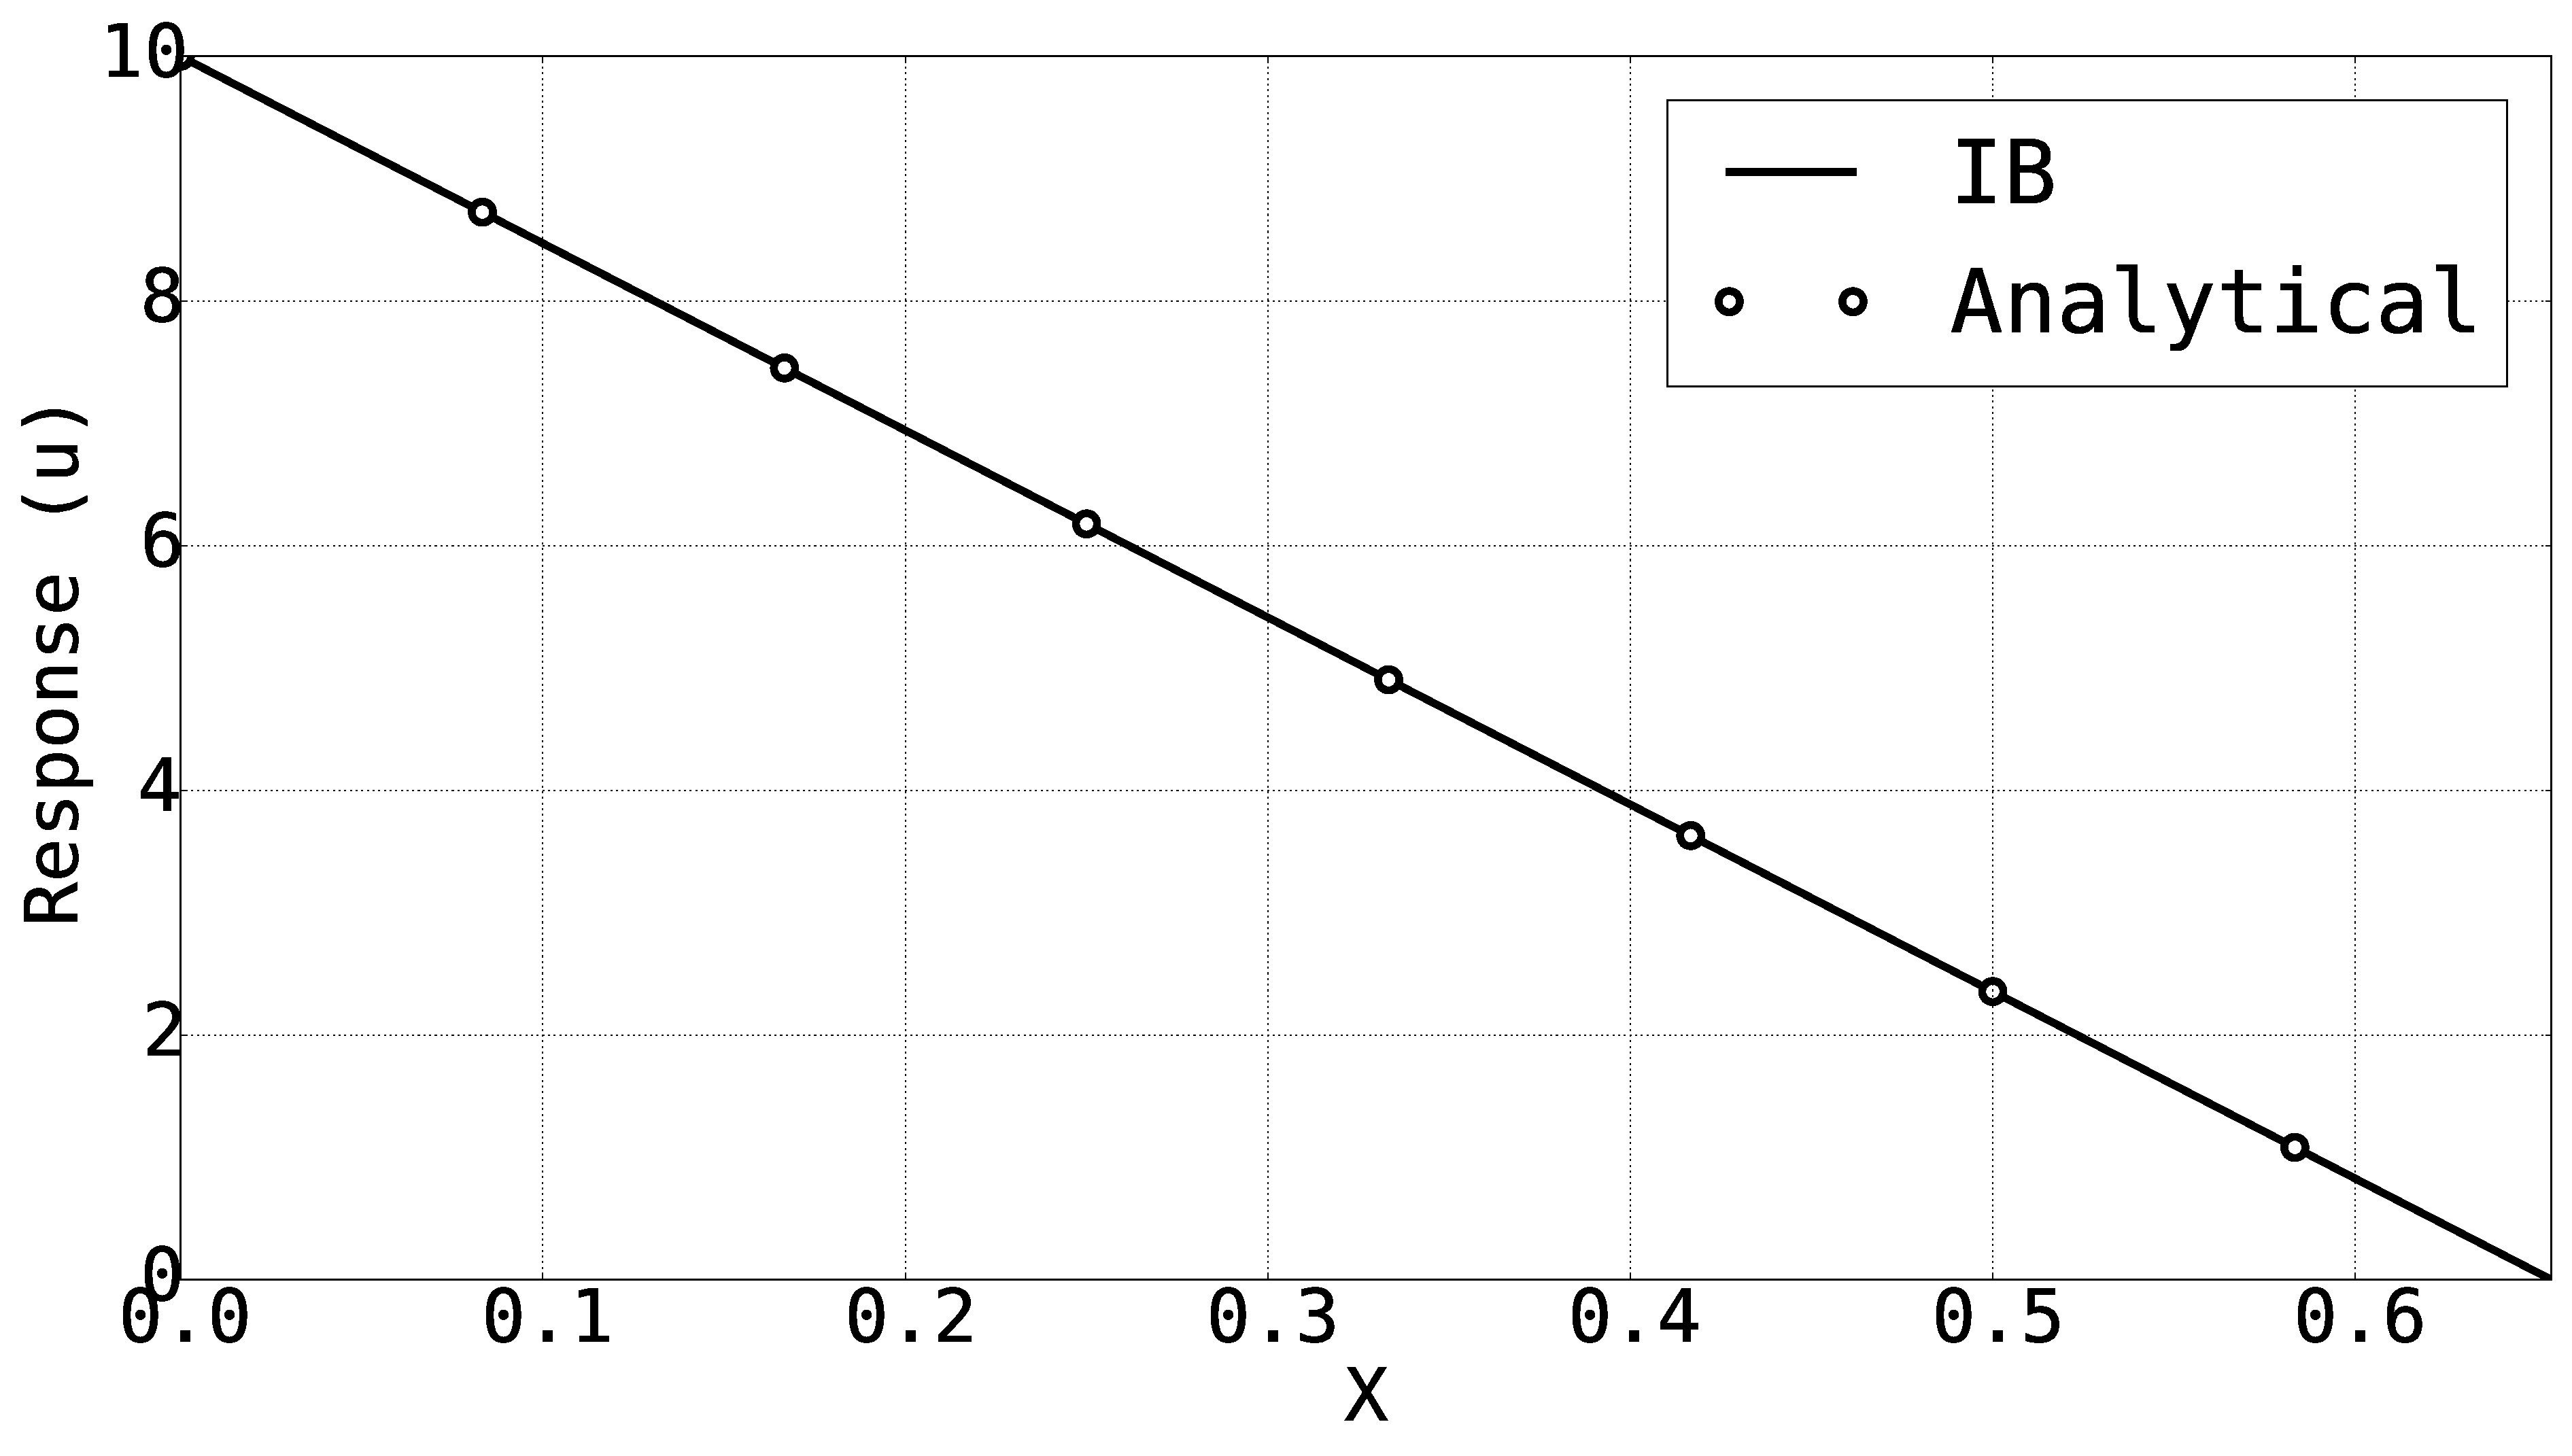
\includegraphics[width=7.0cm]{Chapter_3/figure/ghostCell_nodeNumber_11.eps}
	}
	\quad
	\subfigure[N = 41]
	{
	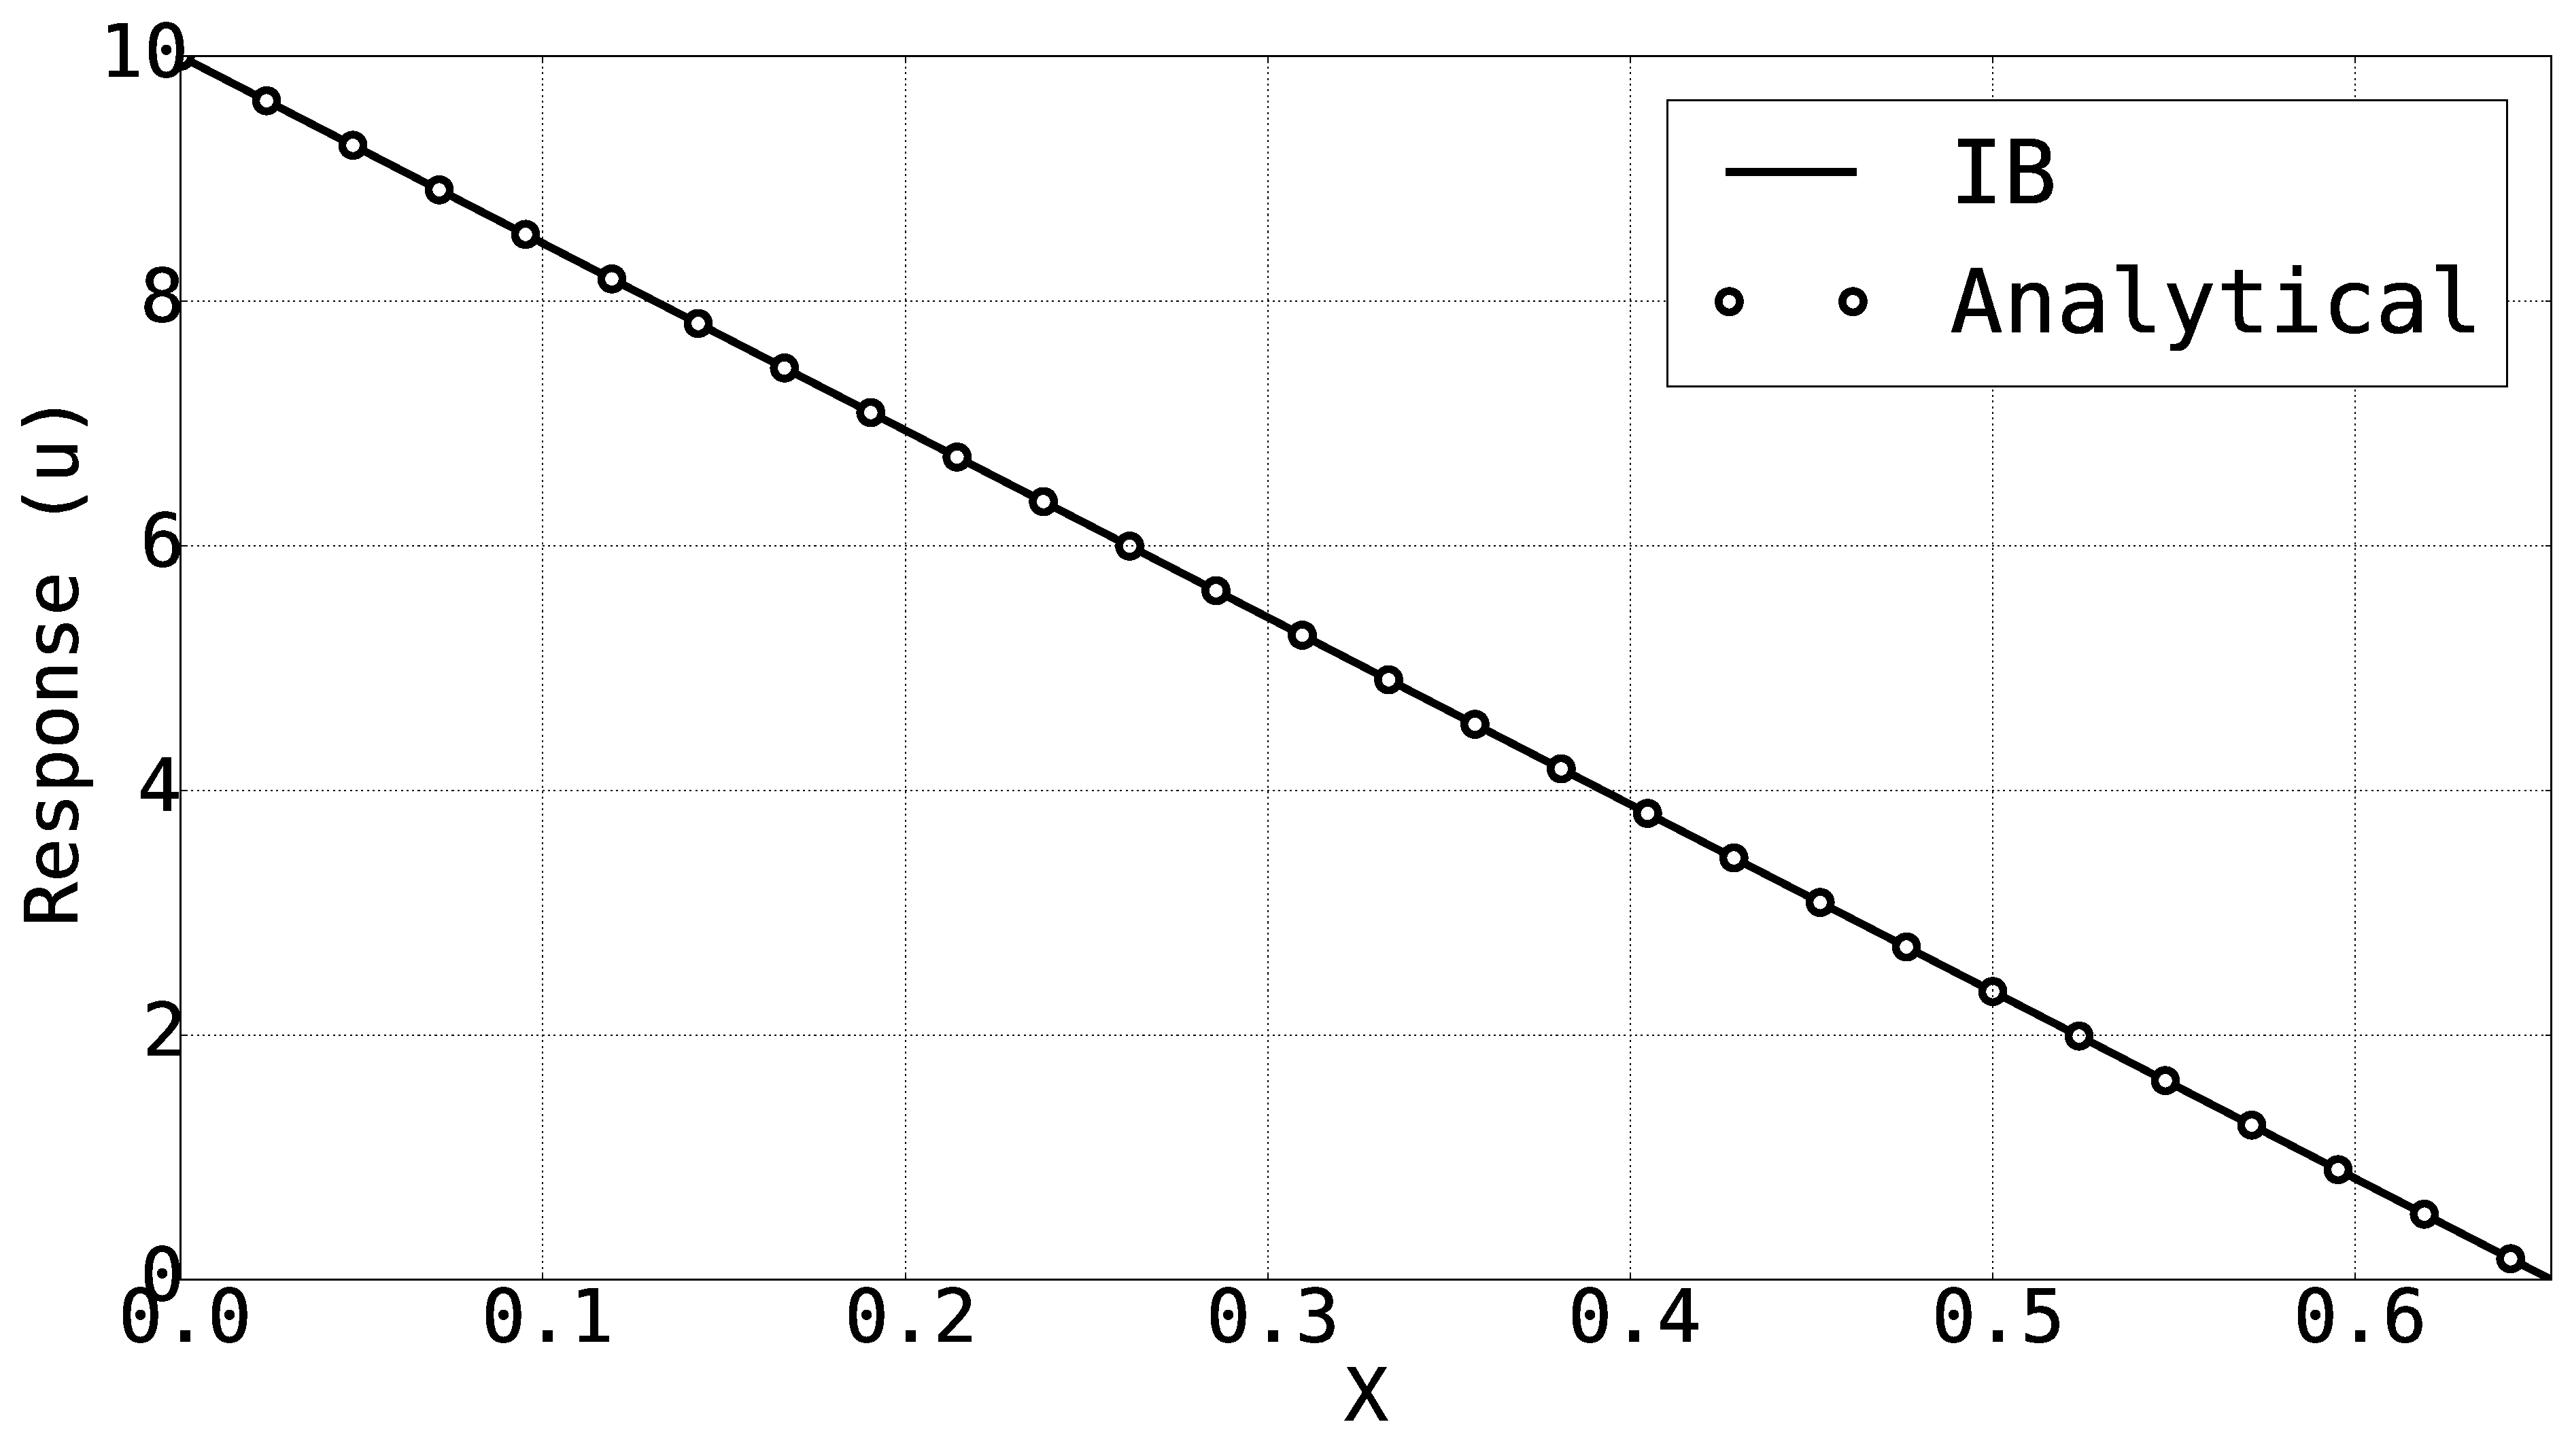
\includegraphics[width=7.0cm]{Chapter_3/figure/ghostCell_nodeNumber_41.eps}
	}
	\\
	\subfigure[N = 81]
	{
	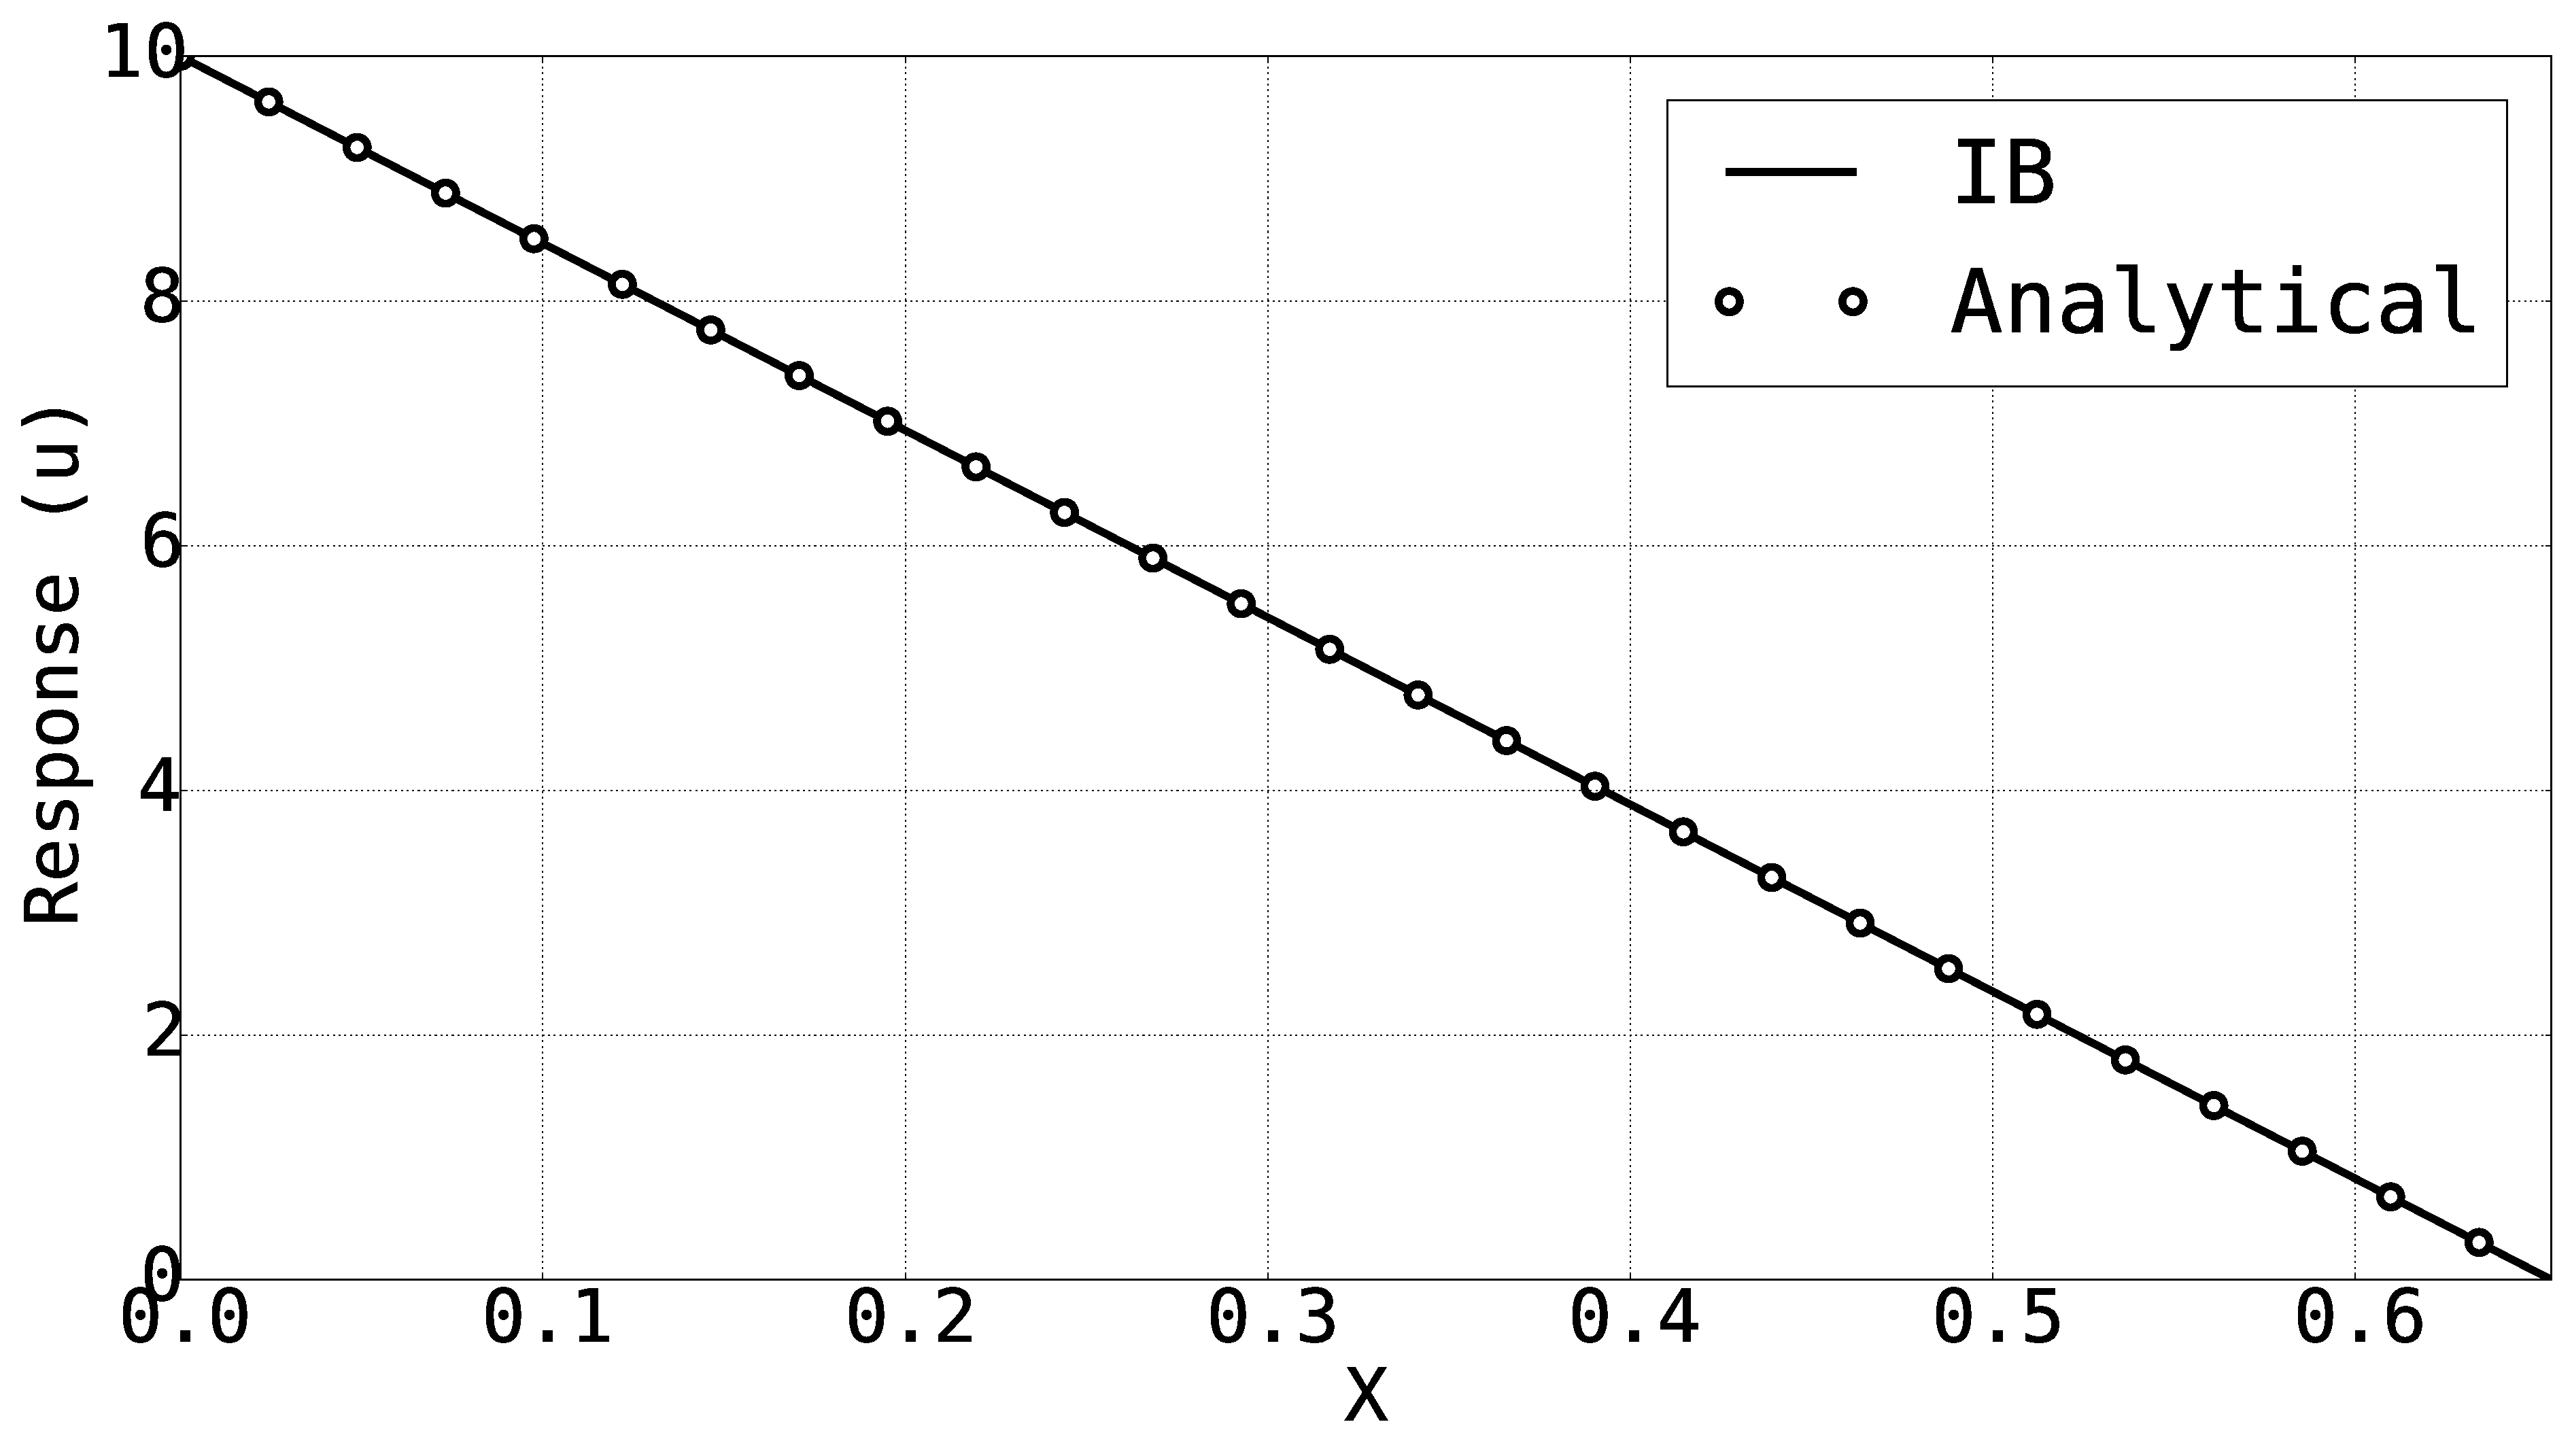
\includegraphics[width=7.0cm]{Chapter_3/figure/ghostCell_nodeNumber_81.eps}
	}
	\quad
	\subfigure[N = 161]
	{
	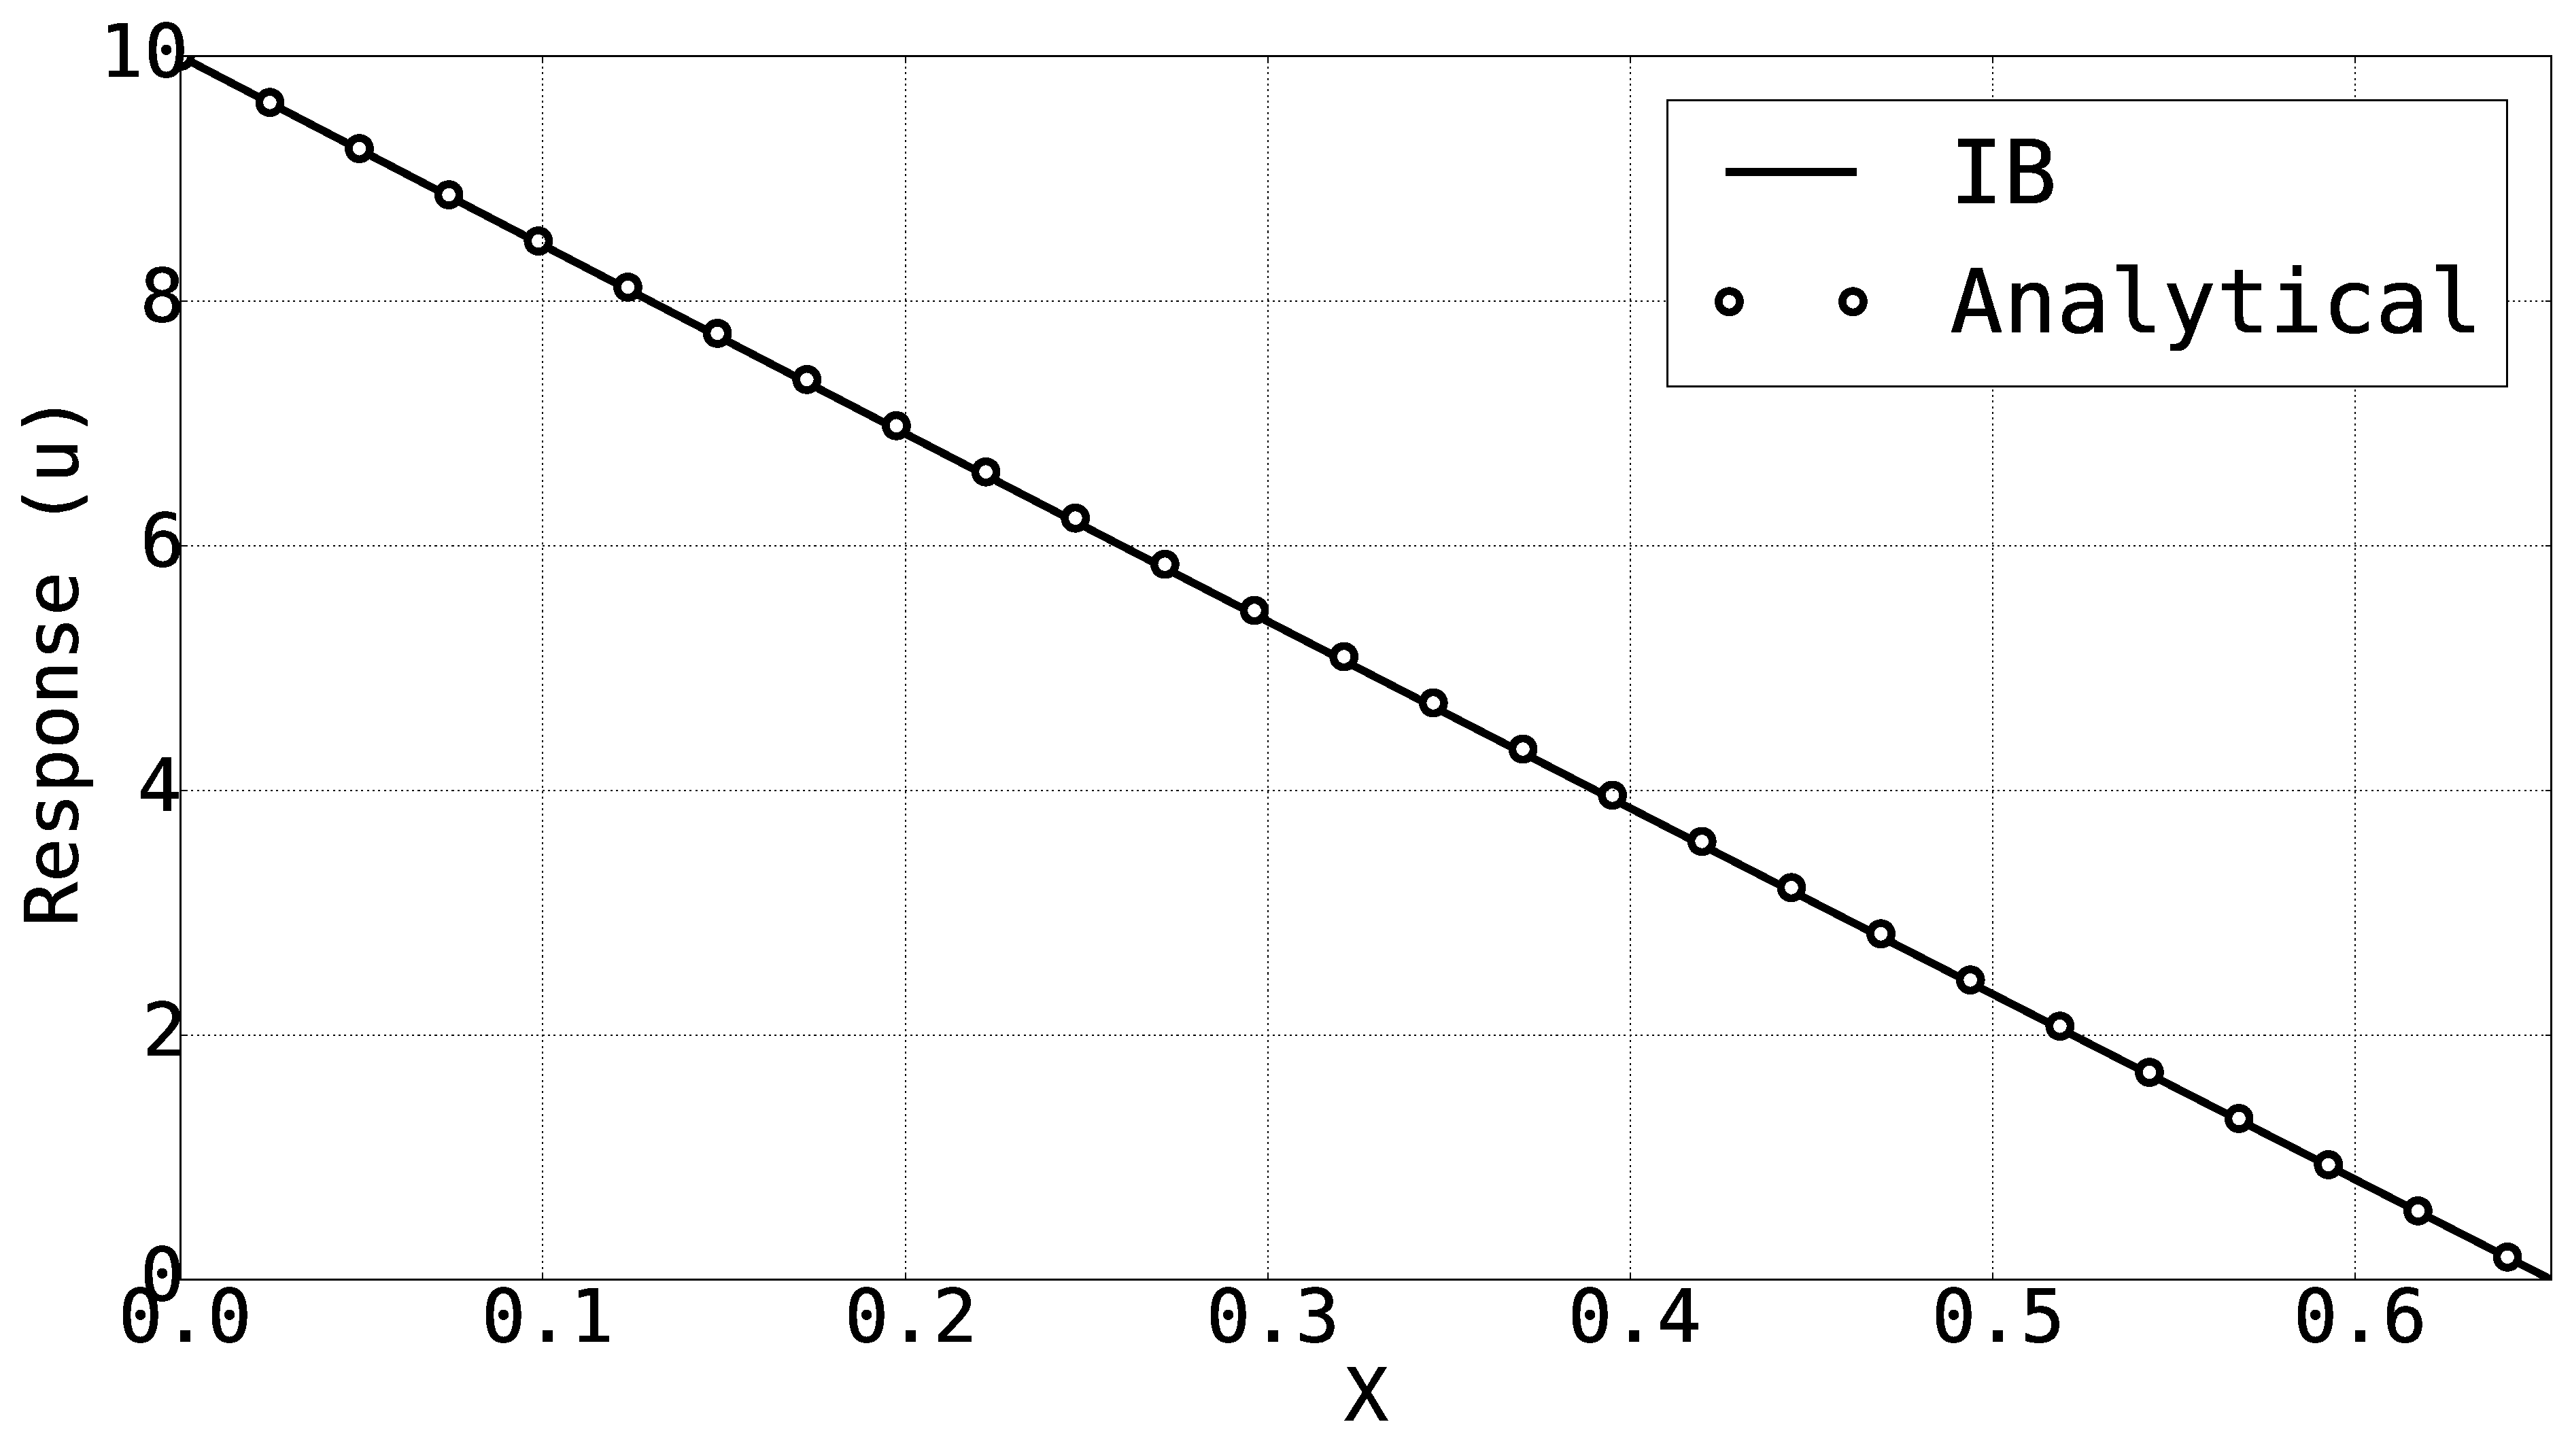
\includegraphics[width=7.0cm]{Chapter_3/figure/ghostCell_nodeNumber_161.eps}
	}
	\caption{Comparison between IB and analytical results for different node numbers.}
	\label{fig:C3_ghostCell_nodeNumber}
\end{figure}

\begin{table}[H]
\centering
\begin{tabular}{c | c}
	 Node number & RMSE value \\ \hline \hline
	 11 & $1.49 \times 10^{-15}$ \\ \hline
	 41 & $2.08 \times 10^{-15}$ \\ \hline
	 81 & $4.19 \times 10^{-10}$ \\ \hline
	 161 & $9.94 \times 10^{-10}$ \\
\end{tabular}
\caption{RMSE value for different node numbers.}
\label{table:C3_ghostCell_nodeNumber_RMSE}
\end{table}

We solved the same problem but by fixing the number of nodes to $41$ and changing the location of fixed bar to see its effect of the solution. The wall is defined at $0.124$, $0.379$, $0.723$, $0.936$ where none of these location coincide with the computational nodes. As shown in Figure \ref{fig:C3_ghostCell_wallLocation} and Table \ref{table:C3_ghostCell_wallLocation_RMSE}, the solution accuracy is not affected by wall location as well.

\begin{figure}[H]
	\centering
	\subfigure[N = 11]
	{
	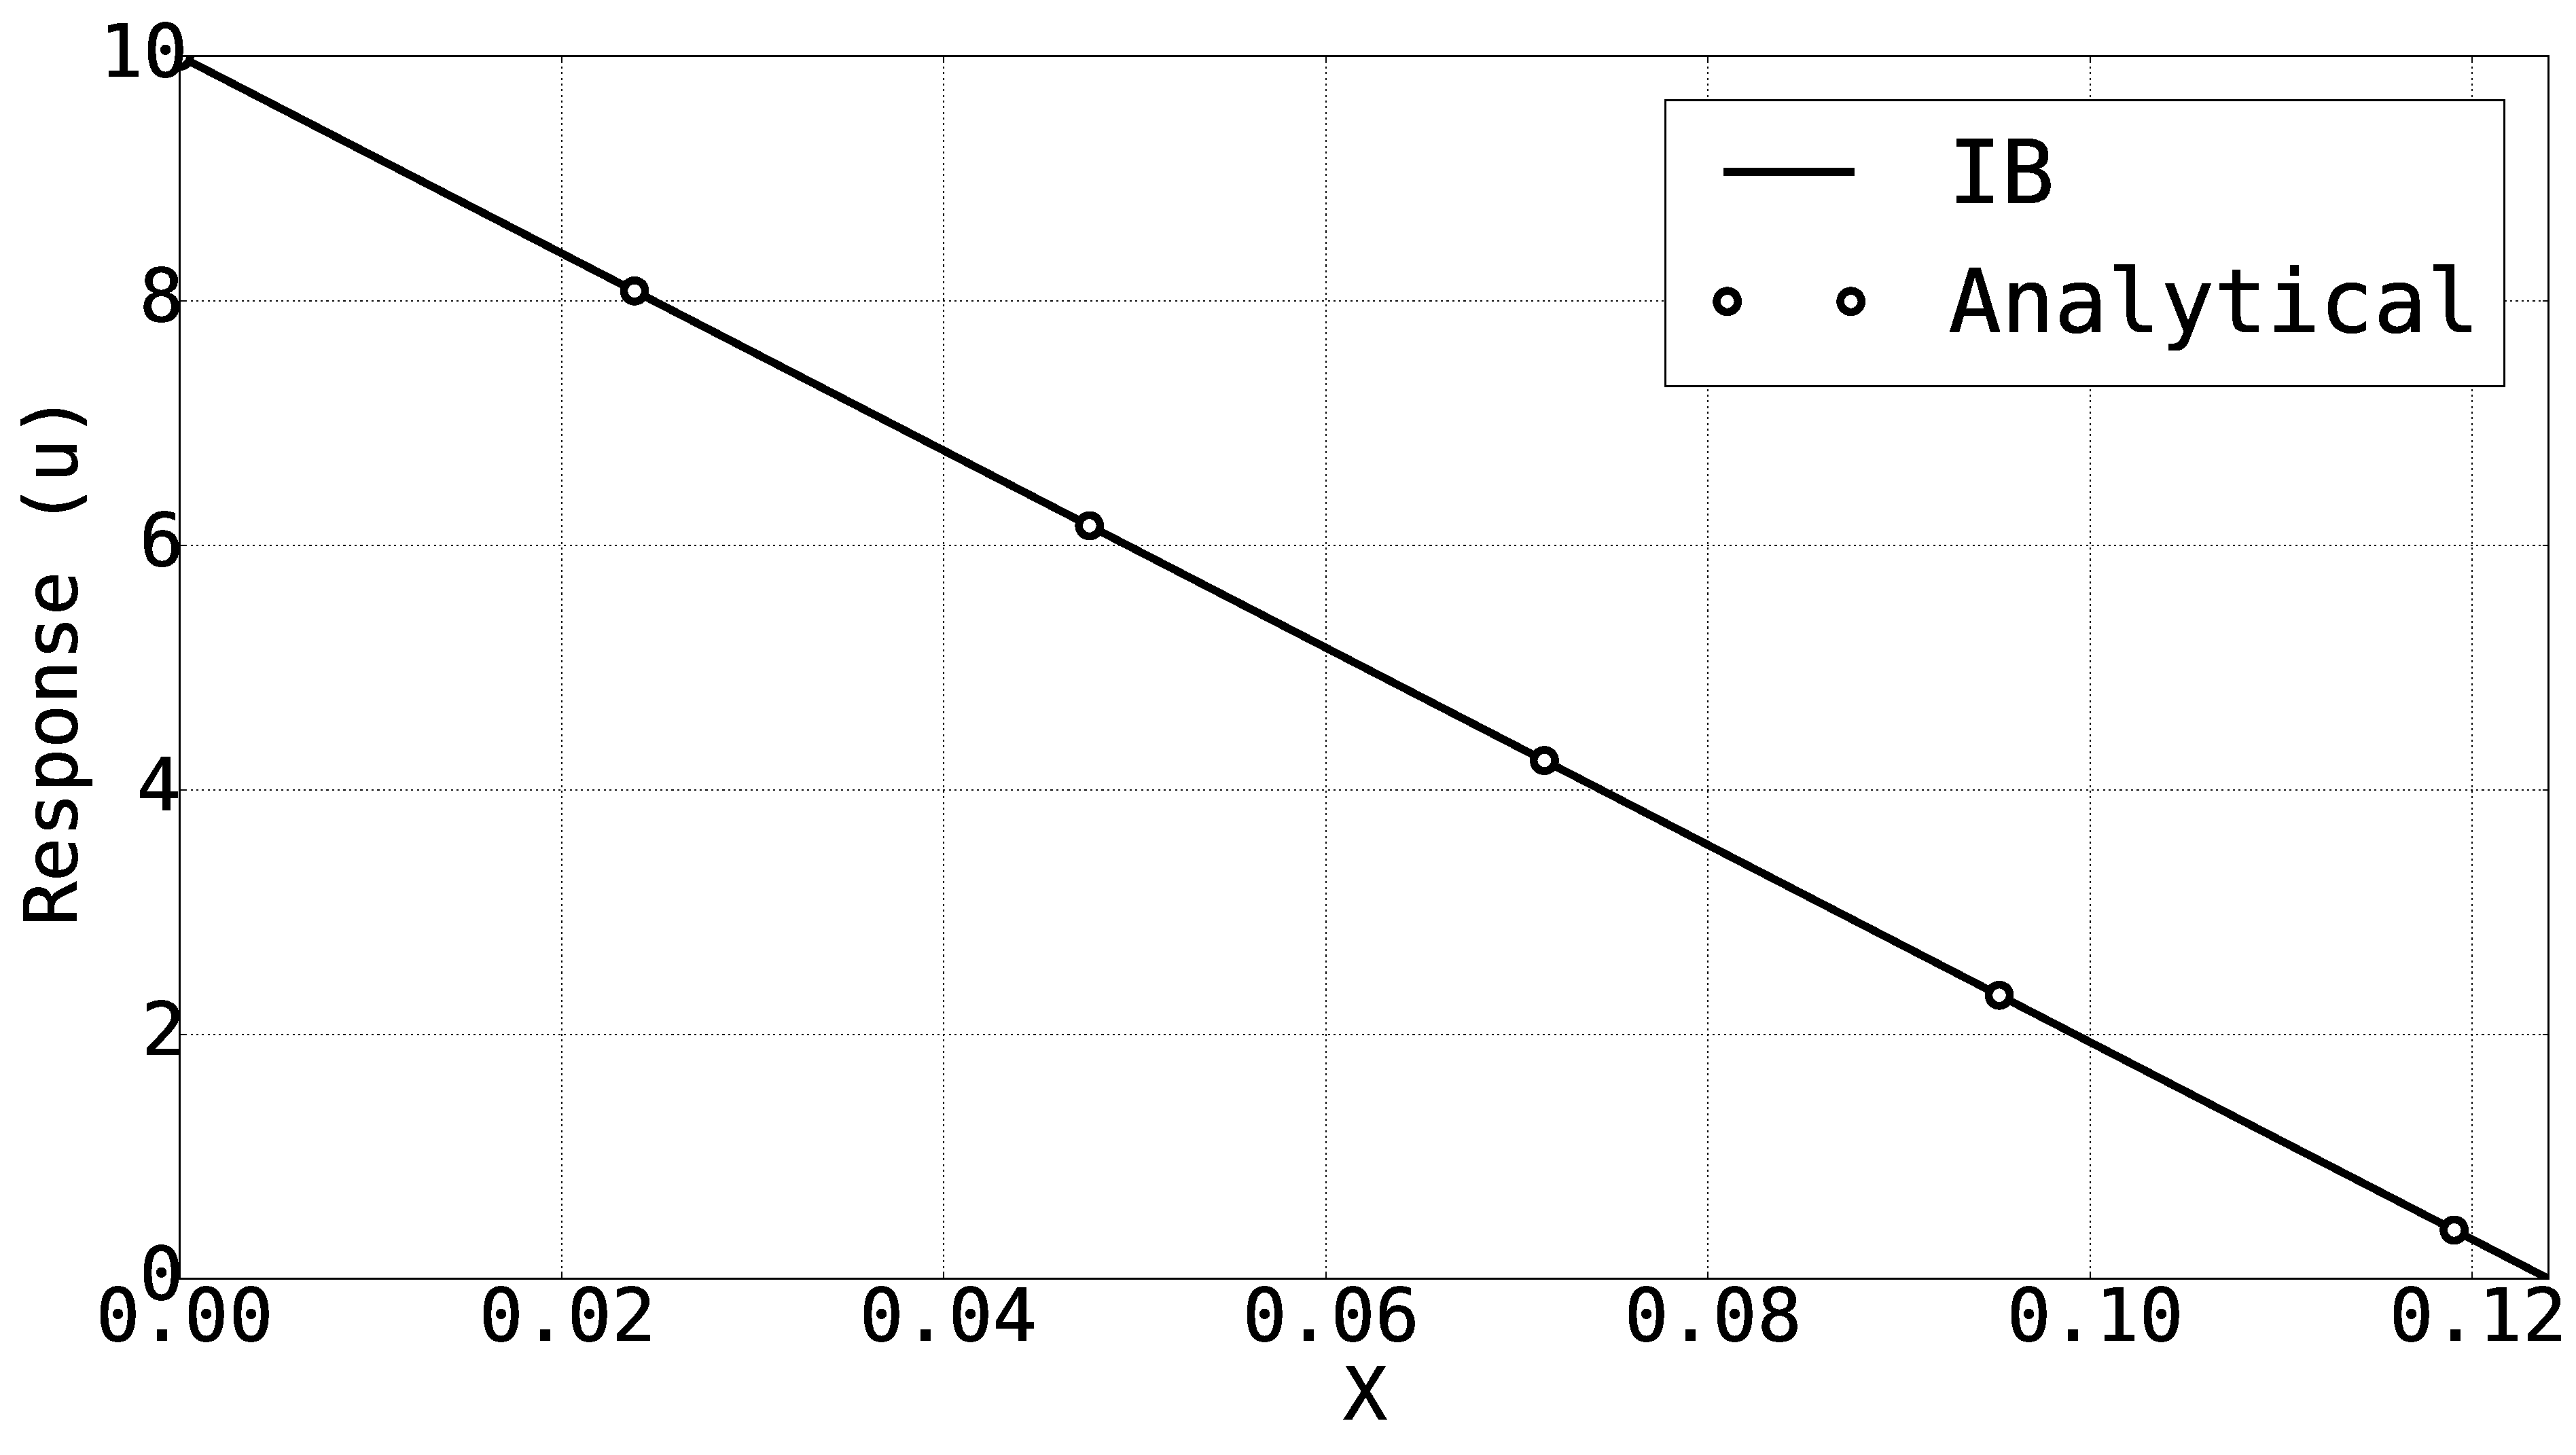
\includegraphics[width=7.0cm]{Chapter_3/figure/ghostCell_wallLocation_124.eps}
	}
	\quad
	\subfigure[N = 41]
	{
	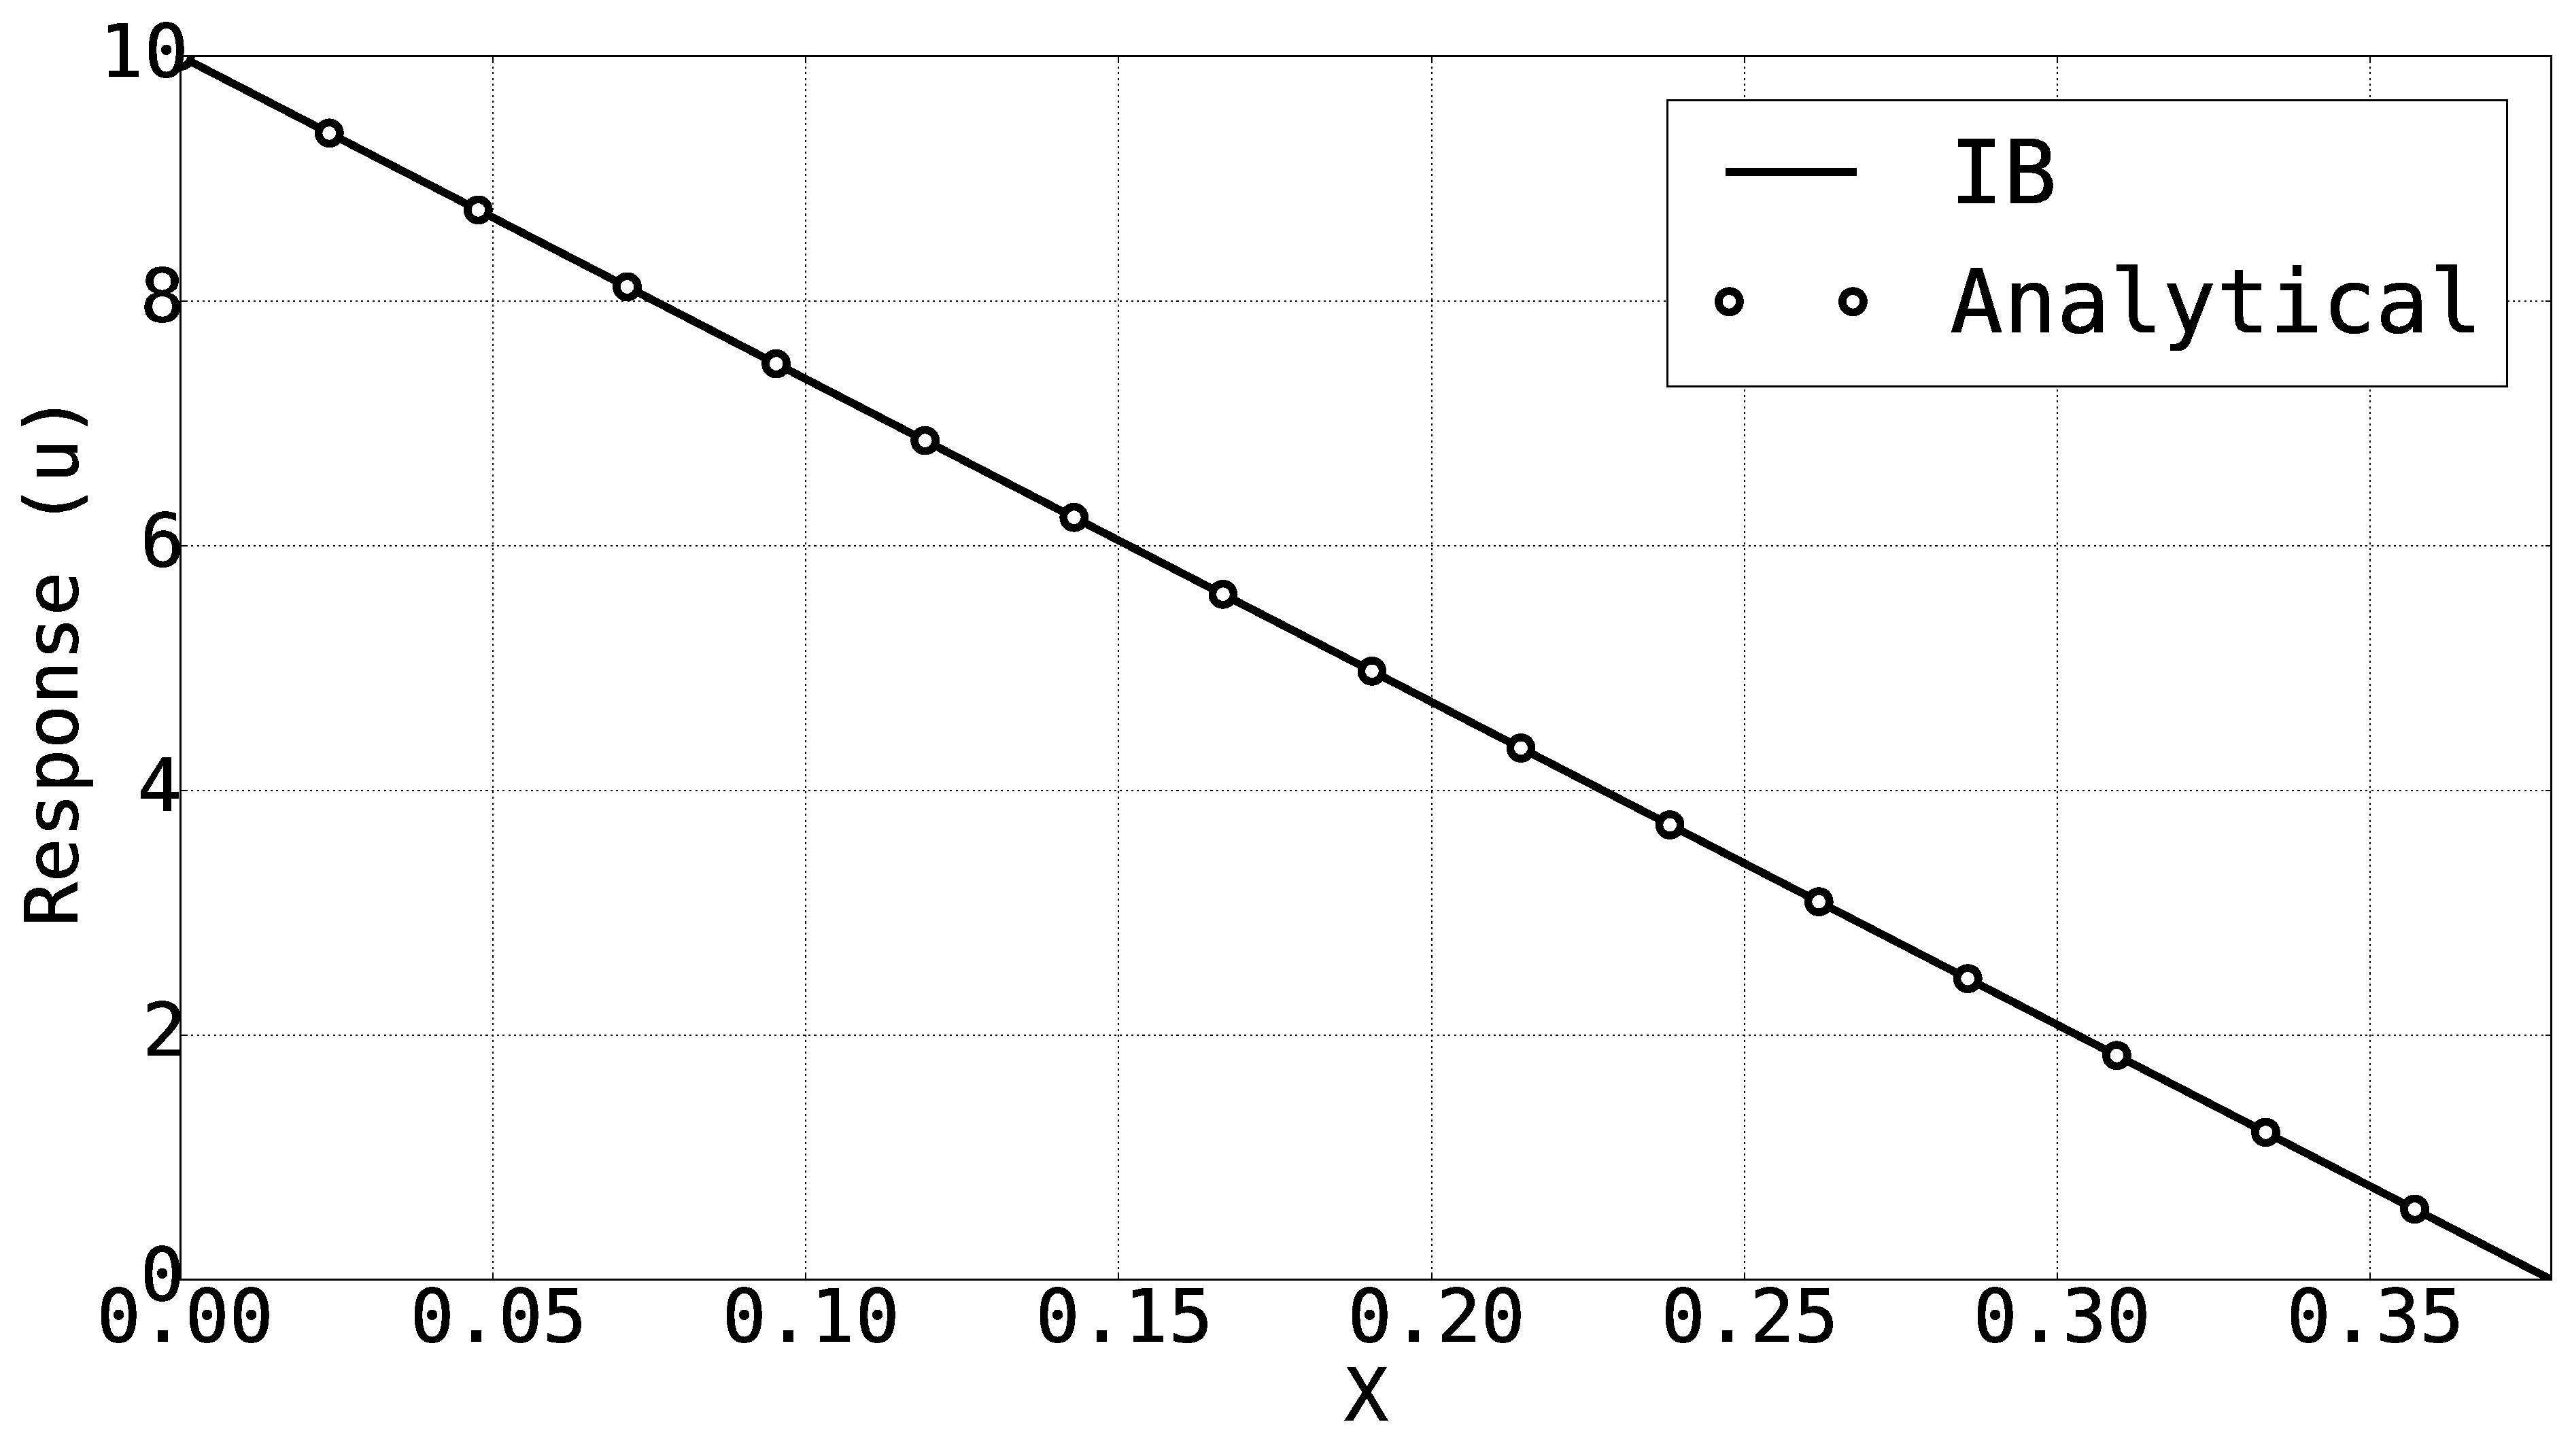
\includegraphics[width=7.0cm]{Chapter_3/figure/ghostCell_wallLocation_379.eps}
	}
	\\
	\subfigure[N = 81]
	{
	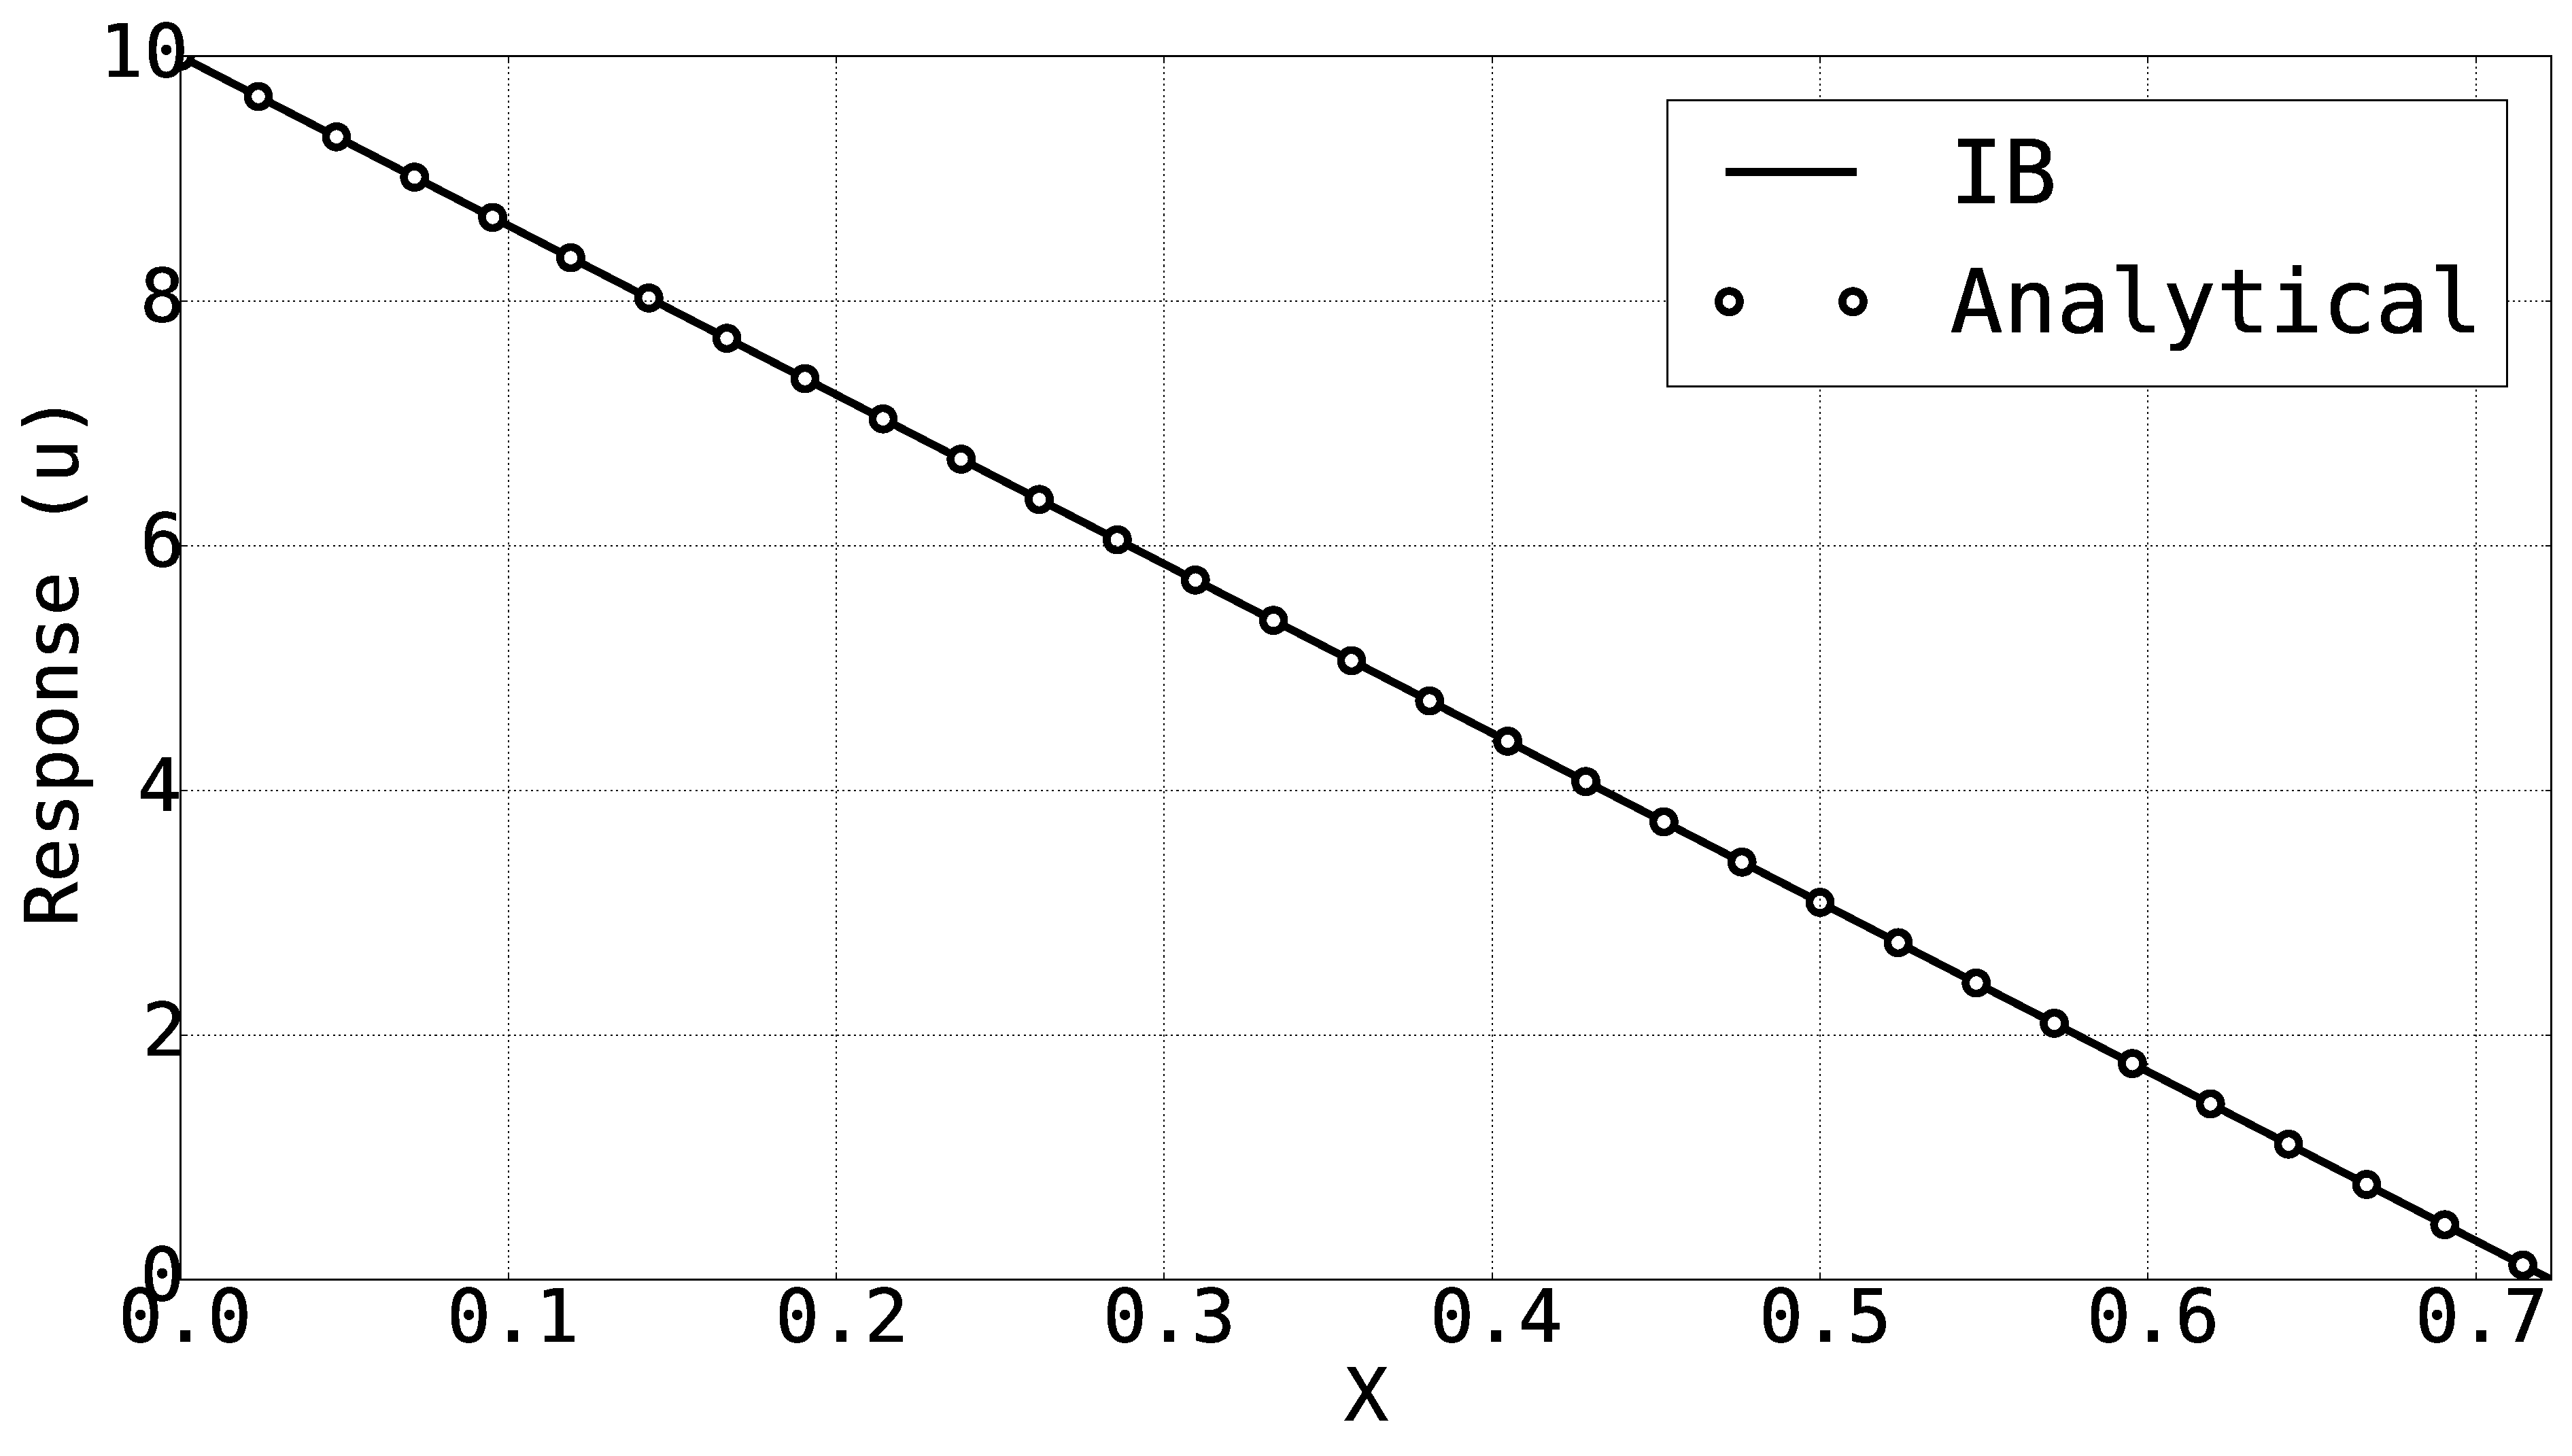
\includegraphics[width=7.0cm]{Chapter_3/figure/ghostCell_wallLocation_723.eps}
	}
	\quad
	\subfigure[N = 161]
	{
	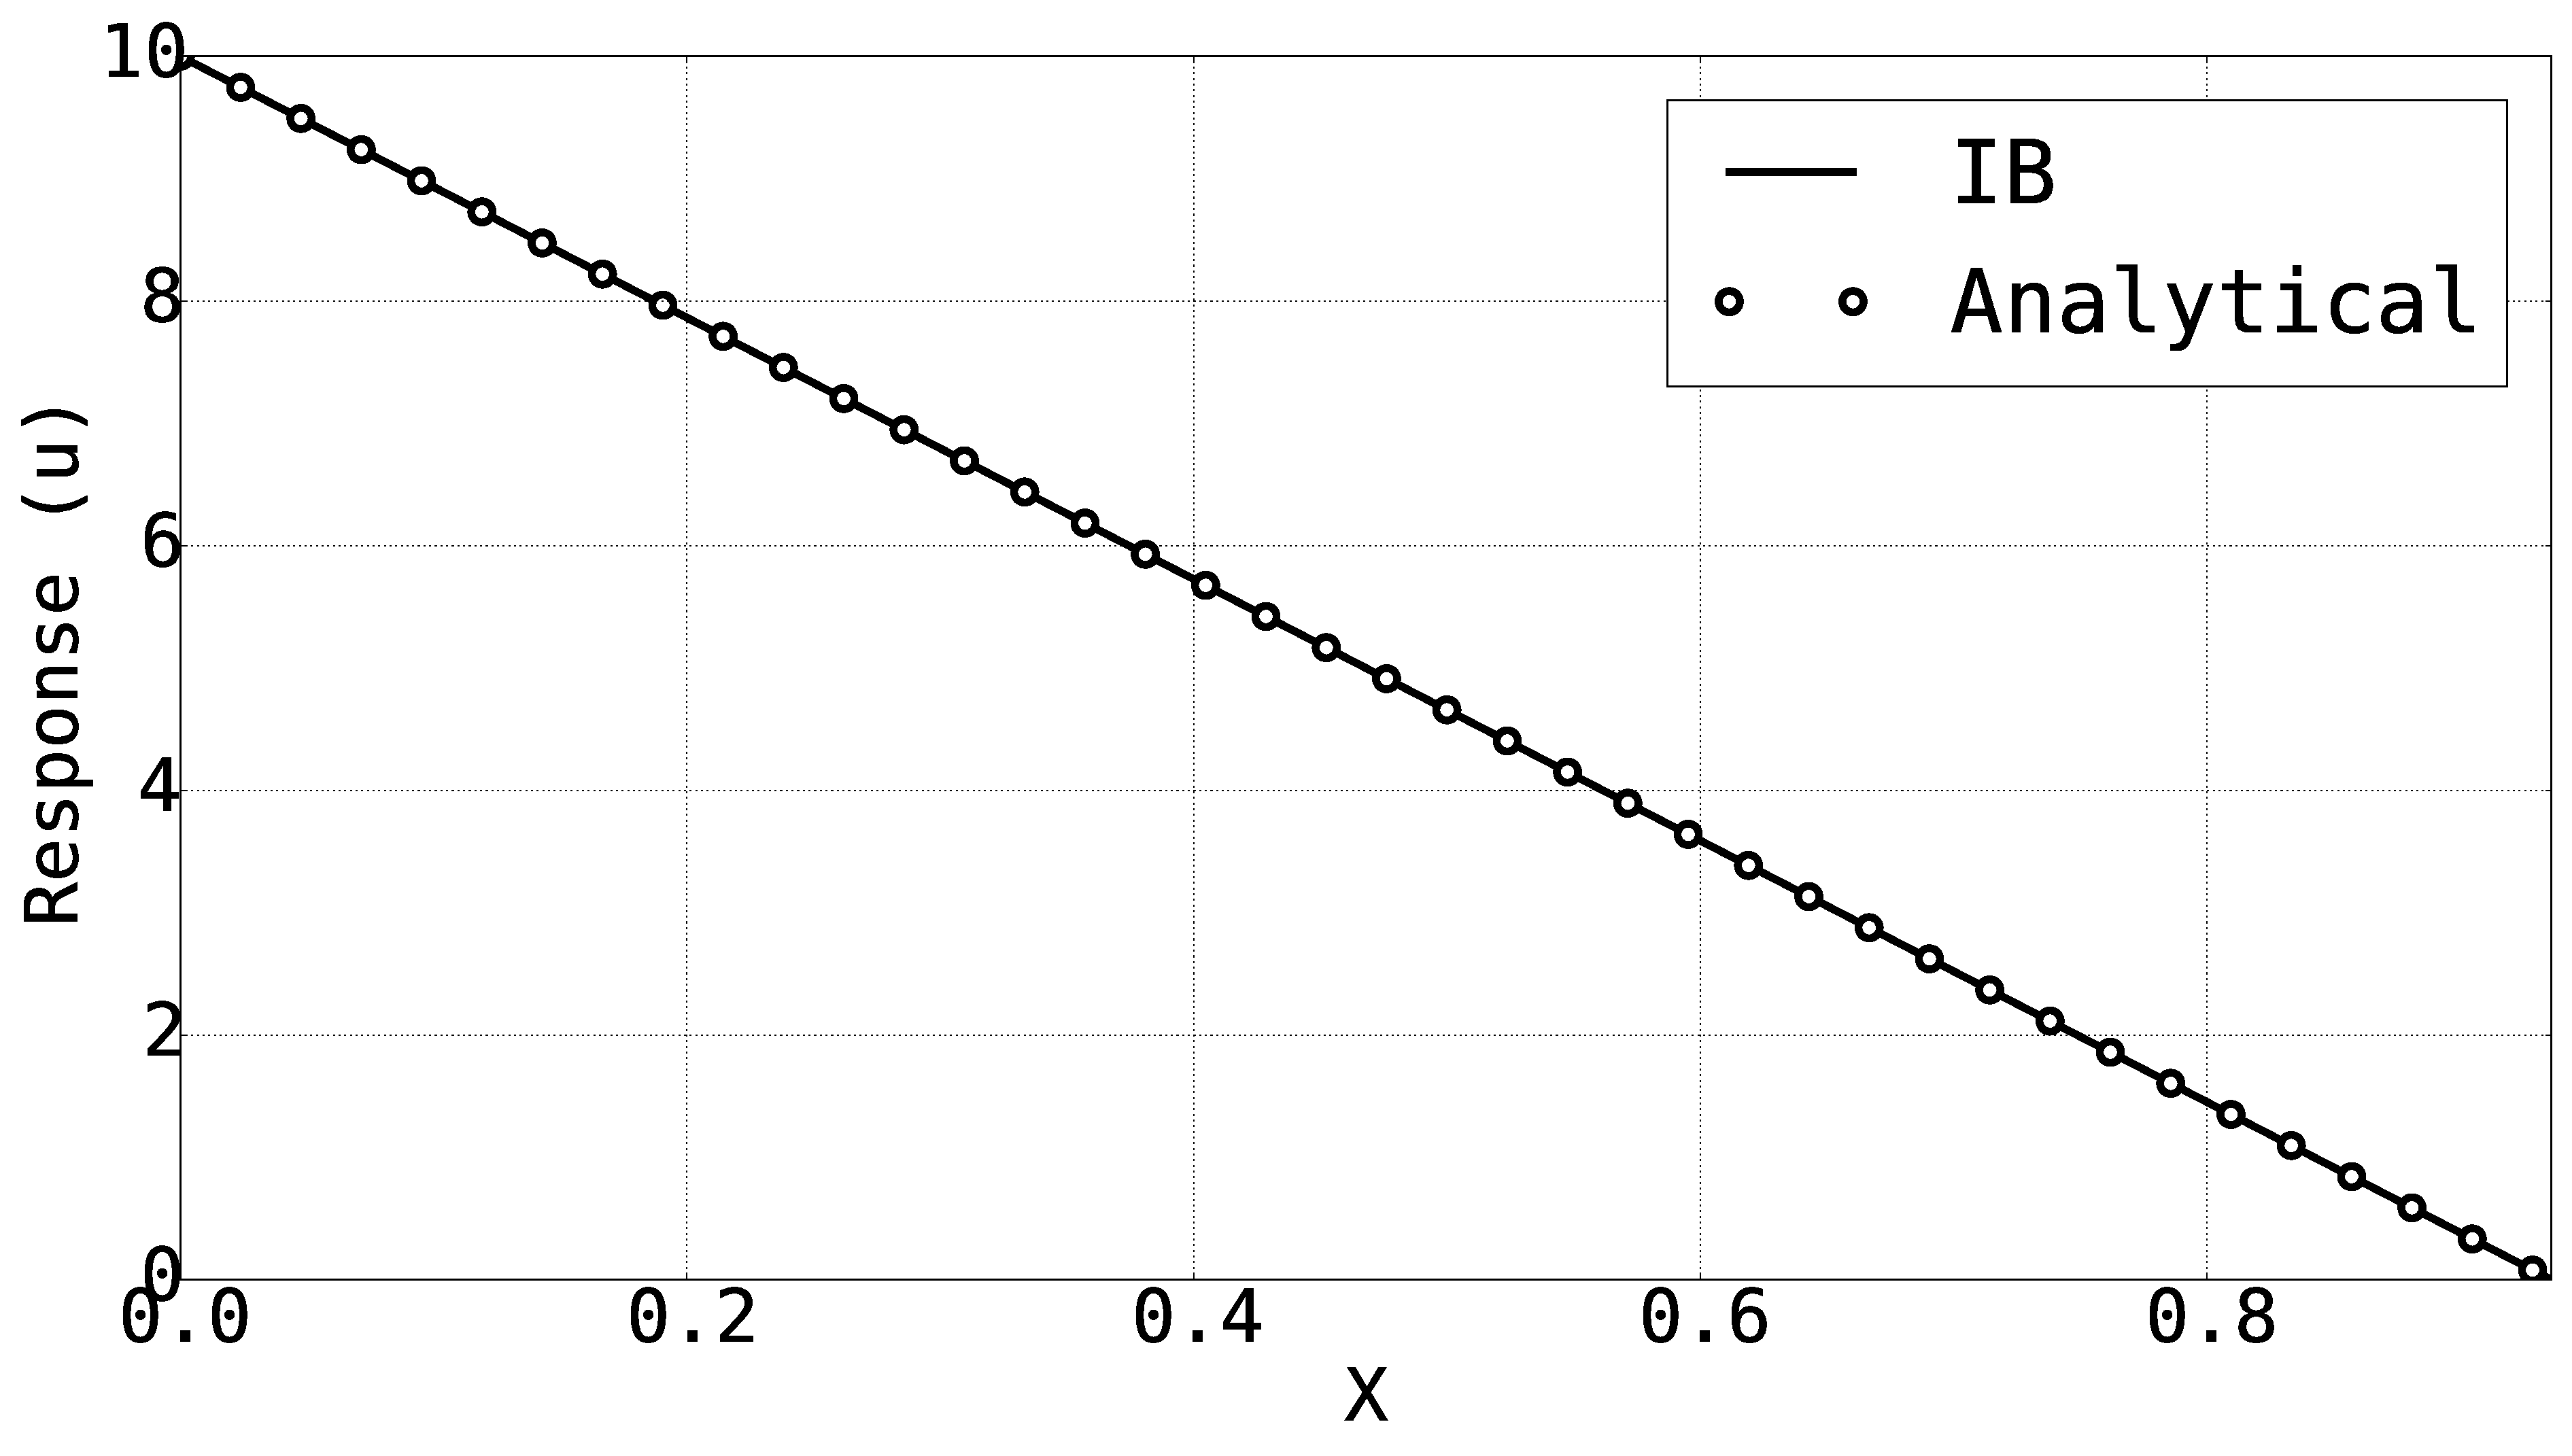
\includegraphics[width=7.0cm]{Chapter_3/figure/ghostCell_wallLocation_936.eps}
	}
	\caption{Comparison between IB and analytical results for different wall location.}
	\label{fig:C3_ghostCell_wallLocation}
\end{figure}

\begin{table}[H]
\centering
\begin{tabular}{c | c}
	 Wall location & RMSE value \\ \hline \hline
	 0.124 & 5.49E-17 \\ \hline
	 0.379 & 3.16E-15 \\ \hline
	 0.723 & 2.72E-14 \\ \hline
	 0.936 & 4.99E-14
\end{tabular}
\caption{RMSE value for different wall location.}
\label{table:C3_ghostCell_wallLocation_RMSE}
\end{table}

For the final investigation, we looked at the effect of wall velocity of the solution accuracy. For this case, the number of nodes is fixed as $41$ and the stationary wall is located at $x_{wall} = 0.479$. The moving wall velocity is selected as $100$, $1000$, $10000$, and $100000$. As shown in Figure \ref{fig:C3_ghostCell_wallVelocity} and Table \ref{table:C3_ghostCell_wallVelocity_RMSE}, the wall velocity does not affect the accuracy of the solution.

\begin{figure}[H]
	\centering
	\subfigure[N = 11]
	{
	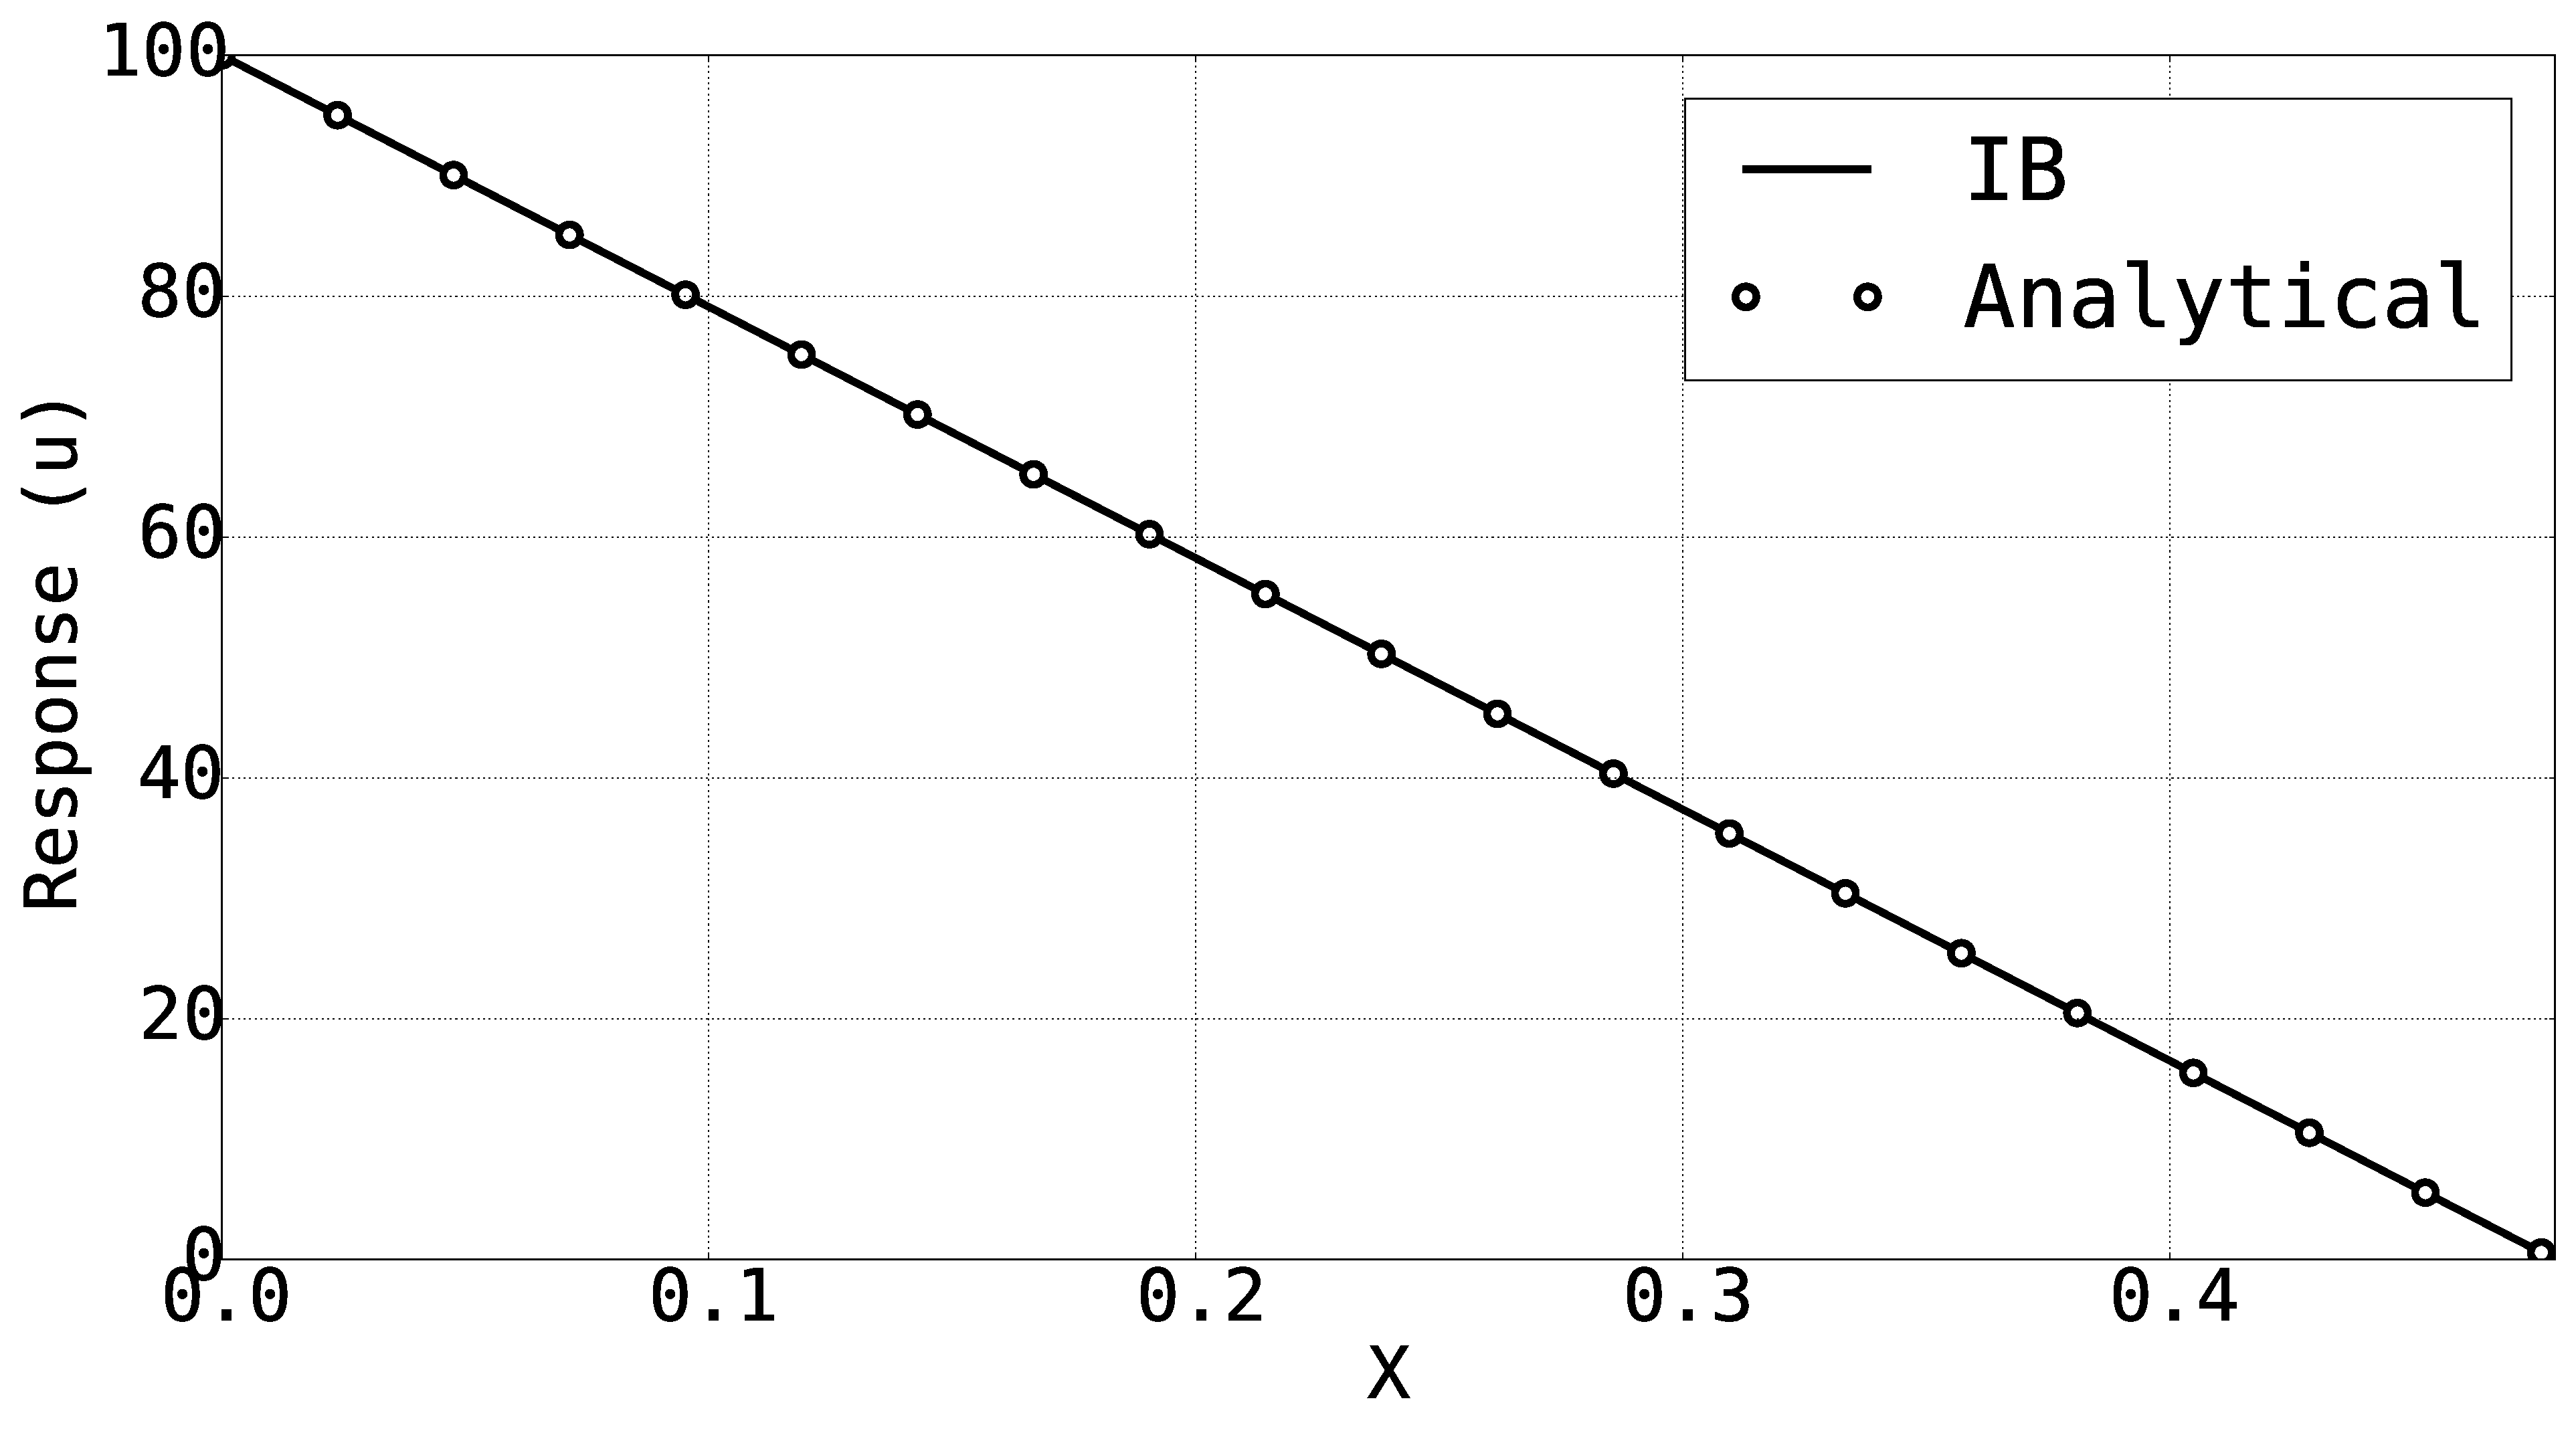
\includegraphics[width=7.0cm]{Chapter_3/figure/ghostCell_wallVelocity_100.eps}
	}
	\quad
	\subfigure[N = 41]
	{
	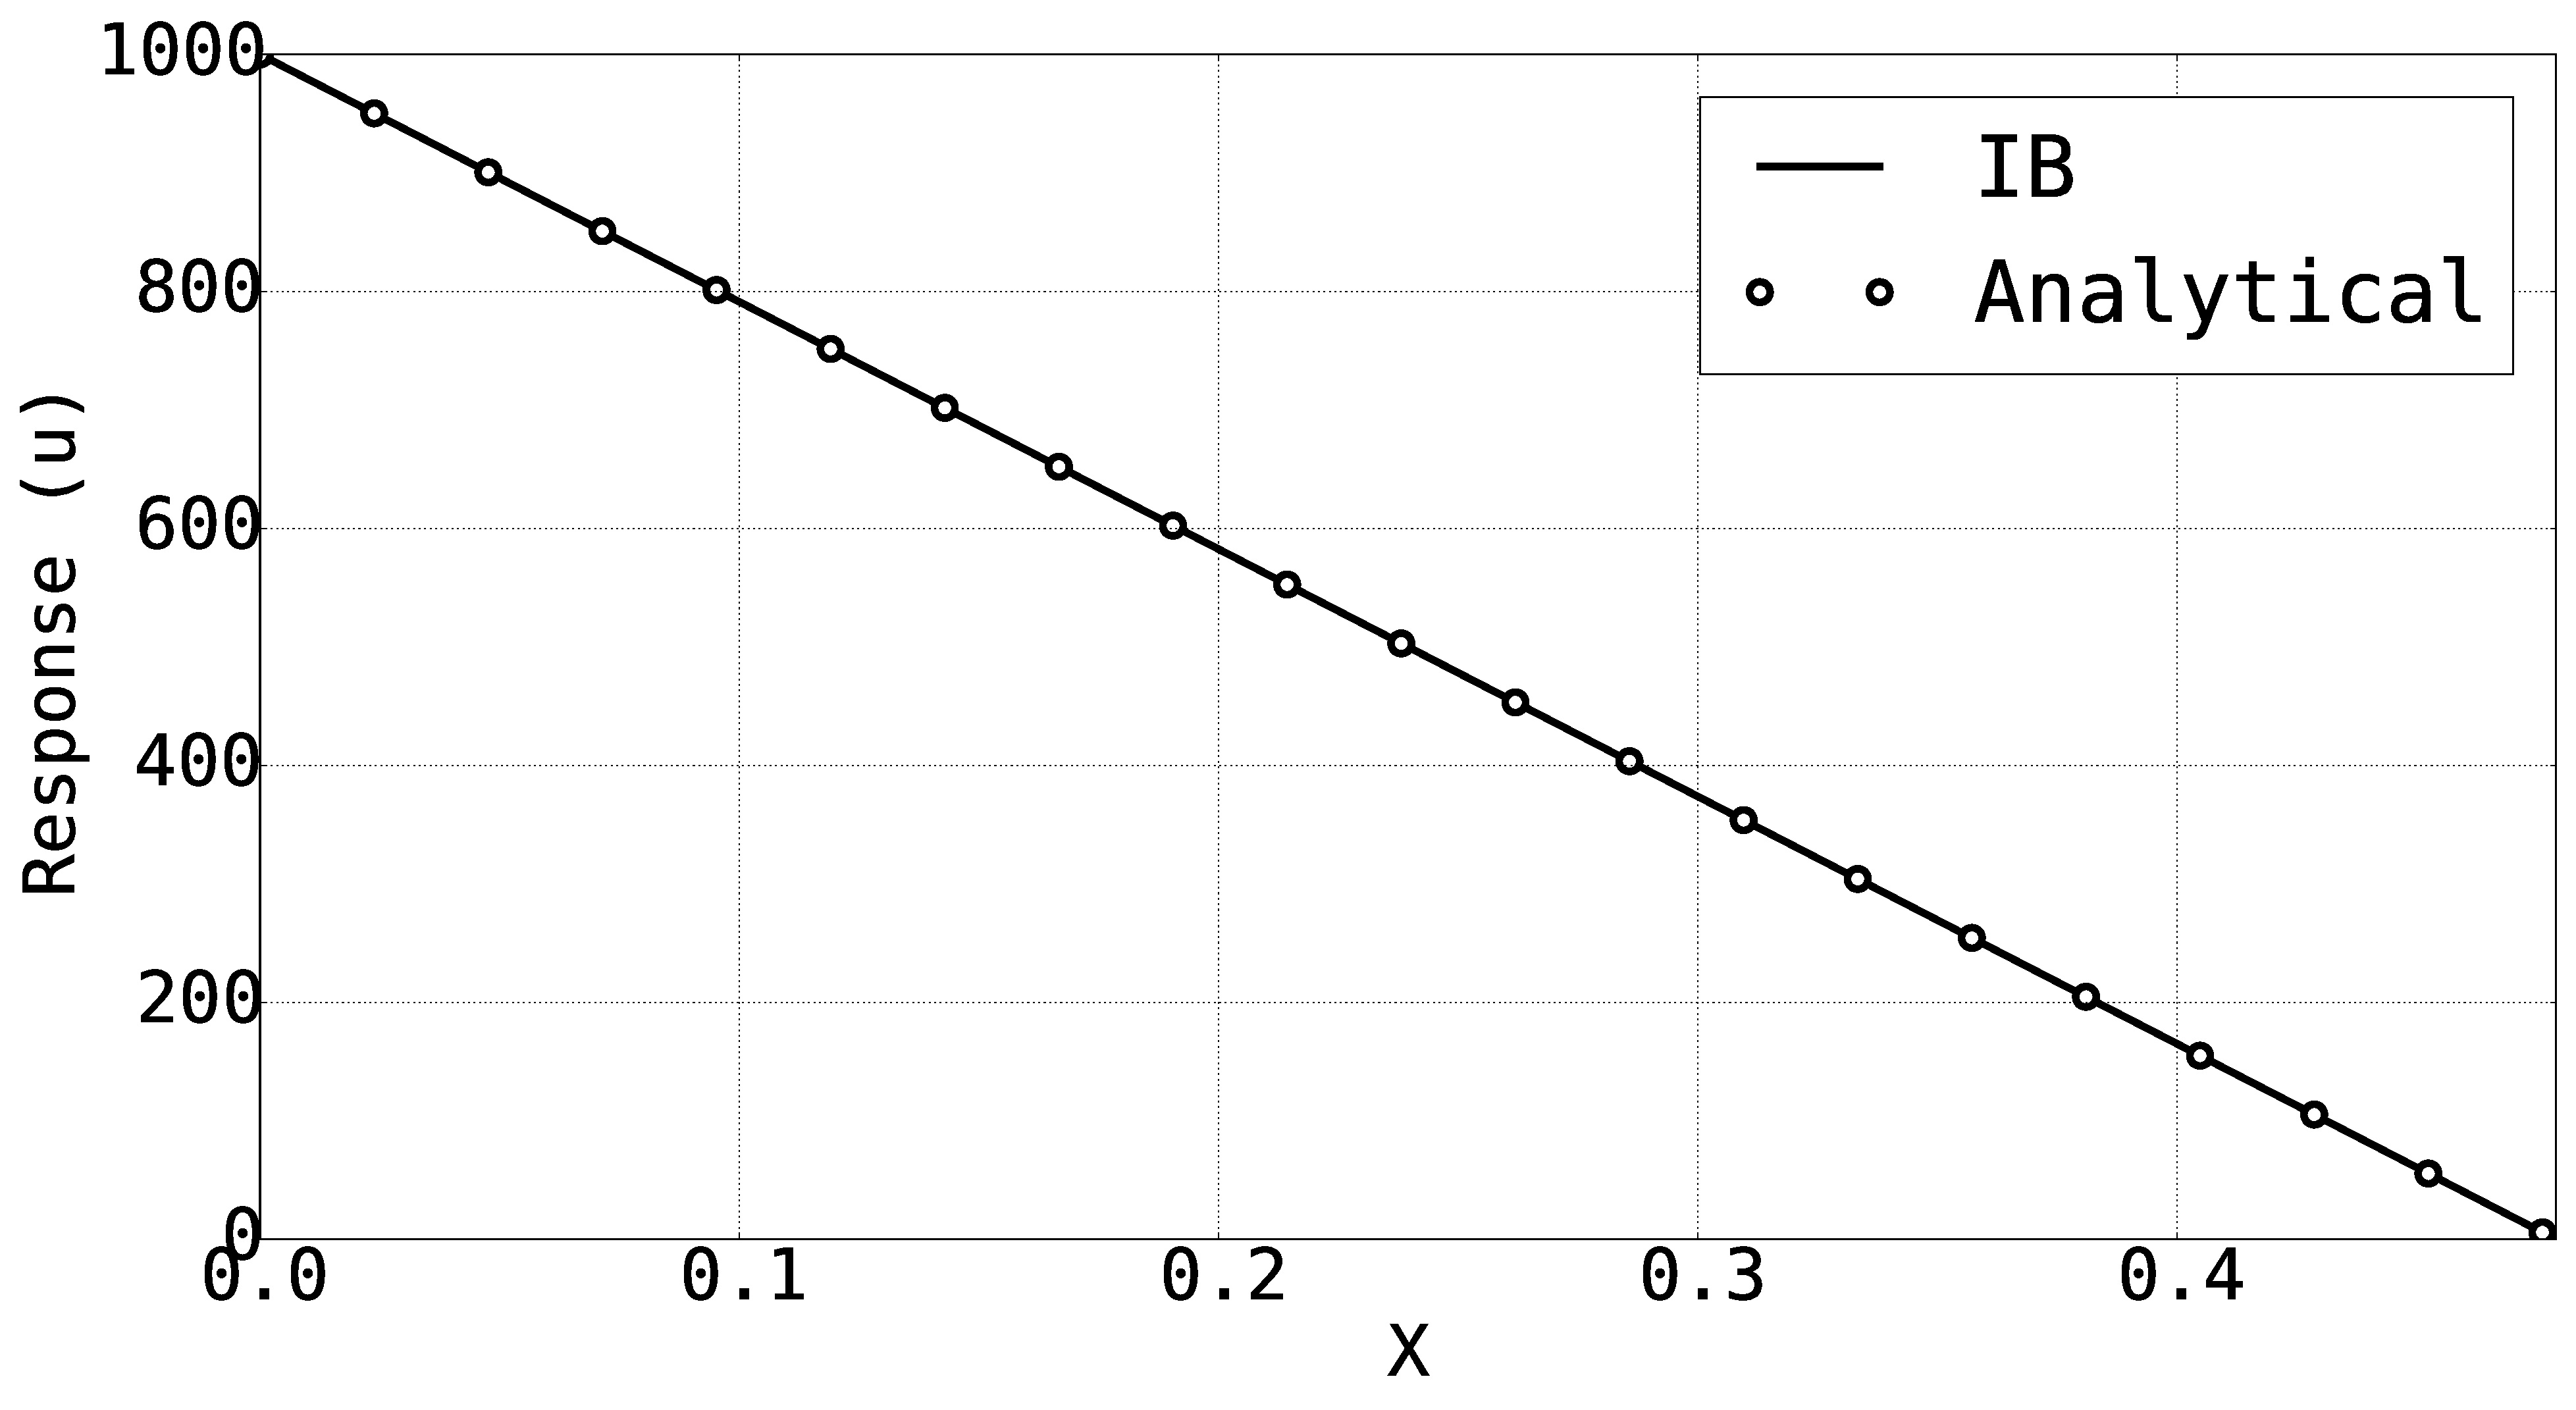
\includegraphics[width=7.0cm]{Chapter_3/figure/ghostCell_wallVelocity_1000.eps}
	}
	\\
	\subfigure[N = 81]
	{
	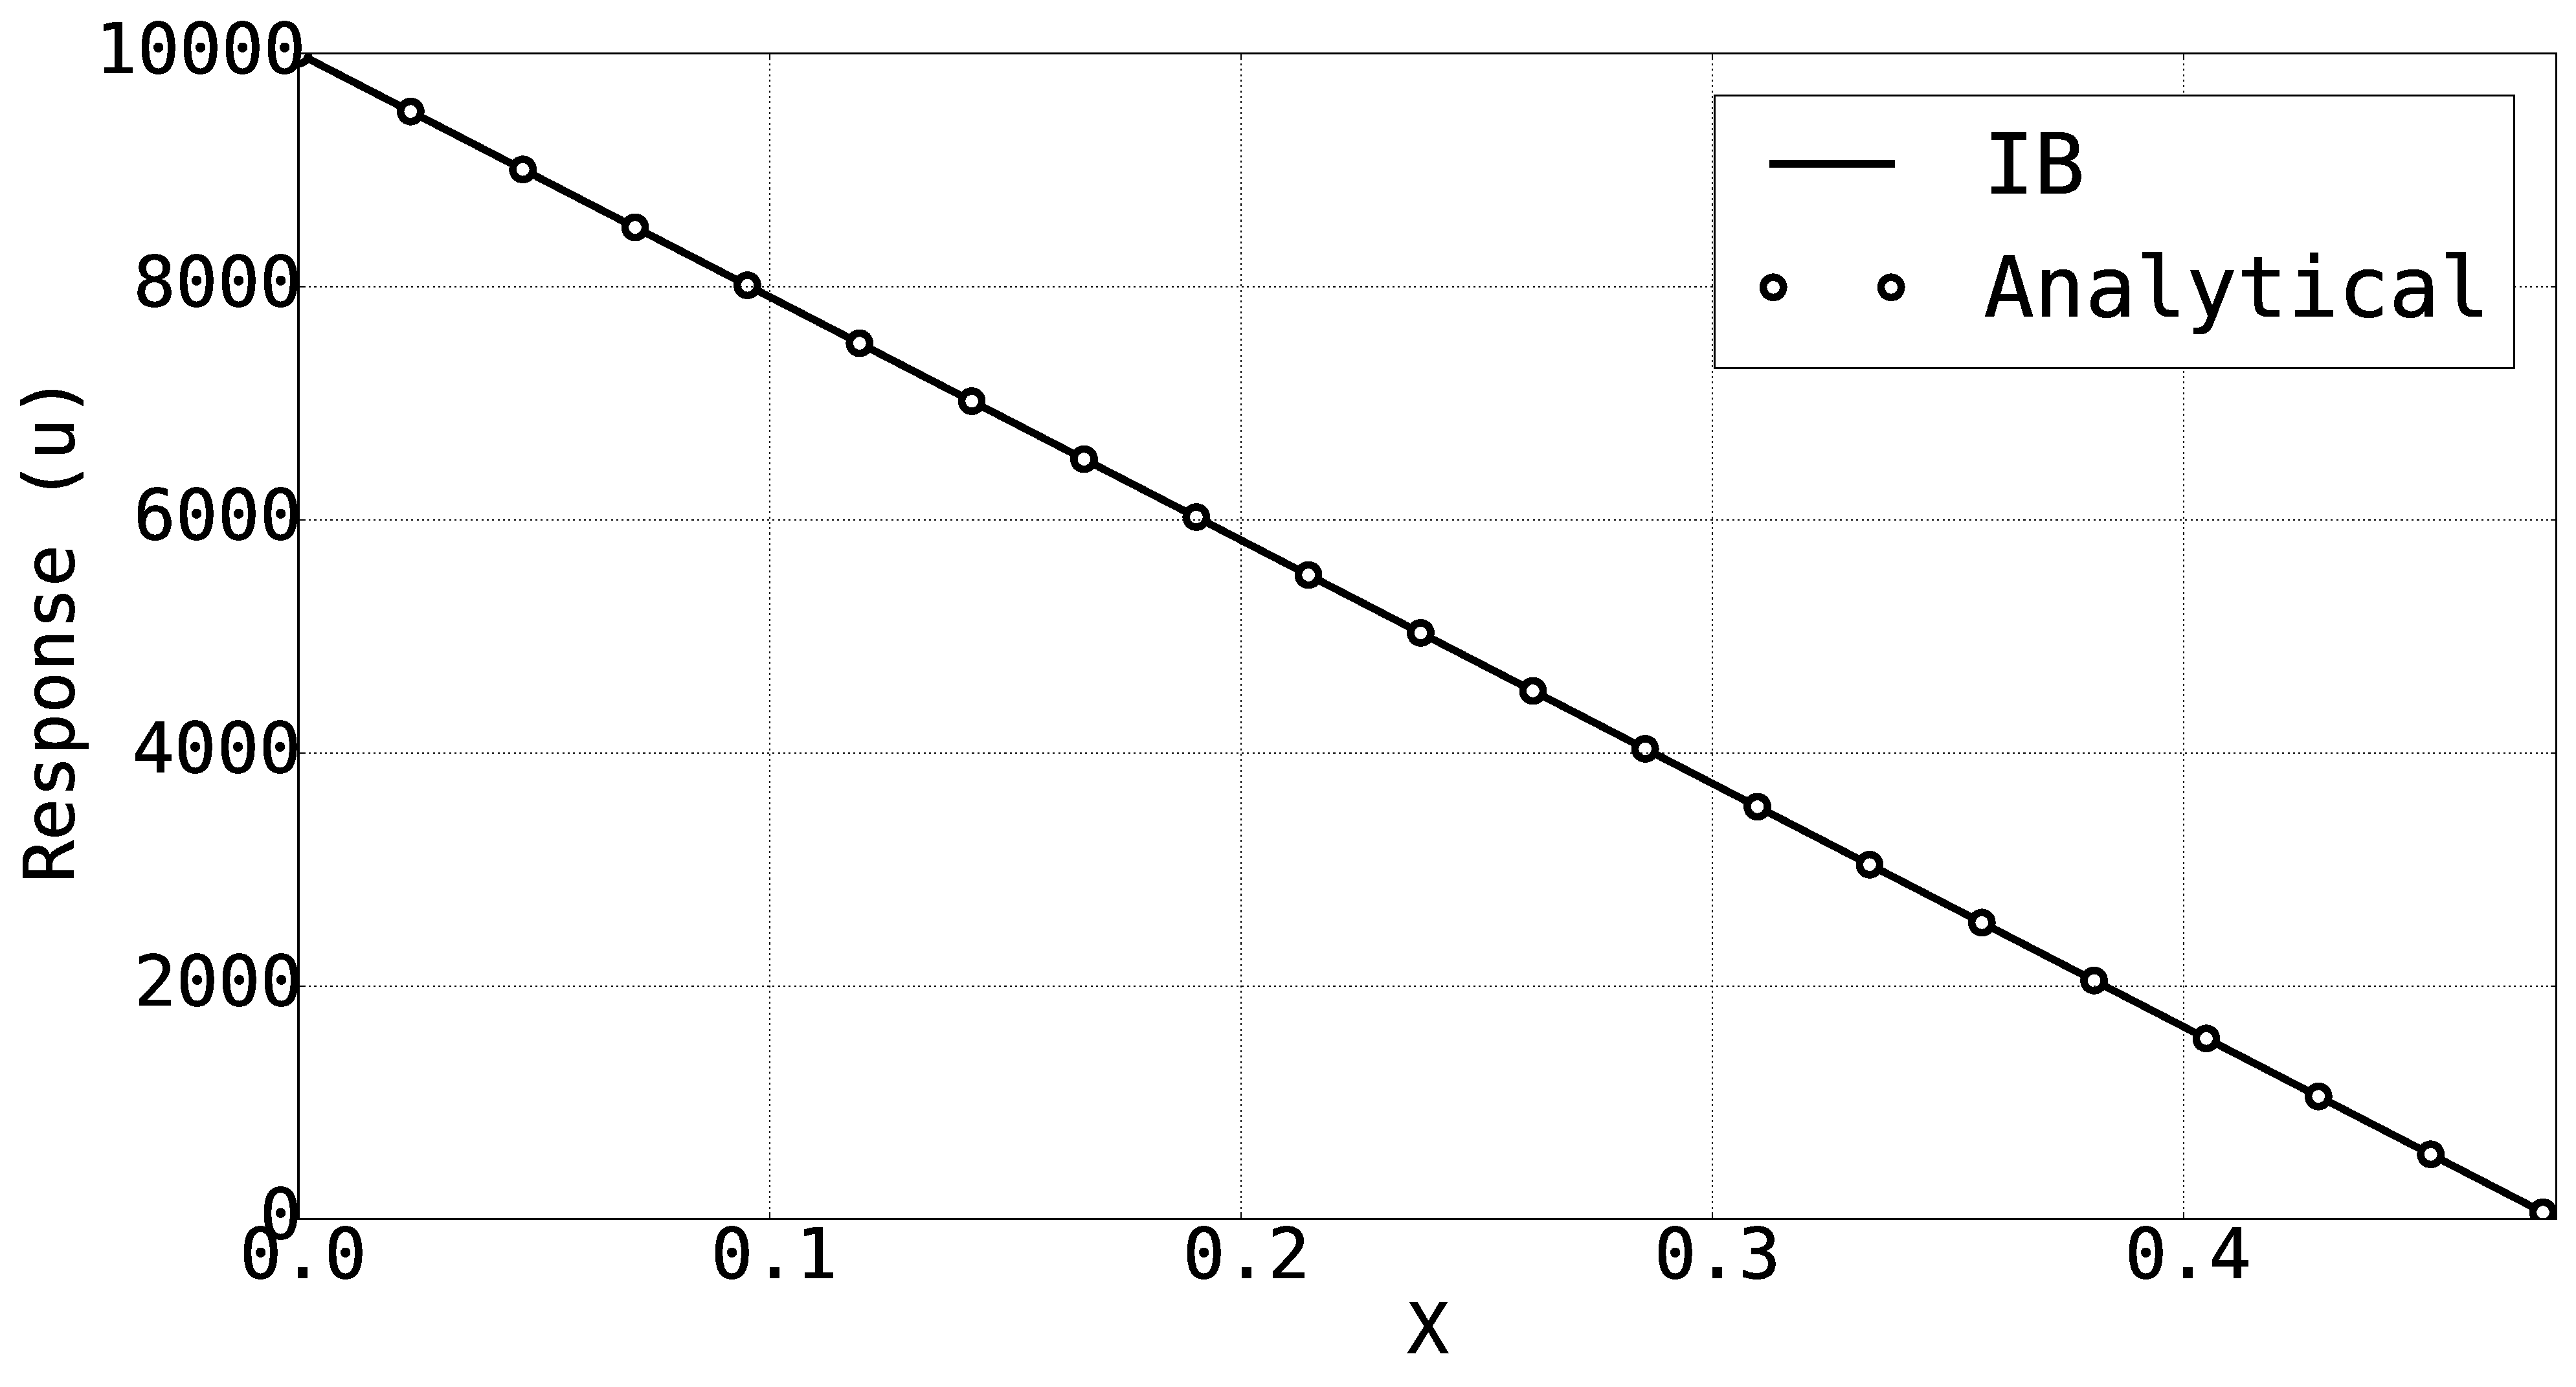
\includegraphics[width=7.0cm]{Chapter_3/figure/ghostCell_wallVelocity_10000.eps}
	}
	\quad
	\subfigure[N = 161]
	{
	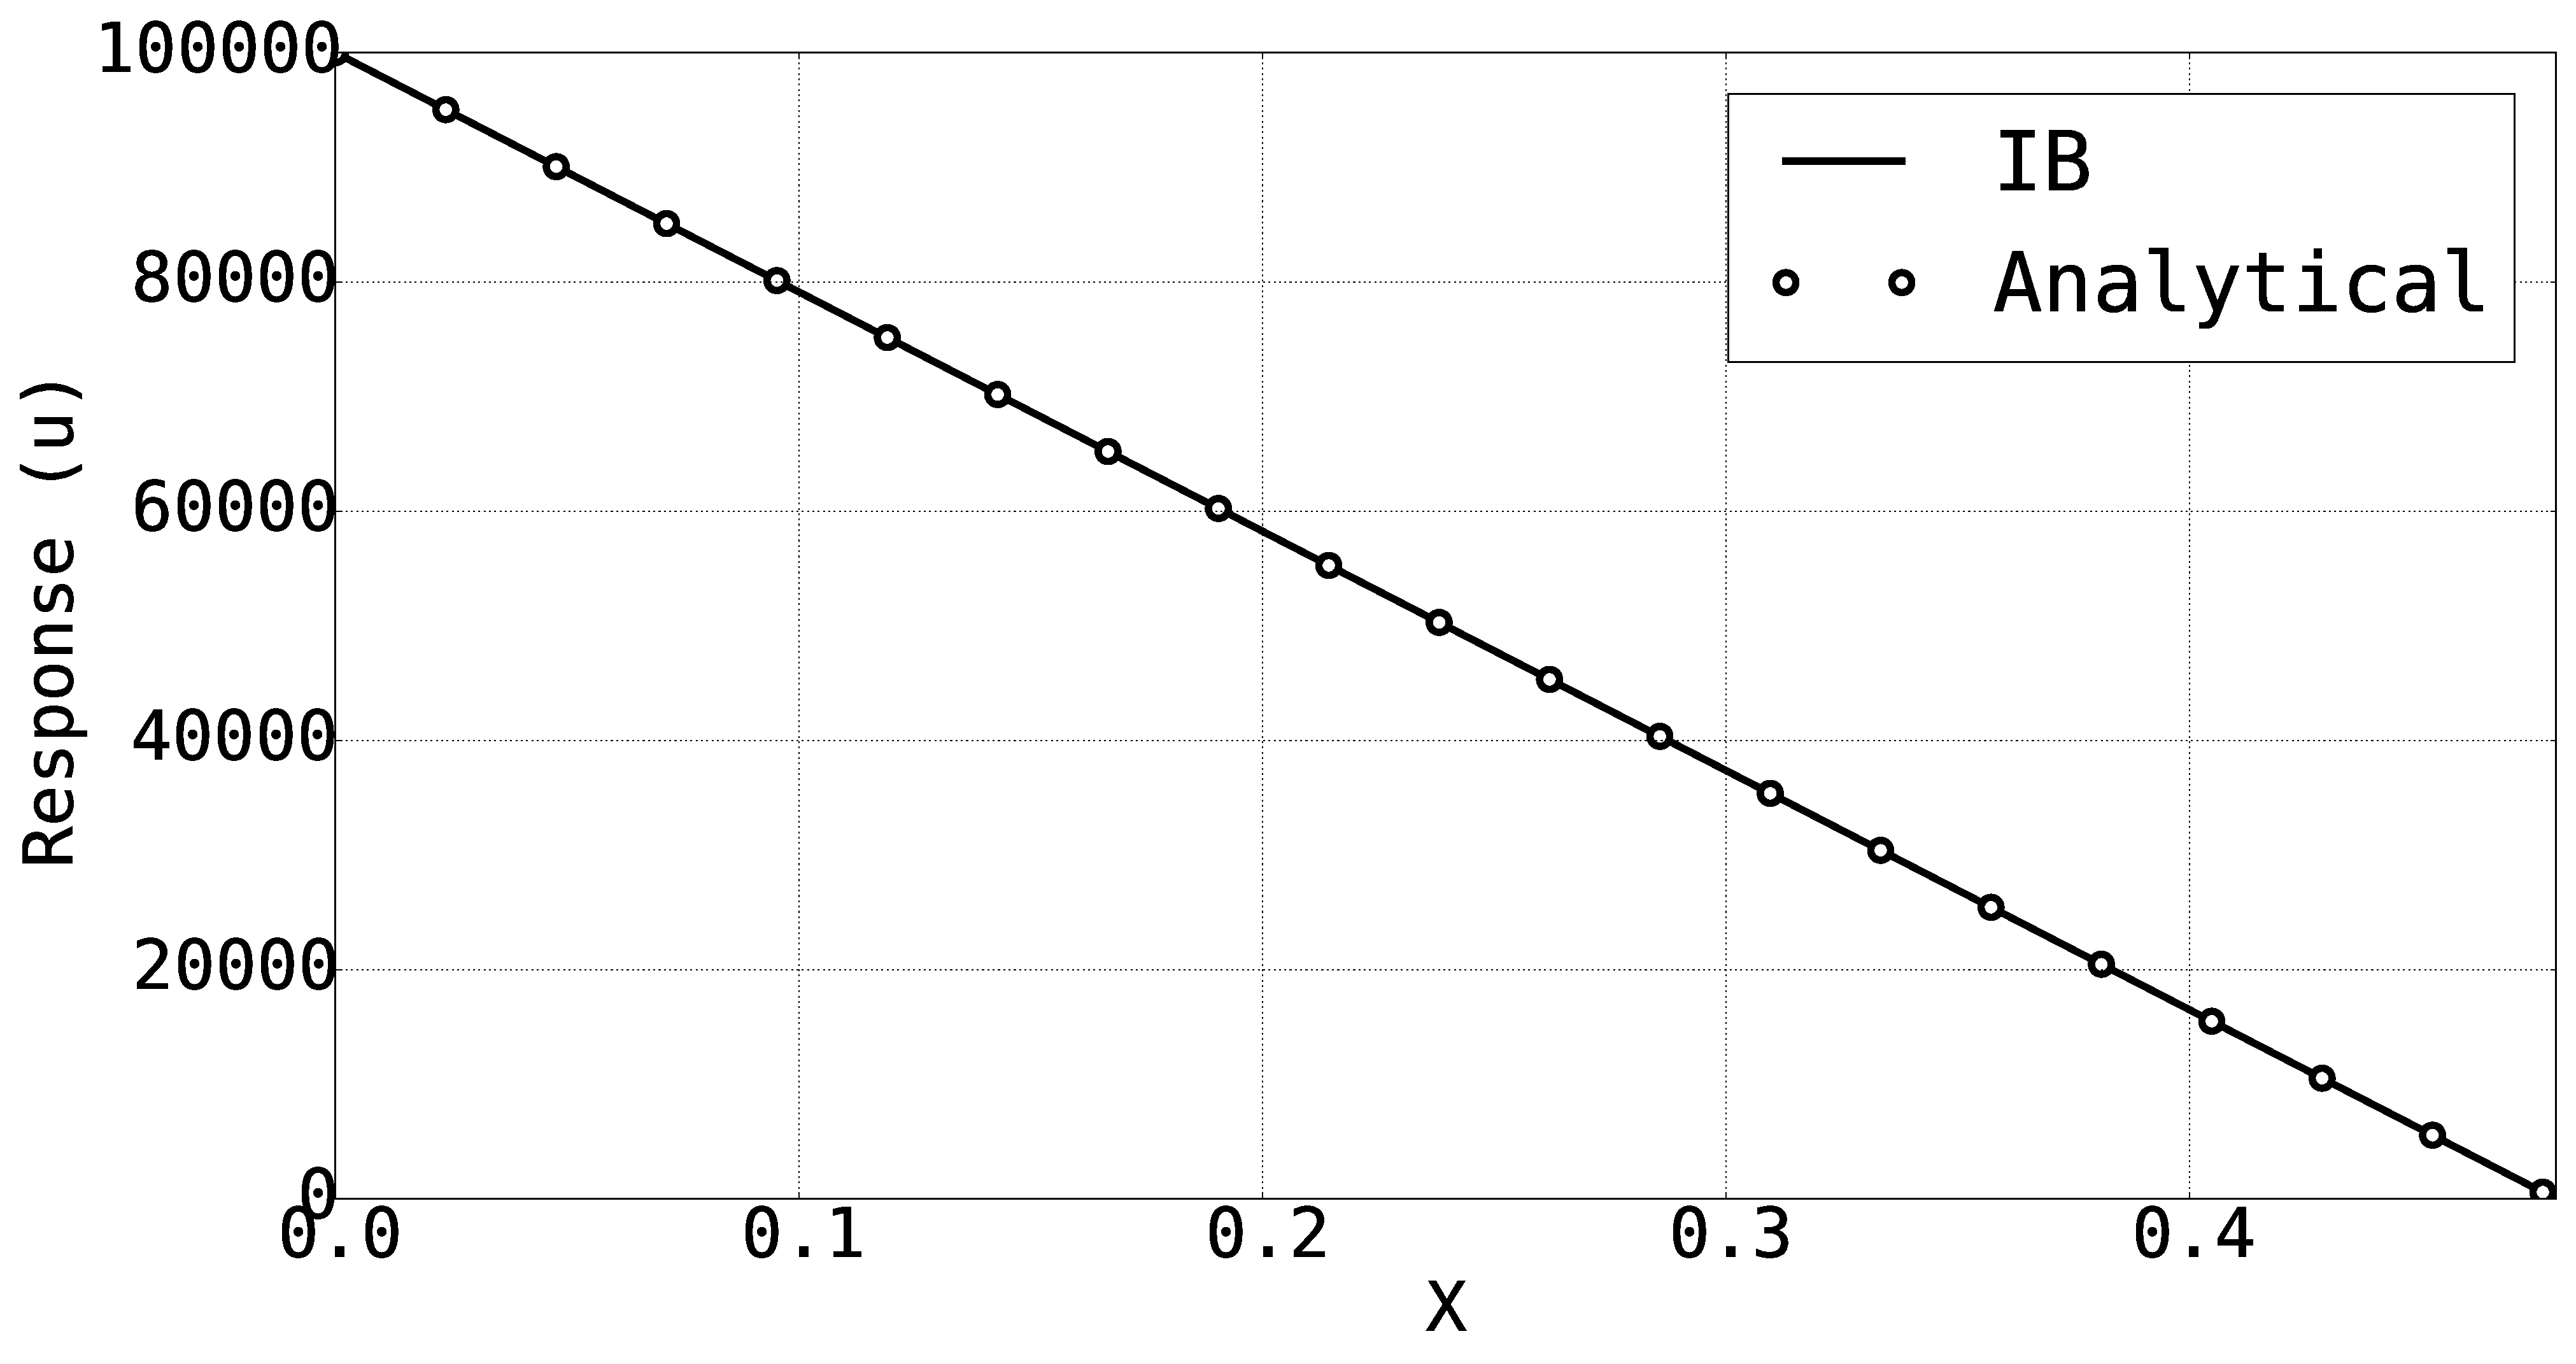
\includegraphics[width=7.0cm]{Chapter_3/figure/ghostCell_wallVelocity_100000.eps}
	}
	\caption{Comparison between IB and analytical results for different wall velocities.}
	\label{fig:C3_ghostCell_wallVelocity}
\end{figure}

\begin{table}[H]
\centering
\begin{tabular}{c | c}
	 Wall velocity & RMSE value \\ \hline \hline
	 100 & $8.89 \times 10^{-15}$ \\ \hline
	 1000 & $8.36 \times 10^{-15}$ \\ \hline
	 10000 & $8.31 \times 10^{-15}$ \\ \hline
	 100000 & $8.62 \times 10^{-15}$ \\ \hline
\end{tabular}
\caption{RMSE value for different wall velocities.}
\label{table:C3_ghostCell_wallVelocity_RMSE}
\end{table}